%=====================================================================================================
% Document formatting and packages
%=====================================================================================================

\documentclass[10pt]{article}
\setlength\topmargin{0in}
\setlength\headheight{0in}
\setlength\headsep{0in}
\setlength\textheight{9in}
\setlength\textwidth{6.5in}
\setlength\oddsidemargin{0in}
\setlength\evensidemargin{0in}
\setlength\parindent{0.25in}
\setlength\parskip{0in}
\usepackage{amsmath}
\usepackage{bm}													% required for bold equations
\usepackage{graphicx}										% required for images
\usepackage{epstopdf}										% require for .eps graphics
\usepackage{float}											% allows [H] to be used for floats (forces float to appear at location in code)
\usepackage[usenames,dvipsnames]{color}
\usepackage[pdftex]{hyperref} 					% creates bookmarks and all cross-references and citations are hyperlinked in pdf
\hypersetup{bookmarksnumbered, 					% put section numbers in bookmarks
						bookmarksopen=false,
						colorlinks = true,
						linkcolor=MidnightBlue,
						citecolor=MidnightBlue,
						urlcolor=MidnightBlue}			% bookmarks expanded when pdf opened

%=====================================================================================================
% My Macros
%=====================================================================================================

%\DeclareFixedFootnote{\gyrofootnote}{x-IMUs of generations prior to version 1.3 use the \href{http://www.x-io.co.uk/res/doc/itg3200.pdf}{ITG-3200} gyroscope.}

%\def x-IMU GUI {\href{http://www.x-io.co.uk/node/9\#ximu_gui}{x-IMU GUI}}
%\def x-IMU API {\href{http://www.x-io.co.uk/node/9\#ximu_api}{x-IMU API}}
\def \MATLAB {\href{http://www.x-io.co.uk/node/10\#ximu_matlab_library}{MATLAB}}
\def \accelMagName {\href{http://www.x-io.co.uk/res/doc/lsm303dlh.pdf}{LSM303DLH}}
\def \gyroName {\href{http://www.x-io.co.uk/res/doc/imu3000.pdf}{
IMU-3000}}

\def \contactUs {\href{http://www.x-io.co.uk/contact}{contact us}}
\def \sectionComingSoon {This section is currently unavailable but can be updated \href{http://www.x-io.co.uk/contact}{on request}.}

%=====================================================================================================
% Title, Name, Date
%=====================================================================================================

\title{\Huge x-IMU User Manual 5.1 \normalsize}
\author{x-io Technologies}

\begin{document}

%---------------------------------------------------------------------------------------------------
\begin{titlepage}

	\maketitle
	\vspace{20 mm}
	\begin{figure}[H]
		\centering
			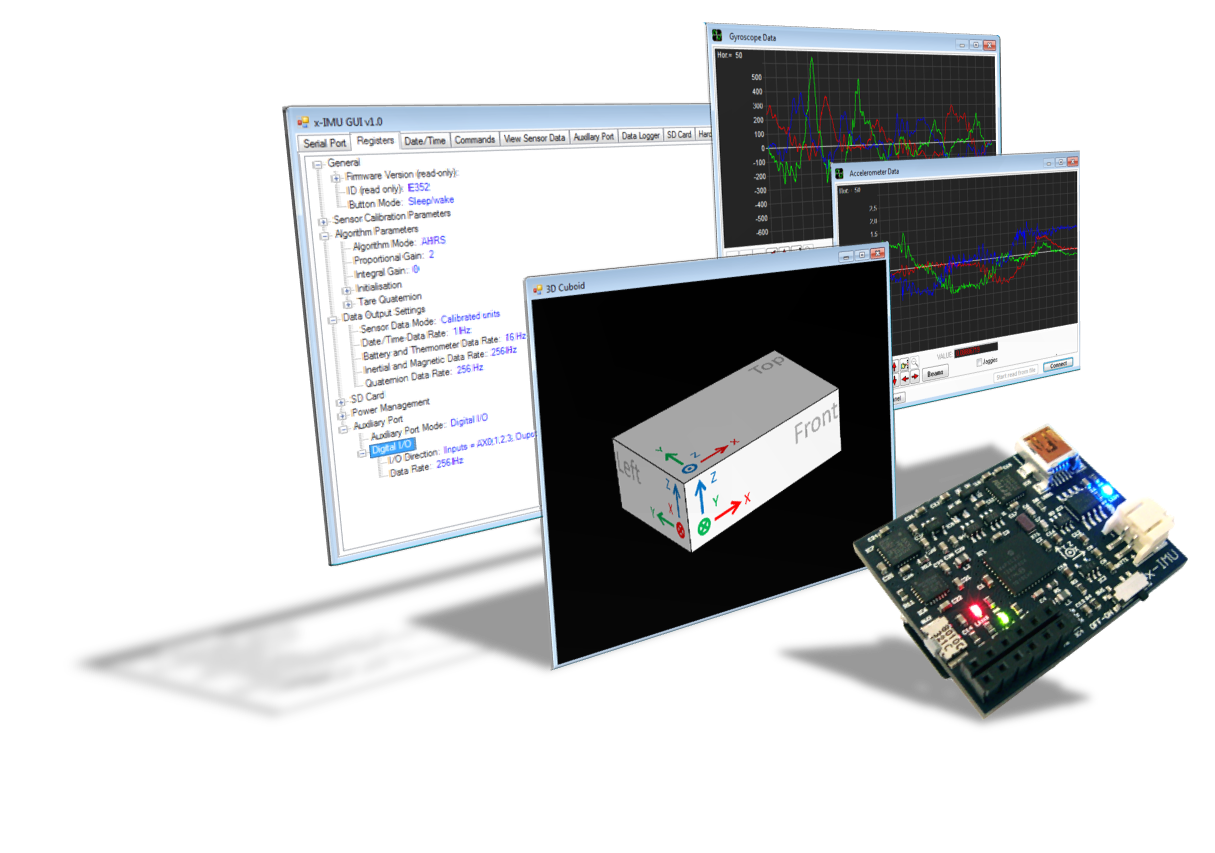
\includegraphics[width=0.8\textwidth]{graphics/ximu_software_large.png}
	\end{figure}

\end{titlepage}

%%=====================================================================================================
%% Version history
%%=====================================================================================================
%%\section{Version history}
%%\label{sec:VersionHistory}
%
%
% TO DO:!!!!!!!!!!!!!!!!!!!!!!!!!!!!!!!!!!!!!!!!
% - AHRS re-init when mode register written to
% - gyro cal model uses AHRS biases
%
%
%
%
%\begin{table}[H]
%	\centering
%		\begin{tabular*}{1.0\textwidth}{l l p{0.75\textwidth}}
%			\hline
%			Version	&	Date				& Notes\\
%			\hline\\
%			2.1			& 17/05/2011	&	- Minor corrections spelling/wording/layout/appearance througout.\\
%							&							& - IMU/AHRS algorithm section has been updated.\\
%							&							& - TODO: link to API docuemtnation etc.\\
%			2.0			& 17/05/2011	&	- Minor corrections spelling/wording/layout/appearance througout.\\
%							&							& - Documented changes introduced by firmware 5.0, API 8.0 and GUI 7.0.  See individual release notes for details.\\
%							&							& Compatible versions: firmware 5.x, GUI 7.x, API 8.x.\\
%			1.0			& 10/05/2011	&	- Initial release.\\
%							&							& Compatible versions: firmware 4.x, GUI 6.x, API 7.x.\\
%			\hline
%		\end{tabular*}
%		\caption{Document version history}
%\end{table}
%
%%If you have any suggestions for how this document could be improved, please \href{ http://www.x-io.co.uk/contact}{contact us} and let us know.

%=====================================================================================================
\section*{Disclaimer}
\label{sec:Disclaimer}

\textit{The x-IMU and associated software are provided in an `as in' condition.  No warranties, whether express, implied or statutory, including but not limited to implied warranties of merchantability and fitness for a particular purpose apply.  x-io Technologies shall not in any circumstances, be liable for special, incidental or consequential damages, for any reason whatsoever.}

\newpage
%=====================================================================================================
\tableofcontents

\newpage
%=====================================================================================================
\section{x-IMU overview}
\label{sec:xIMUOverview}

The x-IMU was designed to be the most versatile Inertial Measurement Unit (IMU) and Attitude Heading Reference System (AHRS) product available. Its host of on-board sensors, algorithms and configurable 8-channel auxiliary port make the x-IMU both a powerful sensor and controller. Communication is enabled via USB or Bluetooth for wireless applications. The on-board SD card, battery charger (via USB), real-time clock/calendar and motion trigger wake up also make the x-IMU an ideal stand-alone data logger.

The open source x-IMU GUI{} allow users configure all internal x-IMU settings, view sensor data in real-time and export data to software such as \MATLAB{} and Microsoft Excel. Custom user software may be developed using the x-IMU API{}.

\subsection{x-IMU Features}
\label{sec:xIMUFeatures}

\paragraph{On-board sensors}
\begin{itemize}
	\item Triple axis 16-bit gyroscope - Selectable range up to $\pm2000^\circ$/s
	\item Triple axis 12-bit accelerometer - Selectable range up to $\pm8$ g
	\item Triple axis 12-bit magnetometer - Selectable range up to $\pm8.1$ G
	\item 16-bit thermometer
	\item 12-bit battery voltage level
	\item Factory calibrated
	\item Temperature compensated (gyroscope only)
	\item Selectable data rates up to 512 Hz
\end{itemize}

\paragraph{On-board algorithms}
\begin{itemize}
    \item IMU and AHRS algorithms provide real-time measurement of orientation relative to the Earth
    \item Internal states updated at 512 Hz
    \item Algorithm `initialise' and 'tare' commands can be sent in real-time
    \item Complete sensor calibration algorithms for user maintenance
\end{itemize}

\paragraph{Connectivity}
\begin{itemize}
    \item USB
    \item Bluetooth - Class 1, 100m range, SPP
    \item Micro SD card - Supports FAT16/32 and SDHC
    \item UART (see \hyperref[sec:UART]{auxiliary port mode})
\end{itemize}

\paragraph{Power options}
\begin{itemize}
    \item USB
    \item LiPo battery - On-board charging via USB
    \item External source from 3.6 V to 6.3 V
    \item Low power consumption - 50 mA to 150 mA dependent on settings and usage, 130 �A sleep mode
\end{itemize}

\paragraph{Low profile}
\begin{itemize}
    \item Dimensions: 33 $\times$ 42 $\times$ 10 mm (57 $\times$ 38 $\times$ 21 mm with plastic housing and battery)
    \item Weight: 12g (100 g with plastic housing and battery)
\end{itemize}

\paragraph{Other features}
\begin{itemize}
    \item Motion triggered wake-up and sleep timer
    \item Real-time clock and calendar
    \item Configurable command button
    \item Configurable 8 channel auxiliary port
\end{itemize}

\paragraph{Auxiliary port modes}
\begin{itemize}
    \item External power in from 3.6 V to 6.3 V
    \item 3.3 V power out up to 100 mA
    \item Digital I/O mode - 8 channels, controlled via USB or Bluetooth
    \item Analogue input mode - 8 channels, 12-bit resolution, 0 to 3.3 V
    \item PWM output mode - 4 channels, 1 to 65,535 Hz; controlled via USB or Bluetooth
    \item ADXL345 bus mode - 4 external triple-axis, �16g, 13-bit resolution accelerometers
    \item UART mode - 3.3 V, 2400 to 921.6k baud, substitutes Bluetooth
\end{itemize}

\subsection{x-IMU Software}
\label{sec:xIMUSoftware}

The x-IMU GUI{} (Graphical User Interface) provides interface to all features and functionality of the x-IMU via the x-IMU API{}. The x-IMU GUI{} is open source and so is intended to serve as a comprehensive template for those using the x-IMU API to develop their own applications. Additional open source software examples using the x-IMU API{} for various applications can be found on the \href{http://www.x-io.co.uk/node/10}{x-IMU Examples webpage}.

\paragraph{Features}
\begin{itemize}
    \item View, edit and backup all internal x-IMU settings
    \item Real-time 2D and 3D data graphics
    \item Control panels for auxiliary port
    \item Data logger and file converter for exporting data; e.g. to MATLAB, Microsoft Excel, etc.
    \item Magnetic calibration tools
    \item Firmware bootloader to access new features in future x-IMU firmware versions
\end{itemize}

\newpage
%=====================================================================================================
\section{Getting started}
\label{sec:GettingStarted}

\begin{enumerate}
	\item \hyperref[sec:InstallingUSBDrivers]{Install the USB drivers} or \hyperref[sec:PairingTheXIMUWithABluetoothHost]{pair the x-IMU as a Bluetooth device}.
	\item \href{http://www.x-io.co.uk/node/9\#ximu_gui}{Download} and install the latest version of the \hyperref[sec:xIMUGUI]{x-IMU GUI}.
	\item Connect to the x-IMU via the \hyperref[sec:TabPageSerialPort]{serial port tab page} of the \hyperref[sec:xIMUGUI]{x-IMU GUI}.
\end{enumerate}

%The x-IMU and accompanying software were designed to be versatile and intuitive.  New users are advised to explore the x-IMU through the x-IMU GUI{} and consult this user manual when required.  If you are struggling to use the system and feel that this user manual is not providing you with appropriate documentation, please \contactUs{} so that we update the document appropriately.



%\subsection{Step 1 - Install Software and drivers}
%\label{sec:Step1InstallSoftwareAndDrivers}
%
%download latest version of x-IMU GUI{}
%
%\subsection{Step 2 - Connect to serial port (via USB or Bluetooth)}
%\label{sec:Step2ConnectToSerialPortViaUSBOrBluetooth}
%
%\subsection{Step 3 - Configure and use device}
%\label{sec:Step3ConfigureAndUseDevice}


\newpage
%=====================================================================================================
\section{Hardware overview}
\label{sec:HardwareOverview}

\begin{figure}[H]
	\centering
		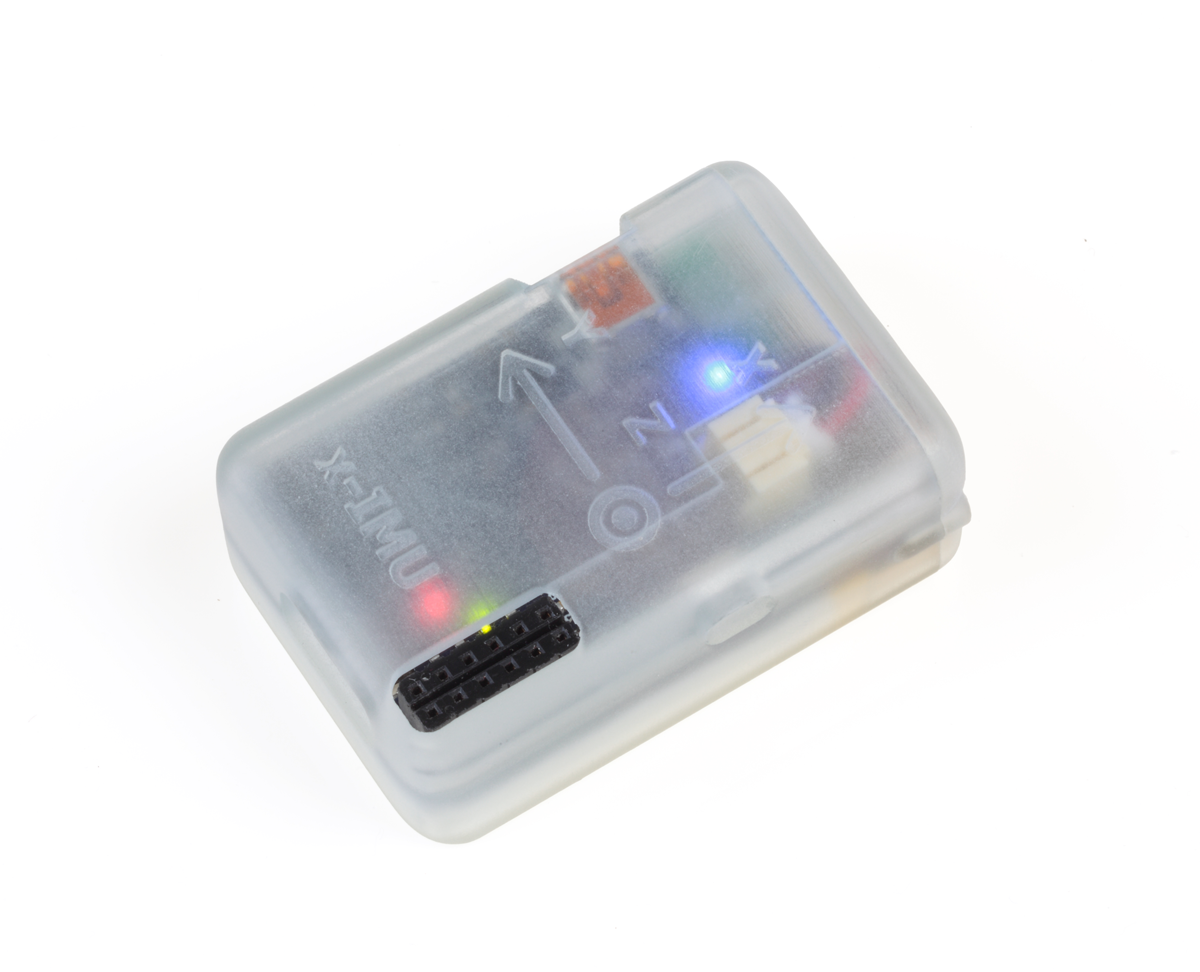
\includegraphics[width=0.5\textwidth]{graphics/ximu_plastic_housing_orthogonal_large.png}
		\caption{x-IMU and battery in plastic housing}
	\label{fig:ximu_plastic_housing_orthogonal_large}
\end{figure}

\begin{figure}[H]
    \begin{minipage}[b]{0.5\linewidth}
        \centering
            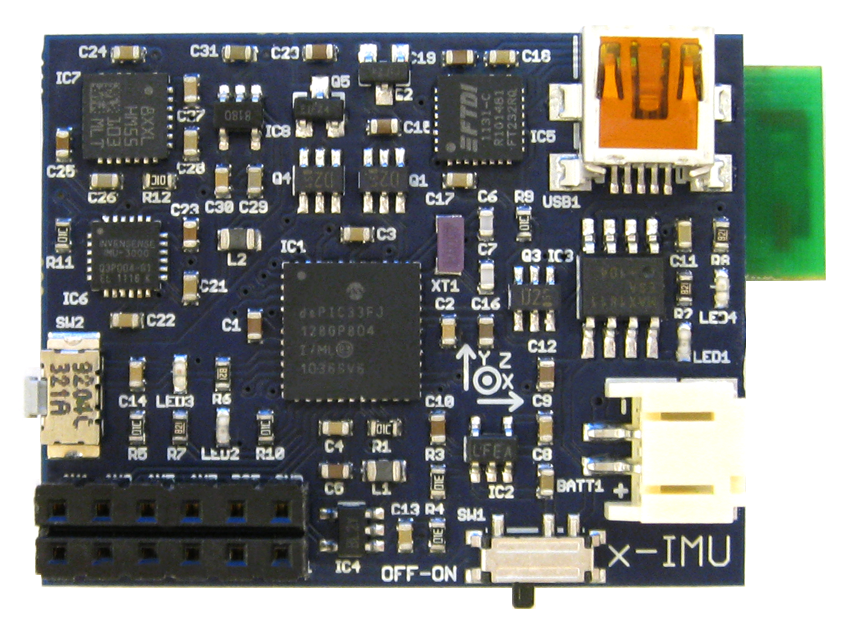
\includegraphics[width=0.8\textwidth]{graphics/ximu_pcb_top_large.png}
    		\caption{x-IMU top}
    	\label{fig:ximu_pcb_top_large}
    \end{minipage}
    \hspace{0.5cm}
    \begin{minipage}[b]{0.5\linewidth}
        \centering
            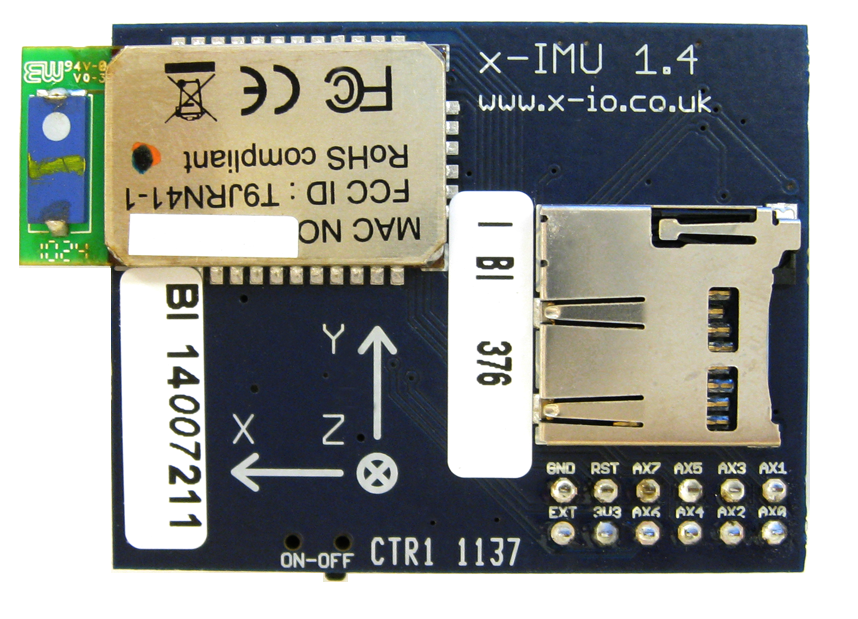
\includegraphics[width=0.8\textwidth]{graphics/ximu_pcb_bottom_large.png}
    		\caption{x-IMU bottom}
    	\label{fig:ximu_pcb_bottom_large}
    \end{minipage}
\end{figure}

%---------------------------------------------------------------------------------------------------
\subsection{Power switch}
\label{sec:PowerSwitch}

The power switch is used to switch the \hyperref[sec:BatteryAndCharging]{battery} and \hyperref[sec:USB]{USB} power on or off.  The battery and USB power is completely disconnected when the switch is in the \textit{off} position.  The x-IMU may be powered by an \hyperref[sec:ExternalSupply]{external supply} via the \hyperref[sec:AuxiliaryPort]{auxiliary port} if the power switch must be in the \textit{off} position.

%---------------------------------------------------------------------------------------------------
\subsection{Command button}
\label{sec:CommandButtonSum}

The command button that allows the execution of \hyperref[sec:Commands]{commands} while the x-IMU is operating as a standalone device.  See the \hyperref[sec:CommandButton]{command button} section for more information.

%---------------------------------------------------------------------------------------------------
\subsection{LEDs}
\label{sec:LEDs}

%------------------------------------------------
\subsubsection{Status LED (Green)}
\label{sec:StatusLEDGreen}

The green LED indicates the status of the x-IMU.  It will remain lit while the device is sampling and sending data and will otherwise be extinguished; for example, during the execution of some  \hyperref[sec:Commands]{commands}.  In \hyperref[sec:SleepMode]{sleep mode} the green LED will blink once every 3 seconds.  The green LED will flash rapidly while the on-board bootloader is active.

%------------------------------------------------
\subsubsection{SD card LED (Amber)}
\label{sec:SDCardLEDAmber}

The amber LED indicates \hyperref[sec:SDCard]{SD card} activity.  See the \hyperref[sec:SDCardLED]{SD card LED} section for more information.

%------------------------------------------------
\subsubsection{Bluetooth LED (Blue)}
\label{sec:BluetoothLEDBlue}

The blue LED indicates the state of the \hyperref[sec:Bluetooth]{Bluetooth} connection and power status.  See the \hyperref[sec:BluetoothLED]{Bluetooth LED} section for more information.

%------------------------------------------------
\subsubsection{Charging LED (Red)}
\label{sec:ChargingLEDRed}

The red LED indicates the \hyperref[sec:BatteryAndCharging]{charging state of the battery}.  The red LED will remain lit while the battery is charging and will be extinguished once the battery is charged.  See the \hyperref[sec:BatteryAndCharging]{battery and charging} section for more information.

%---------------------------------------------------------------------------------------------------
\subsection{USB socket}
\label{sec:USBSocket}

The USB mini-B socket is used to connect the x-IMU to a computer via a standard \textit{USB A to mini B (5 pin)} type cable.  See the \hyperref[sec:USB]{USB} section for more information.

%---------------------------------------------------------------------------------------------------
\subsection{Micro-SD card socket}
\label{sec:MicroSDCardSocket}

The micro SD card socket is used to log all data generated by the x-IMU to an \hyperref[sec:SDCard]{SD card}.  The x-IMU supports standard SD and SDHC cards formatted as either FAT16 or FAT32.  The file must be closed before the \hyperref[sec:SDCard]{SD card} is removed or the x-IMU switched of otherwise the current file will corrupt and data lost.  See the \hyperref[sec:SDCard]{SD card} section for more information.

%---------------------------------------------------------------------------------------------------
\subsection{Bluetooth module}
\label{sec:BluetoothModule}

The on-board Bluetooth module is used to connect the x-IMU to a Bluetooth host.  See the \hyperref[sec:Bluetooth]{Bluetooth} section for more information.

%---------------------------------------------------------------------------------------------------
\subsection{Battery connector}
\label{sec:BatteryConnector}

The on-board \hyperref[sec:BatteryAndCharging]{battery} connector allows the x-IMU to be powered by any single-cell Lithium Polymer (LiPo) battery.  The battery is automatically \hyperref[sec:BatteryAndCharging]{charged} while the x-IMU is connected to a \hyperref[sec:USB]{USB} host.  See the \hyperref[sec:BatteryAndCharging]{battery and charging} section for more information.

%---------------------------------------------------------------------------------------------------
\subsection{Auxiliary port header}
\label{sec:subAuxiliaryPortHeader}

The \hyperref[sec:AuxiliaryPort]{auxiliary port} that can be configured to one of many modes.  The auxiliary port connector is a $2\times6$, 2.54 mm pitch female header socket.  The socket pins include: ground, \hyperref[sec:ExternalSupply]{external power} input, 3.3 V output, hard reset and 8 I/O lines.  See the \hyperref[sec:AuxiliaryPort]{auxiliary port} section for more information.

%=====================================================================================================
\section{Software overview}
\label{sec:SoftwareOverview}

%The x-IMU software consists of the x-IMU GUI{} and x-IMU API{}.
%
%%---------------------------------------------------------------------------------------------------
%\subsection{Installing software and drivers}
%\label{sec:InstallingSoftwareAndDrivers}
%
%...
%
%%------------------------------------------------
%\subsubsection{Uninstalling software}
%\label{sec:UninstallingSoftware}
%
%May first need to uninstall x-IMU GUI before installing newer version.

%---------------------------------------------------------------------------------------------------
\subsection{x-IMU GUI}
\label{sec:xIMUGUI}

%The x-IMU GUI (Graphical User Interface) provides interface to all features and functionality of the x-IMU via the \hyperref[sec:xIMUAPI]{x-IMU API}. The x-IMU GUI is open source and so is intended to serve as a comprehensive template for those using the \hyperref[sec:xIMUAPI]{x-IMU API} to develop their own applications. Additional open source software examples using the \hyperref[sec:xIMUAPI]{x-IMU API} for various applications can be found on the \href{http://www.x-io.co.uk/node/10}{x-IMU Examples} webpage.
%
%\paragraph{Features}
%\begin{itemize}
%    \item View, edit and backup all x-IMU \hyperref[sec:Registers]{registers} and settings
%    \item Real-time 2D and 3D data graphics
%    \item Control panels for \hyperref[sec:AuxiliaryPort]{auxiliary port}
%    \item Data logger and file converter for exporting data; e.g. to MATLAB, Microsoft Excel, etc.
%    \item Magnetic calibration tools
%    \item Firmware bootloader to access new features in future x-IMU firmware versions
%\end{itemize}

%------------------------------------------------
\subsubsection{Tab page: Serial port}
\label{sec:TabPageSerialPort}

The serial port tab page is used to manage the USB or Bluetooth connection between the software and the x-IMU.  The USB and Bluetooth connections will each appear as a separate serial port; see the \hyperref[sec:USB]{USB} section and \hyperref[sec:Bluetooth]{Bluetooth} section for more information and how to find the serial port name assigned to each connection.

To connect to the x-IMU, the user first select the correct serial port name the x-IMU appears as in the \textit{Port name} drop down list.  If the name does not appear in the list, the user can either press the \textit{Refresh List} button to update the drop down list or type in the port name directly.  The \textit{Open Port} button may then be pressed to connect to the device.

\begin{figure}[H]
	\centering
		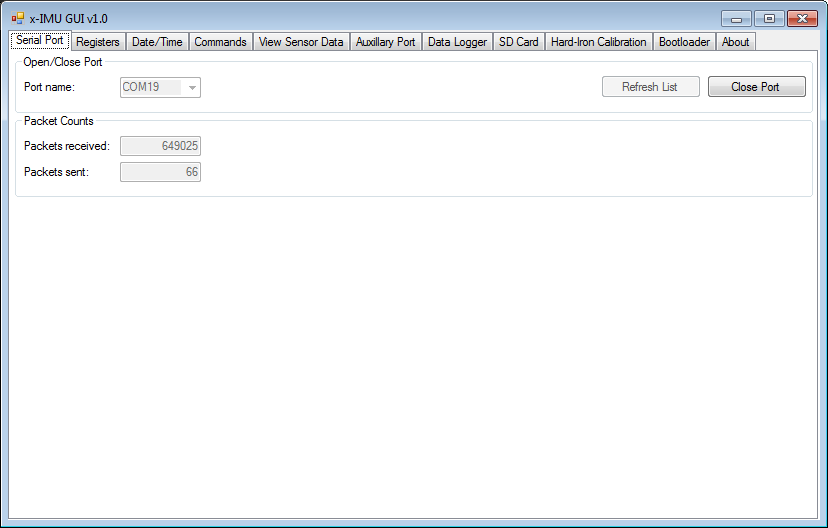
\includegraphics[width=0.8\textwidth]{graphics/GUI_tab_serial_port.png}
		\caption{x-IMU GUI{} serial port tab page}
	\label{fig:GUI_tab_serial_port}
\end{figure}

%------------------------------------------------
\subsubsection{Tab page: Registers}
\label{sec:TabPageRegisters}

The registers tab page allows the user to view, edit and back up all internal settings on the x-IMU; see the \hyperref[sec:Registers]{registers} section for more information on x-IMU registers.  All registers are organised into sections within a tree view where the end node of each branch is an individual register name and text box or drop down list containing the register value.  Register values that have been read directly from the x-IMU or loaded from file will appear as blue text.  Any registers values then edited will appear as red text.  A right click on any register will show the action menu.

To read all register on the x-IMU, the user should right click anywhere in the registers tab page and select \textit{Read all registers}.  The software will then read each register and update the values in the tree view.  Individual registers or groups of registers may be read by first selecting a register or group within the tree view and then selecting \textit{Read this register only} or \textit{Read all registers in this group only}.  Register values in the tree view may be written to the x-IMU using the \textit{Write all registers}, \textit{Write this register only} and \textit{Write all registers in this group only} options in the action menu.

\begin{figure}[H]
	\centering
		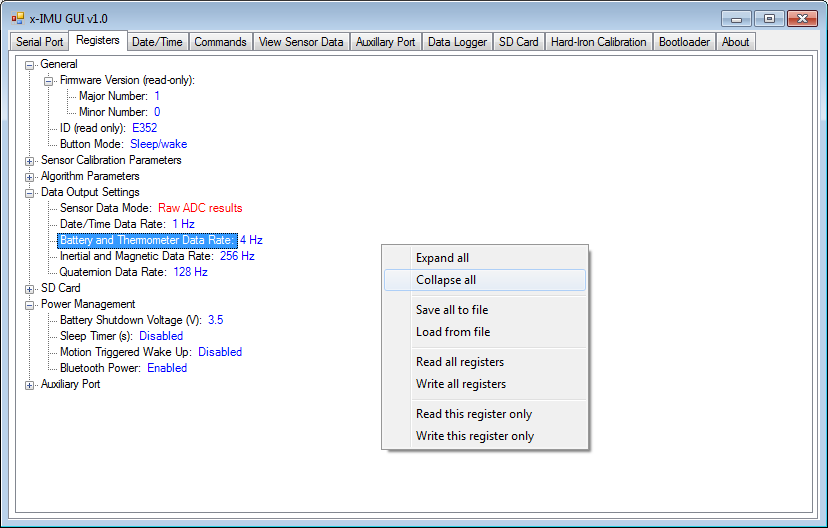
\includegraphics[width=0.8\textwidth]{graphics/GUI_tab_registers.png}
		\caption{x-IMU GUI{} registers tab page with (right click) action menu}
	\label{fig:GUI_tab_registers}
\end{figure}

%------------------------------------------------
\subsubsection{Tab page: Date/time}
\label{sec:TabPageDateTime}

The date/time tab page allows the user to view and set the date and time of the x-IMU's real-time clock and calendar.  The \textit{Received date/time} text box displays the date and time each time it is received from the x-IMU.  The \textit{Read Date/Time} button may be used to read the current date and time of the x-IMU; this is of use if date/time data rate has been disabled.  Pressing the \textit{Set Date/Time} button will set the x-IMU date and time equal to computer date and time.

\begin{figure}[H]
	\centering
		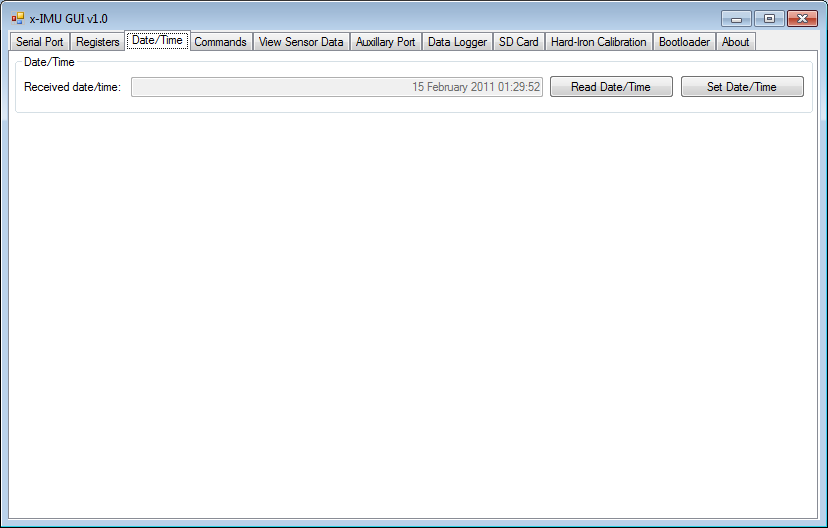
\includegraphics[width=0.8\textwidth]{graphics/GUI_tab_date_time.png}
		\caption{x-IMU GUI{} date/time tab page}
	\label{fig:GUI_tab_date_time}
\end{figure}

%------------------------------------------------
\subsubsection{Tab page: Commands}
\label{sec:TabPageCommands}

The commands tab page is used to send commands to the x-IMU.  See the \hyperref[sec:Commands]{commands} section for more information on individual commands.  Once the x-IMU has processed a command it will echo the command back and it will appear in a message box.  To suppress these message boxes, un-check the \textit{Display received command messages in message box} check box.

\begin{figure}[H]
	\centering
		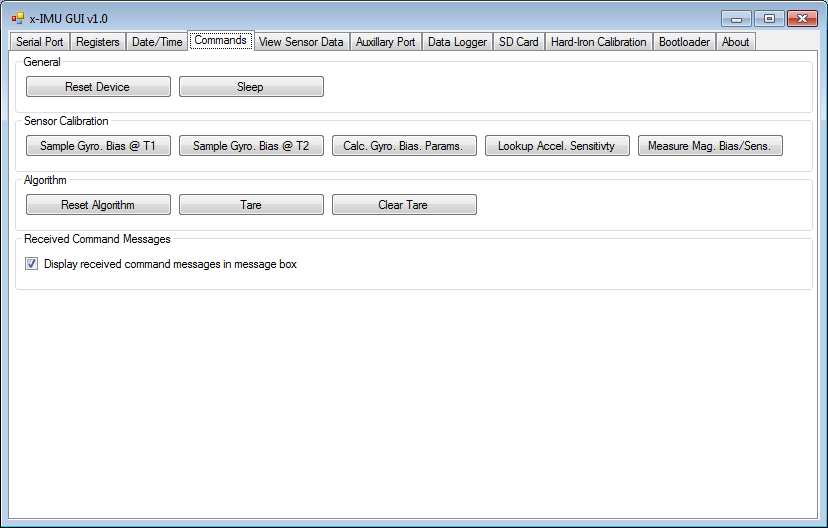
\includegraphics[width=0.8\textwidth]{graphics/GUI_tab_commands.png}
		\caption{x-IMU GUI{} date/time tab page}
	\label{fig:GUI_tab_commands}
\end{figure}

%------------------------------------------------
\subsubsection{Tab page: View sensor data}
\label{sec:TabPageViewSensorData}

The view sensor data tab page contains buttons to show or hide separate real-time data graphic windows for incoming x-IMU sensor data.

\begin{figure}[H]
	\centering
		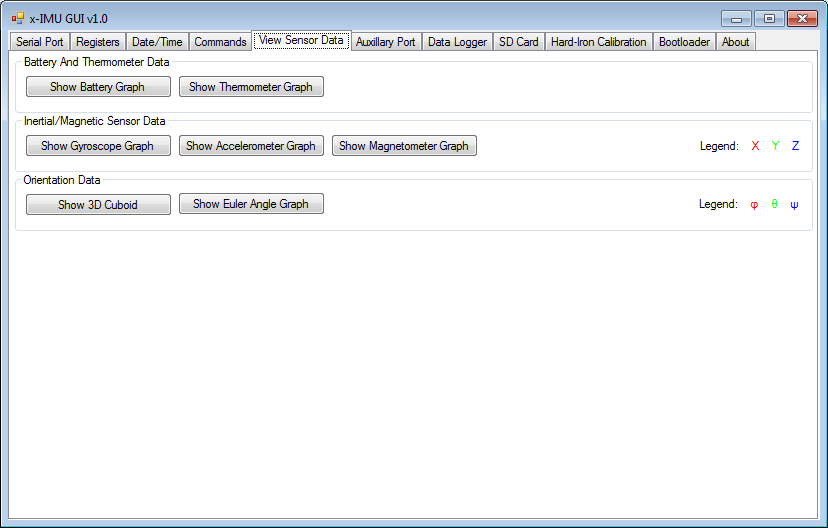
\includegraphics[width=0.8\textwidth]{graphics/GUI_tab_view_sensor_data.png}
		\caption{x-IMU GUI{} view sensor data tab page}
	\label{fig:GUI_tab_view_sensor_data}
\end{figure}

The data from individual sensors is displayed in real-time data graphs as seen in Figure \ref{fig:GUI_tab_view_sensor_data}.  The controls bar at the bottom of each graph allow the view and scaling to be adjusted.

\begin{figure}[H]
	\centering
		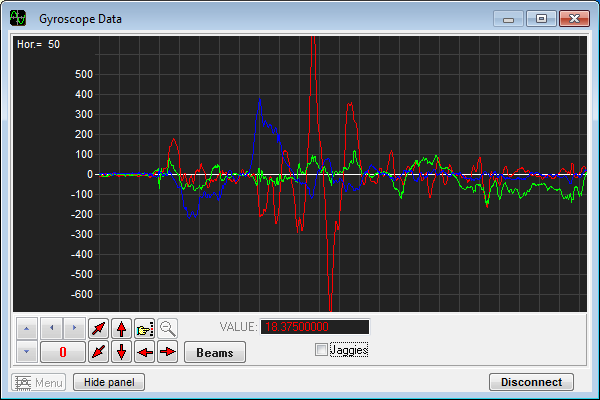
\includegraphics[width=0.5\textwidth]{graphics/GUI_gyroscope_graph.png}
		\caption{x-IMU GUI{} gyroscope data window}
	\label{fig:GUI_gyroscope_graph}
\end{figure}

Orientation data received may be displayed in a graph as ZYX Euler angles and displayed as the orientation of a 3D cuboid as seen in figure \ref{fig:GUI_3D_cuboid}.  The cuboid is displayed in a screen coordinate frame where the x-axis is aligned to the width of the screen (left to right), the z-axis aligned to the height (bottom to top) and the y-axis projects into the screen.  To align the motion of the physical x-IMU and 3D cuboid displayed on the screen, the user should first align the axes of the physical x-IMU to the screen coordinate frame and then use the \textit{\hyperref[sec:AlgorithmTare]{algorithm tare}} command.

\begin{figure}[H]
	\centering
		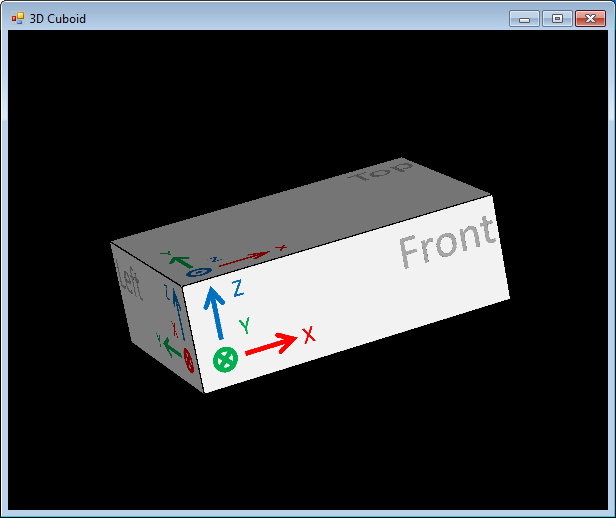
\includegraphics[width=0.5\textwidth]{graphics/GUI_3D_cuboid.png}
		\caption{x-IMU GUI{} 3D cuboid window}
	\label{fig:GUI_3D_cuboid}
\end{figure}

%------------------------------------------------
\subsubsection{Tab page:  Auxiliary port}
\label{sec:TabPageAuxillaryPort}

The auxiliary port tab page contains buttons to show or hide individual control windows for the different modes of the auxiliary port.

\begin{figure}[H]
	\centering
		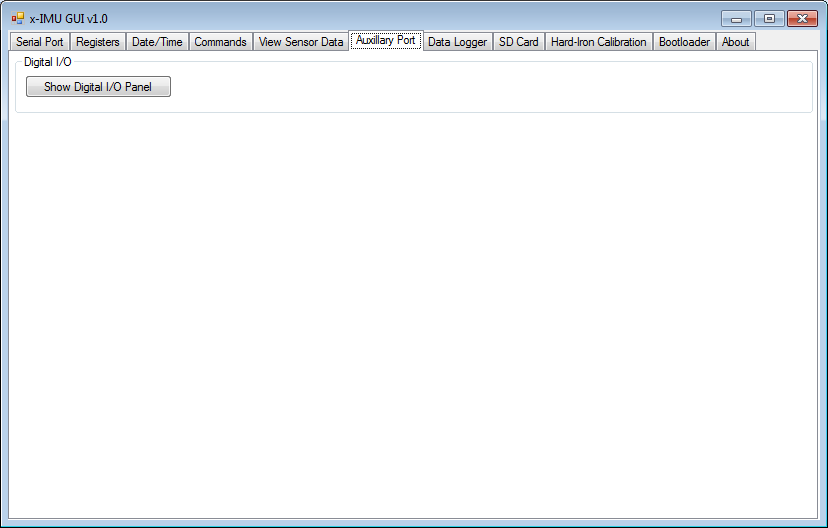
\includegraphics[width=0.8\textwidth]{graphics/GUI_tab_auxiliary_port.png}
		\caption{x-IMU GUI{} auxiliary port tab page}
	\label{fig:GUI_tab_auxiliary_port}
\end{figure}

\paragraph{Digital I/O control panel}
\label{sec:DigitalIOControlPanel}
The digital I/O control panel displays the state and mode of each channel of the auxiliary port when in digital I/O mode as shown in figure \ref{fig:GUI_digital_IO_control_panel}.  Each channel is represented by a check box.  If the channel mode is output then the check box is enabled and may be checked or un-checked to set the channel high or low respectively.  If the channel is an input the check box is disabled and will be checked or un-checked if the channel is high or low respectively.

\begin{figure}[H]
	\centering
		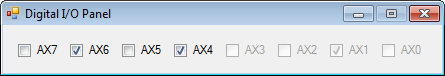
\includegraphics[width=0.4\textwidth]{graphics/GUI_digital_IO_control_panel.png}
		\caption{x-IMU GUI{} digital I/O control panel}
	\label{fig:GUI_digital_IO_control_panel}
\end{figure}

%------------------------------------------------
\subsubsection{Tab page:  Data logger}
\label{sec:TabPageDataLogger}

The data logger tab allows the user to log incoming real-time data to file.  These files may be imported to user software such as Microsoft Excel and MATLAB.  The user may select the location and first part of the file name in the \textit{File path} text box.  This file name will be extended with an appropriate description and extension when the individual data files are created.  For example, if a file name of \verb=myFile= is specified, Euler angle and date/time data will be saved to \verb=myFile_EulerAngles.csv= and \verb=myFile_DateTime.txt=.

\begin{figure}[H]
	\centering
		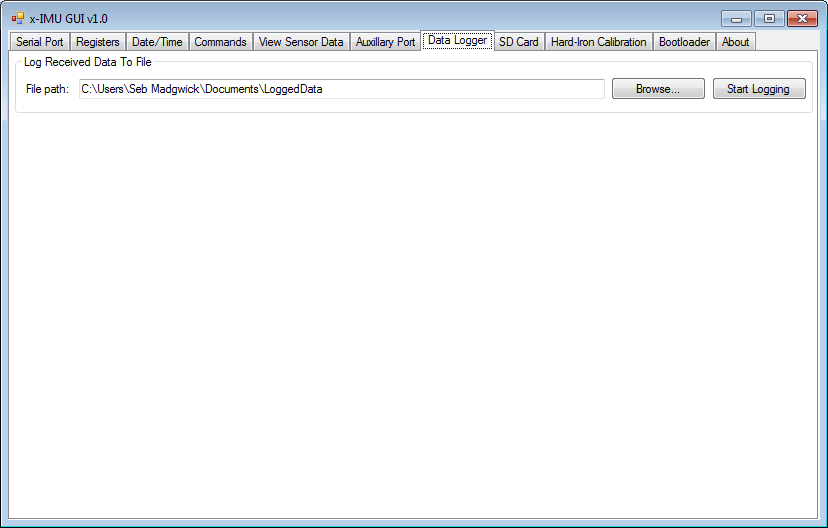
\includegraphics[width=0.8\textwidth]{graphics/GUI_tab_data_logger.png}
		\caption{x-IMU GUI{} data logger tab page}
	\label{fig:GUI_tab_data_logger}
\end{figure}

The \textit{Start/Stop Logging} button is used to start and stop the data logger.  When logging is stopped, a report window will be presented detailing the number of each type of packet logged and the specific data files created; as shown in figure \ref{fig:GUI_data_logger_report}.

\begin{figure}[H]
	\centering
		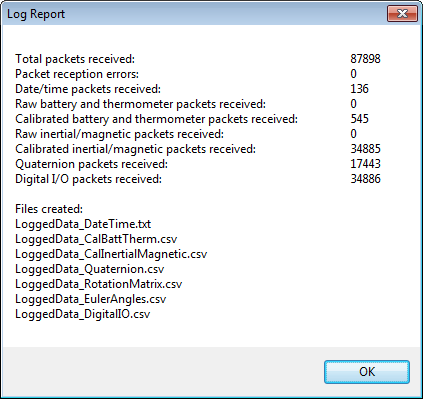
\includegraphics[width=0.4\textwidth]{graphics/GUI_data_logger_report.png}
		\caption{x-IMU GUI{} data logger report}
	\label{fig:GUI_data_logger_report}
\end{figure}

%------------------------------------------------
\subsubsection{Tab page:  SD card}
\label{sec:TabPageSDCard}

The SD card tab page allows the user to convert binary files (\verb=.bin=) saved to the SD card in to readable data files.  These files may be imported to user software such as Microsoft Excel and MATLAB.  The location and file name must be specified in the \textit{File path} text box.  The file conversion will start when the \textit{Convert} button is clicked.  This process occurs in the background and may take a while if a large binary file is specified.

\begin{figure}[H]
	\centering
		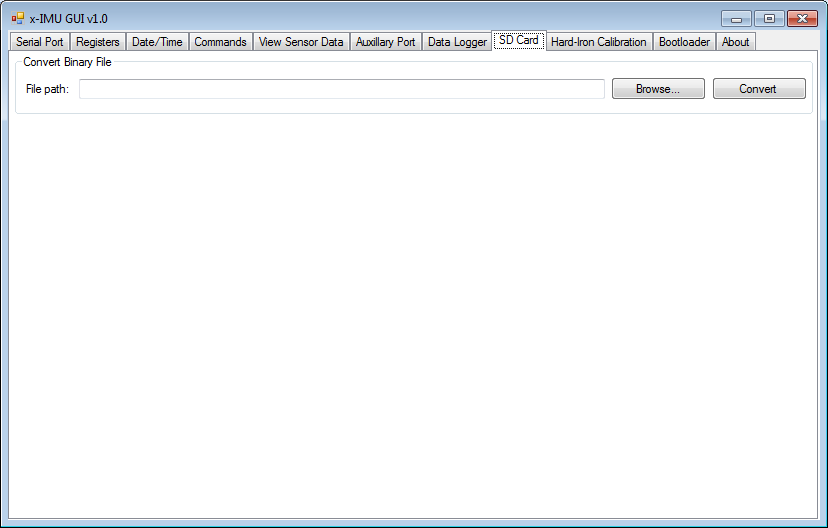
\includegraphics[width=0.8\textwidth]{graphics/GUI_tab_SD_card.png}
		\caption{x-IMU GUI{} SD card tab page}
	\label{fig:GUI_tab_SD_card}
\end{figure}

Once the conversion is complete, a report window will be presented detailing the number of each type of packet read and the specific data files created; as shown in figure \ref{fig:GUI_conversion_report}.

\begin{figure}[H]
	\centering
		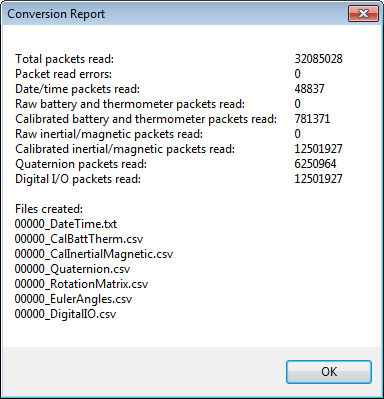
\includegraphics[width=0.35\textwidth]{graphics/GUI_conversion_report.png}
		\caption{x-IMU GUI{} binary file conversion report}
	\label{fig:GUI_conversion_report}
\end{figure}

%------------------------------------------------
\subsubsection{Tab page:  Hard-iron calibration}
\label{sec:TabPageHardIronCalibration}

The hard-iron calibration tab page provides all the functionality required for the user to calibrate for hard-iron interferences affecting the x-IMU.  It is necessary to re-calibrate hard-iron parameters whenever the x-IMU's magnetic characteristics are changed; for example, when the x-IMU if fitted to a battery or mounting that includes ferromagnetic elements.  The 3 group boxes, \textit{Step 1 - Clear Hard-Iron Bias Registers}, \textit{Step 2 - Collect Hard-Iron Calibration Dataset} and \textit{Step 3 - Run Hard-Iron Calibration Algorithm} represent the 3 steps that must be performed in order.  See the \hyperref[sec:MagnetometerHardIronCalibration]{magnetometer hard-iron calibration} section for more information.

\begin{figure}[H]
	\centering
		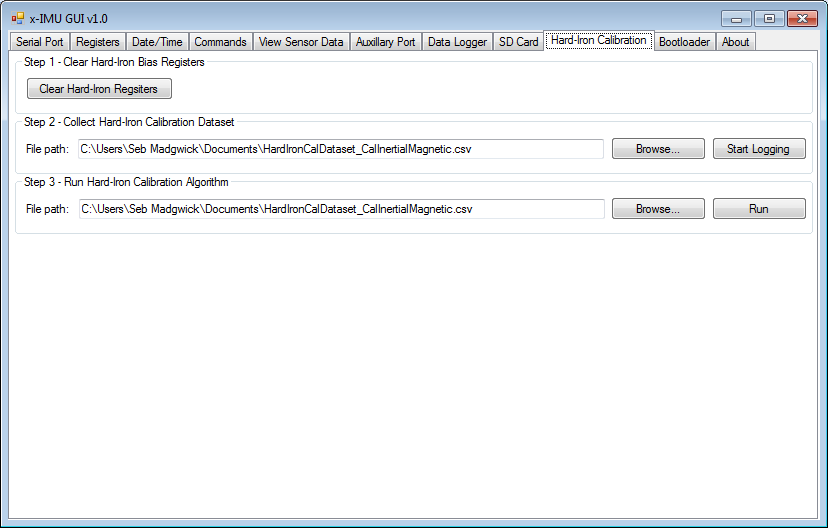
\includegraphics[width=0.8\textwidth]{graphics/GUI_tab_hard_iron_calibration.png}
		\caption{x-IMU GUI{} hard-iron calibration tab page}
	\label{fig:GUI_tab_hard_iron_calibration}
\end{figure}

%%------------------------------------------------
%\subsubsection{Tab page: Upload firmware}
%\label{sec:TabPageUploadFirmware}
%
%The bootloader tab page allows the x-IMU firmware to be updated.  The bootloader may only be used while the x-IMU is connected via USB and the serial port closed.  See the bootloader section (\ref{sec:Bootloader}) for more information.
%
%\begin{figure}[H]
%	\centering
%		\includegraphics[width=0.8\textwidth]{graphics/GUI_tab_bootloader.png}
%		\caption{x-IMU GUI{} bootloader tab page}
%	\label{fig:GUI_tab_bootloader}
%\end{figure}

%---------------------------------------------------------------------------------------------------
\subsection{x-IMU API}
\label{sec:xIMUAPI}

The x-IMU API{} (Application Programming Interface) is a code library that contains all the classes, data structures and methods required to interface to all features and functionality of the x-IMU.  The x-IMU API{} is an open source project written in C\# and targets Microsoft .NET 3.5.  Documentation for use of the API is represented by the XML comments throughout the source code which is accessed automatically by Visual Studio's IntelliSense.  The open source x-IMU GUI{} serves as a comprehensive template for use of all features of the x-IMU API{}.  See the \href{http://www.x-io.co.uk/node/10}{x-IMU Examples} web page for further open-source examples and applications.

%=====================================================================================================
% USB
%=====================================================================================================
\section{USB}
\label{sec:USB}

The x-IMU streams all communication data simultaneously and identically via USB, \hyperref[sec:Bluetooth]{Bluetooth} and to a file on the \hyperref[sec:SDCard]{SD card}.  The USB and Bluetooth connections are also be used to send \hyperref[sec:Commands]{commands}, read/write \hyperref[sec:Registers]{registers} and control the \hyperref[sec:AuxiliaryPort]{auxiliary port} outputs from the host software application.  As both USB and Bluetooth connections appear as serial ports, use of either communication channel is identical.

The x-IMU can be connected to a computer via a standard USB \textit{A to mini B (5 pin)} type cable.  The on-board FTDI USB chip is widely used USB interface with \href{http://www.ftdichip.com/Drivers/VCP.htm}{drivers available} for Windows, Mac OS X and Linux.  Once the drivers have been \hyperref[sec:InstallingUSBDrivers]{installed} and the x-IMU connected to the computer, the x-IMU will appear as a serial port and be assigned an available port name; for example \textit{COM2}.  The computer may then communicate with the x-IMU by opening this serial port.  This is achieved via the \textit{\hyperref[sec:TabPageSerialPort]{serial port}} tab page of the \hyperref[sec:xIMUGUI]{x-IMU GUI}.

The USB connection is a reliable communication channel that cannot be comprised by user settings; the x-IMU will not enter \hyperref[sec:SleepMode]{sleep mode} due to the \hyperref[sec:SleepTimer]{sleep timer} or \hyperref[sec:LowBatteryVoltageDetection]{low battery voltage detection} while the USB is connected.  The USB connection can be used to power the x-IMU and is used by the on-board \hyperref[sec:BatteryAndCharging]{charging} circuit to charge the battery if connected.  The on-board USB interface is powered directly by the USB connection so that the x-IMU will remain detectable and the serial port may be held open by the computer even while the x-IMU is switched off or in \hyperref[sec:SleepMode]{sleep mode}.

%---------------------------------------------------------------------------------------------------
\subsection{Installing USB drivers}
\label{sec:InstallingUSBDrivers}

The Windows USB drivers can be downloaded from the \href{http://www.x-io.co.uk/node/9}{x-IMU webpage}.  Drivers for other operating systems are available of the \href{http://www.ftdichip.com/Drivers/VCP.htm}{FTDI website}.  To install the Windows drivers, simply run the \verb=.exe= file.  This will automatically detect specific Windows operating system being used and install the correct drivers.  Once the drivers have been installed and the x-IMU connected to the computer, the x-IMU will appear as a serial port and be assigned an available port name; for example \textit{COM2}.  The port name assigned to the x-IMU USB connection can be confirmed at any time by viewing the computer's \textit{Ports} in Windows device manager; as shown in Figure \ref{fig:USBportName}.

\begin{figure}[H]
	\centering
		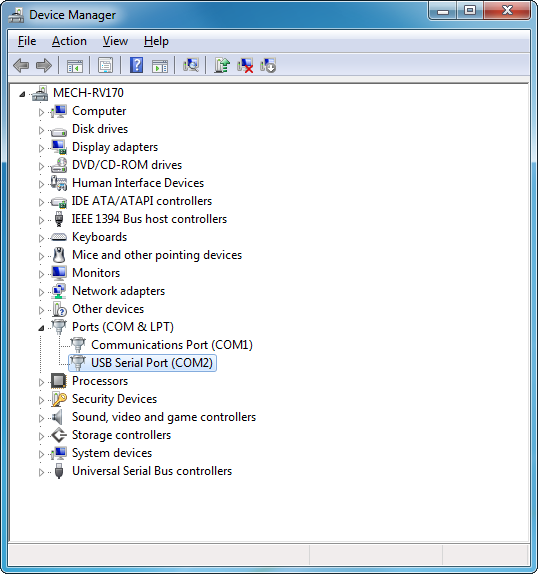
\includegraphics[width=0.5\textwidth]{graphics/USBportName.png}
		\caption{Confirming the port name assigned to the x-IMU USB connection}
	\label{fig:USBportName}
\end{figure}

\paragraph{Windows serial mouse bug}
\label{sec:WindowsSerialMouseBug}
Windows may misinterpret the constant stream of data from the x-IMU as the behaviour of a serial mouse when the x-IMU USB is connected.  This will lead to the mouse cursor being `hi-jacked' by apparent random behaviour.  If this happens the x-IMU should be unplugged and reconnected while switched off or in \hyperref[sec:SleepMode]{sleep mode} for the first few seconds of connection.  The `hi-jacked' activity may leave the mouse buttons disabled which can be undone by entering and then leaving the \textit{Ctrl + Alt + Del} screen.

%---------------------------------------------------------------------------------------------------
\subsection{USB bandwidth}
\label{sec:USBBandwidth}

It is possible for the user to define \hyperref[sec:BatteryAndThermometerDataOutputRate]{data output rates} so that the amount of data being generated by the x-IMU exceeds the bandwidth of a communication channel.  If the USB bandwidth is exceed, the USB transmit buffer will overrun and some data will be lost.  When this happens a \textit{\hyperref[sec:USBTransmitBufferOverrun]{USB transmit buffer overrun}} error will be generated.  As this error is sent immediately after the buffer has overrun, the error will be successfully transmitted.  This error can be avoided by reducing the \hyperref[sec:BatteryAndThermometerDataOutputRate]{data output rates}.

All data sent to the x-IMU via USB is buffered in the USB receive buffer before being processed.  The time required to process the received data is dependent on the data.  If data is sent to the x-IMU via USB at a rate at a rate greater than it can be processed then the receive buffer will overflow and some data will be lost.  When this happens a \textit{\hyperref[sec:USBReceiveBufferOverrun]{USB receive buffer overrun}} error will be generated.

%=====================================================================================================
% Bluetooth
%=====================================================================================================
\section{Bluetooth}
\label{sec:Bluetooth}

The x-IMU streams all communication data simultaneously and identically via \hyperref[sec:USB]{USB}, Bluetooth and to a file on the \hyperref[sec:SDCard]{SD card}.  The USB and Bluetooth connections are also be used to send \hyperref[sec:Commands]{commands}, read/write \hyperref[sec:Registers]{registers} and control the \hyperref[sec:AuxiliaryPort]{auxiliary port} outputs from the host software application.  As both USB and Bluetooth connections appear as serial ports, use of either communication channel is identical.

The on-board Bluetooth radio is a class I device with a maximum range of 100 m.  The radio uses the Serial Port Profile (SPP) to enable connection to any Bluetooth host without the need to install specific drivers.  Once \hyperref[sec:PairingTheXIMUWithABluetoothHost]{paired with a Bluetooth host}, the x-IMU will appear as a serial port and be assigned an available port name; for example \textit{COM3}.  The computer connects to the x-IMU via Bluetooth by opening this serial port.  This is achieved via the \textit{\hyperref[sec:TabPageSerialPort]{Serial Port}} tab page of the \hyperref[sec:xIMUGUI]{x-IMU GUI}.  The Bluetooth connection will be lost when the x-IMU is switch off, enters \hyperref[sec:SleepMode]{sleep mode} or is out of range.  The connection status of the x-IMU is indicated by the \hyperref[sec:BluetoothLED]{Bluetooth LED}.  The Bluetooth radio can be completely disabled by the user via the \textit{\hyperref[sec:BluetoothPower]{Bluetooth power}} register to \hyperref[sec:TipsForMinimisingPowerConsumption]{reduce power consumption}.

%---------------------------------------------------------------------------------------------------
\subsection{Pairing the x-IMU with a Bluetooth host}
\label{sec:PairingTheXIMUWithABluetoothHost}

As with any Bluetooth device, the x-IMU must first be paired with the host computer before a Bluetooth connection can be made.  This pairing process is the same for all Bluetooth devices and will be familiar those who have used other Bluetooth devices such as printers or mobile phones.

To pair the x-IMU with a host computer, the host computer's Bluetooth must be enabled and the x-IMU must be switched on and the \hyperref[sec:BluetoothPower]{Bluetooth power} enabled so that the \hyperref[sec:BluetoothLED]{Bluetooth LED} is flashing.  The user may then use the host computer to search for and the x-IMU to be paired with the computer.  The x-IMU will appear with the name ``x-IMU-ABCD'' where the characters ``ABCD'' are the \textit{\hyperref[sec:DeviceID]{device ID}} of the x-IMU.  For example,  Figure \ref{fig:AddBluetoothDeviceSearch} shows how this is done in Windows 7 having right clicked the Bluetooth icon the task bar.

\begin{figure}[H]
	\centering
		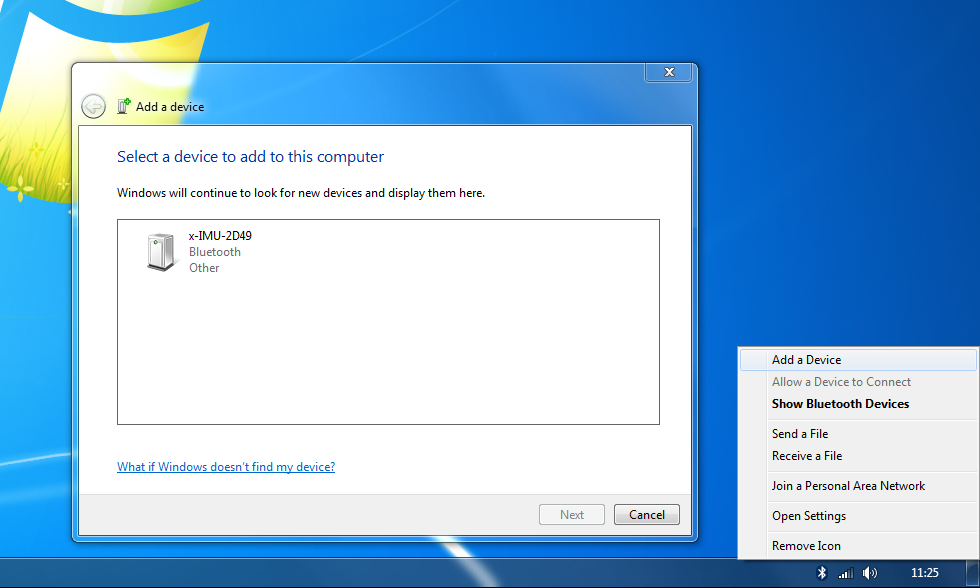
\includegraphics[width=0.7\textwidth]{graphics/AddBluetoothDeviceSearch.png}
		\caption{Searching for the x-IMU as a new Bluetooth device in Windows 7}
	\label{fig:AddBluetoothDeviceSearch}
\end{figure}

Once the x-IMU has been found by the host computer, it can be added.  This will require the user to enter the x-IMU's Bluetooth pass code: ``1234''.  The x-IMU Bluetooth pairing will be assigned an available serial port name by the host computer; for example \textit{COM3}.  For example, Figure \ref{fig:AddBluetoothDevicePasscode} shows this being done in Windows 7.

\begin{figure}[H]
	\centering
		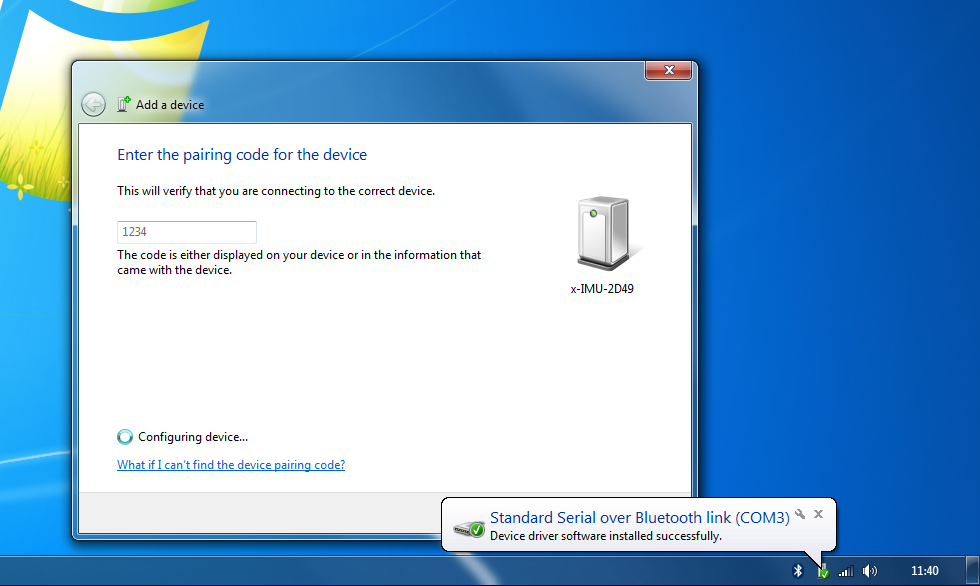
\includegraphics[width=0.7\textwidth]{graphics/AddBluetoothDevicePasscode.png}
		\caption{Adding the x-IMU as a new Bluetooth device in Windows 7}
	\label{fig:AddBluetoothDevicePasscode}
\end{figure}

The port name assigned to the x-IMU Bluetooth pairing can be confirmed at any time by viewing the services of the x-IMU.  For example, Figure \ref{fig:BluetoothServices} shows how this is done in Windows 7 having right clicked the x-IMU Bluetooth device icon.

\begin{figure}[H]
	\centering
		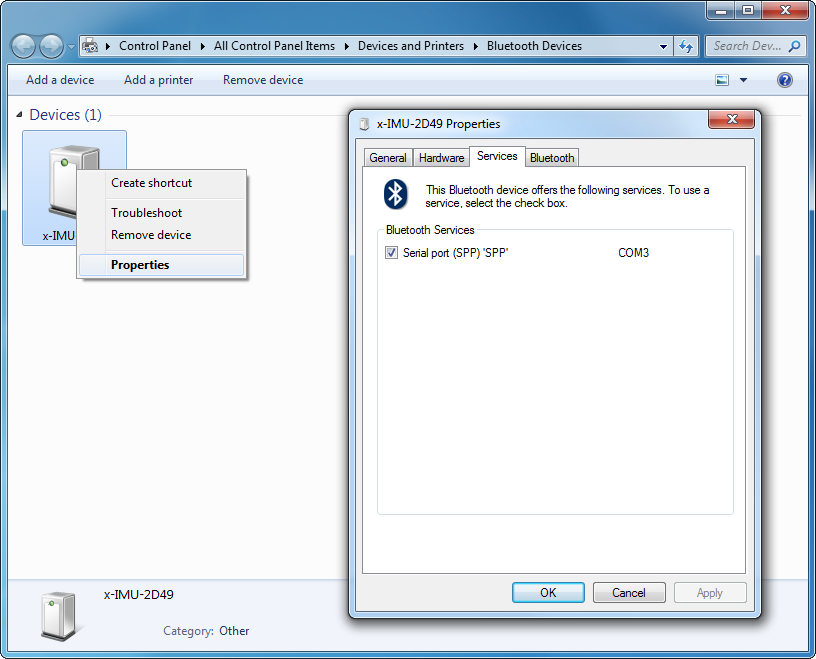
\includegraphics[width=0.6\textwidth]{graphics/BluetoothServices.png}
		\caption{Confirming the port name assigned to the x-IMU Bluetooth pairing}
	\label{fig:BluetoothServices}
\end{figure}

%---------------------------------------------------------------------------------------------------
\subsection{Bluetooth LED}
\label{sec:BluetoothLED}

The blue Bluetooth LED indicates the Bluetooth radio state.  The LED behaviour and associated Bluetooth radio states are detailed in table \ref{tab:BluetoothLEDstates}.

\begin{table}[H]
	\centering
		\begin{tabular}{l  l}
		\hline
		LED behaviour		&	Bluetooth state\\
		\hline
		Off							& Switched off.  Power to the radio is completely disconnected\\
		Flashing (1 Hz)	& Fully powered and discoverable\\
		On							& Fully powered and connected\\
		\hline
		\end{tabular}
		\caption{Bluetooth LED states}
	\label{tab:BluetoothLEDstates}
\end{table}

%---------------------------------------------------------------------------------------------------
\subsection{Bluetooth bandwidth}
\label{sec:BluetoothBandwidth}

It is possible for the user to define \hyperref[sec:BatteryAndThermometerDataOutputRate]{data output rates} so that the amount of data being generated by the x-IMU exceeds the bandwidth of a communication channel.  If the Bluetooth bandwidth is exceed, the Bluetooth transmit buffer will overrun and some data will be lost.  When this happens a \textit{\hyperref[sec:BluetoothTransmitBufferOverrun]{Bluetooth transmit buffer overrun}} error will be generated.  As this error is sent immediately after the buffer has overrun, the error will be successfully transmitted.  This error can be avoided by reducing the \hyperref[sec:BatteryAndThermometerDataOutputRate]{data output rates}.

All data sent to the x-IMU via Bluetooth is buffered in the Bluetooth receive buffer before being processed.  The time required to process the received data is dependent on the data.  If data is sent to the x-IMU via Bluetooth at a rate at a rate greater than it can be processed then the receive buffer will overflow and some data will be lost.  When this happens a \textit{\hyperref[sec:BluetoothReceiveBufferOverrun]{Bluetooth receive buffer overrun}} error will be generated.

%---------------------------------------------------------------------------------------------------
\subsection{Optimising Bluetooth performance}
\label{sec:OptimisingBluetoothPerformance}

The practical range and quality of the Bluetooth connection are dependent on a number of factors.  A poor Bluetooth connection will be unable to handle higher data output rates and so result in missing data and \textit{\hyperref[sec:BluetoothTransmitBufferOverrun]{Bluetooth transmit buffer overrun}} errors.  The use of lower \hyperref[sec:BatteryAndThermometerDataOutputRate]{data output rates} can help achieve a more reliable Bluetooth communication channel.

The x-IMU uses a class I Bluetooth radio which represents a maximum range of 100 m.  However, the practical performance is also limited by computer's Bluetooth class; for example a class II Bluetooth dongle (representing a range of 10 m) will limit the x-IMU's operating range to 10 m.  Performance also varies between Bluetooth dongle brands; a dongle from a  reputable brand may be expected to perform better than a low-cost, `budget' product.  Bluetooth is a radio system and so the location of the antennae (usually built into the dongle) should be given consideration.  For example, a miniature Bluetooth dongle plugged in to the back a desktop PC can be expected to achieve worse performance than if the dongle was fixed to a front USB port with line-of-sight to the x-IMU.

%---------------------------------------------------------------------------------------------------
\subsection{Connecting to multiple x-IMUs via Bluetooth}
\label{sec:ConnectingToMultipleXIMUsViaBluetooth}

A single Bluetooth host/master (e.g. Bluetooth dongle) can connect to up to 7 Bluetooth slaves (e.g. x-IMUs) simultaneously.  Each x-IMU is assigned a separate serial port name and operates independently.  However, the bandwidth will be limited to that of the single Bluetooth host.

%=====================================================================================================
\section{SD card}
\label{sec:SDCard}

The x-IMU streams all communication data simultaneously and identically via \hyperref[sec:USB]{USB}, \hyperref[sec:Bluetooth]{Bluetooth} and to a file on the SD card.  The SD card may therefore be used in conjunction with the USB and/or Bluetooth or as the sole communication channel allowing the x-IMU to function as a standalone data logger.  Data is logged to the SD card on separate files binary files that are automatically created each time the x-IMU is switched on, reset or wakes up.  Logging is only then stopped once the x-IMU is reset or enters \hyperref[sec:SleepMode]{sleep mode}.

The binary files (\verb=.bin=) created may be read form the SD card on to any PC and then converted to individual Comma Separated Variable (\verb=.csv=) files using via the x-IMU GUI{} \textit{\hyperref[sec:TabPageSDCard]{SD Card}} tab page.  Alternatively the \href{http://www.x-io.co.uk/node/10#sd_card_binary_file_converter}{x-IMU Binary File Converter} may be used for command-line-based or automated conversion of multiple files.  Converted CSV and text files can be directly imported into programmes such as MATLAB and Microsoft Excel.  The x-IMU MATLAB Library includes all the tools required to import, structure and plot x-IMU data.

The x-IMU supports standard SD cards and SDHC cards\footnote{The x-IMU has known compatibility issues with counterfeit SDHC cards.  It is recommended that you only use genuine products from a reputable brand.}.  Cards may be formatted as FAT16 (usually cards equal or less than 2 GB) and FAT32 (for card greater than 2 GB).  For reliable performance it is recommended that the SD card is formatted prior to each use.

%---------------------------------------------------------------------------------------------------
\subsection{Creating and closing files}
\label{sec:CreatingAndClosingFiles}

The x-IMU automatically creates a new file on the SD card each time the x-IMU is switched on, reset or wakes up.  If an SD card is not accessible at this point, the x-IMU will not create a file and the SD card will not be used.  The new file name is created as the 5 digit number stored in the \textit{\hyperref[sec:SDCardNewFileName]{SD card new file name}} register.  For example, \verb=00000.bin=.  The number stored in this register is automatically incremented each time a new file is created.  This ensures that each file created by the x-IMU is given a unique file name until the maximum file name of \verb=65535.bin= is reached, the file name will then automatically reset to \verb=00000.bin= and start again.  The user may also edit this value to any number by writing to the \hyperref[sec:SDCardNewFileName]{register}.  If the x-IMU attempts to create a file name that already exists on the SD card, the x-IMU automatically increment the file name and try again.  If all file names have been used, the x-IMU will not create a file and the SD card will not be used.

Files must be closed before the SD card is removed or the x-IMU switched off otherwise the file will be corrupted and all data written to the file will be lost.  The file is automatically closed when the x-IMU is reset or enters \hyperref[sec:SleepMode]{sleep mode}.  Users wishing to frequently remove the SD card may wish to have the \hyperref[sec:CommandButton]{command button} configured in \textit{sleep/wake} mode.

%---------------------------------------------------------------------------------------------------
\subsection{SD card LED}
\label{sec:SDCardLED}

The amber SD card LED indicates SD card activity.  The LED remains lit each time a burst of data is written to the SD card.  If the user low defines data output rates then the LED will blink infrequently, high data output rates will mean the LED will flash rapidly.  In this way the SD card LED provides an indication of \hyperref[sec:SDCardBandwidth]{SD card bandwidth} performance.

%---------------------------------------------------------------------------------------------------
\subsection{SD card bandwidth}
\label{sec:SDCardBandwidth}

It is possible for the user to define \hyperref[sec:BatteryAndThermometerDataOutputRate]{data output rates} so that the amount of data being generated by the x-IMU exceeds the bandwidth of a communication channel.  The SD card bandwidth is greater than the USB and Bluetooth bandwidth and so the SD card may still provide reliable data logging when the USB or Bluetooth channel bandwidth is exceeded.  If the SD card bandwidth is exceed, the SD card buffer will overrun and some data will be lost.  When this happens an \textit{\hyperref[sec:SDCardWriteBufferOverrun]{SD card write buffer overrun}} error will be generated.  This \textit{error} packet is sent immediately after the buffer has overrun so that the error will always be successfully logged to the SD card.  This error can be avoided by reducing the \hyperref[sec:BatteryAndThermometerDataOutputRate]{data output rates}.  The \hyperref[sec:SDCardLED]{SD card LED} may be used to provides an indication of SD card bandwidth performance while access to errors is not available.

The effective bandwidth of SD card is varies between different SD card brands and may decrease significantly if the SD card becomes fragmented.  It is therefore recommended that the SD card is formatted prior to each use.

%---------------------------------------------------------------------------------------------------
\subsection{Magnetic distortions from the SD card socket}
\label{sec:MagneticDistortionsFromTheSDCardSocket}

The SD card socket contains a ferromagnetic mechanism that may distort \hyperref[sec:Magnetometer]{magnetometer} measurements in different ways dependant on whether an SD card is inserted or not.  These distortions are removed from measurements through \hyperref[sec:MagnetometerHardIronCalibration]{hard-iron calibration}.  Each x-IMU is calibrated and supplied with a dummy SD card that may be used to ensure constant SD card socket magnetic characteristics.

%=====================================================================================================
\section{Command button}
\label{sec:CommandButton}

The x-IMU features a configurable command button that allows the execution of \hyperref[sec:Commands]{commands} while the x-IMU is operating as a standalone device.  The \hyperref[sec:CommandButtonModes]{command button modes} are detailed below.  Only \textit{reset} and \textit{sleep/wake up} modes remain active while the x-IMU is in \hyperref[sec:SleepMode]{sleep mode}.  The command button is also used to confirm the \hyperref[sec:FactoryReset]{factory reset} command.

\paragraph{Command button modes}
\label{sec:CommandButtonModes}

\begin{itemize}
  \item \textit{Disabled}
  \item \textit{\hyperref[sec:Reset]{Reset}} command
  \item \textit{\hyperref[sec:Sleep]{Sleep}/wake up}
  \item \textit{\hyperref[sec:AlgorithmInitialise]{Algorithm initialise}} command
  \item \textit{\hyperref[sec:AlgorithmTare]{Algorithm tare}} command
  \item \textit{\hyperref[sec:AlgorithmInitialiseThenTare]{Algorithm initialise then tare}} command
\end{itemize}

%=====================================================================================================
\section{Real-time clock and calendar}
\label{sec:RealTimeClockAndCalendar}

The on-board real-time clock and calendar provides accurate measurement of the date and time and is pre-programmed to account for leap-years between the year 2000 and 2099.  The real-time clock and calendar data can be viewed and synchronised with the computer clock using the \hyperref[sec:xIMUGUI]{x-IMU} via the \textit{\hyperref[sec:TabPageDateTime]{Date/Time}} tab page.

The real-time clock and calendar data is provided by the x-IMU in the \textit{write date/time data} packets.  The data output rate of these packets may be set to \textit{disabled}, 1 Hz, 2 Hz, 4 Hz, 8 Hz, 16 Hz, 32 Hz, 64 Hz, 128 Hz, 256 Hz or 512 Hz in the \textit{\hyperref[sec:DateTimeDataOutputRate]{date/time data rate}} register.  A single \textit{date/time data} packet is always sent on device reset regardless of user settings so that the date and time are always available as the first packet written to the \hyperref[sec:SDCard]{SD card}.  The real-time clock and calendar is set by sending a \textit{write date/time data} packet to the x-IMU, once the new date and time have been set the x-IMU will respond with a \textit{write date/time data} containing the real-time clock and calendar data.  The date and time may read at any time by sending a \textit{read date/time data} packet to the x-IMU.

%---------------------------------------------------------------------------------------------------
\subsection{Maintaining clock power}
\label{sec: Maintaining ClockPower}

The real-time clock and calendar requires power to operate.  If power is lost or the x-IMU switch off then the date and time will reset to 01/01/2000 00:00:00.  Applications that require date and time to be maintained should ensure that the x-IMU is never switched off and instead take advantage of \hyperref[sec:SleepMode]{sleep mode}.

%=====================================================================================================
% Sensors
%=====================================================================================================
\section{Sensors}
\label{sec:Sensors}

The x-IMU's on-board sensors include a triple axis gyroscope, triple axis accelerometer, triple axis magnetometer, thermometer and a battery voltmeter.  The user may access individual sensor data as either \textit{raw un-calibrated ADC results} or as \textit{calibrated units} by specifying the mode in the \textit{\hyperref[sec:SensorDataMode]{sensor data mode}} register.  The data from individual sensors is provided in either the \textit{raw inertial/magnetic data} and \textit{raw battery and thermometer data} packets or the \textit{calibrated inertial/magnetic data} and \textit{calibrated battery and thermometer data} packets.  The data output rate of these packets may be set to \textit{disabled}, 1 Hz, 2 Hz, 4 Hz, 8 Hz, 16 Hz, 32 Hz, 64 Hz, 128 Hz, 256 Hz or 512 Hz in the \textit{\hyperref[sec:BatteryAndThermometerDataOutputRate]{battery and thermometer data output rate}} and \textit{\hyperref[sec:InertialAndMagneticDataOutputRate]{inertial/magnetic data output rate}} registers.

%---------------------------------------------------------------------------------------------------
\subsection{Battery voltmeter}
\label{sec:BatteryVoltmeter}

The battery voltmeter allows the battery voltage to be monitored by the user application.  The battery voltmeter must be correctly calibrated if the \hyperref[sec:LowBatteryVoltageDetection]{low battery voltage detection} functionality is to be used.  The battery voltmeter has 12-bit resolution and a range of 0 V to 6.6 V.  When the power switch is in the \textit{off} position and the x-IMU is powered from an \hyperref[sec:ExternalSupply]{external supply} via the auxiliary port the battery voltmeter will measure the voltage of the \hyperref[sec:ExternalSupply]{external supply}.

\paragraph{Raw ADC data:}
In raw data mode the battery voltmeter data is the ADC integer value between 0 and 4096 corresponding to a voltage between 0 V and 6.6 V.  This data is provided in the \textit{raw battery and thermometer data} packets.

\paragraph{Calibrated data:}
In calibrated data mode the battery voltmeter data is the calibrated measurement in Volts.  This data is provided in the \textit{calibrate battery and thermometer data} packets.  The calibrated measurement $v$ is calculated from the raw ADC measurements $\tilde{v}$ according to a sensitivity $s_v$ and bias $b_v$ as described by equation \eqref{batteryCal}.  Parameters $b_v$ and $s_v$ are defined in the battery voltmeter \hyperref[sec:BatteryVoltmeterSensitivity]{sensitivity} and \hyperref[sec:BatteryVoltmeterBias]{bias} registers.

\begin{equation}
	v = \frac{1}{s_v} ( \tilde{v} - b_v )
	\label{batteryCal}
\end{equation}

%---------------------------------------------------------------------------------------------------
\subsection{Thermometer}
\label{sec:Thermometer}

The thermometer is built in to the gyroscope and provides a measurement of the temperature of the device. The thermometer must be correctly calibrated for calibrated gyroscope measurements to compensate for gyroscope bias temperature sensitivity.  The thermometer has 16-bit resolution and has a range of -30$^{\circ}$C to +85$^{\circ}$C.  See the \gyroName{} datasheet for further information on the thermometer's characteristics.

\paragraph{Raw ADC data:}
In raw data mode the thermometer data is the ADC integer value between $-32,768$ and $+32,767$ linearly proportional to temperature.  This data is provided in the \textit{raw battery and thermometer data} packets.

\paragraph{Calibrated data:}
In calibrated data mode the thermometer data is the calibrated temperature in $^{\circ}$C.  This data is provided in the \textit{calibrate battery and thermometer data} packets.  The calibrated measurement $\tau$ is calculated from the raw ADC measurement $\tilde{\tau}$ according to a defined sensitivity $s_\tau$ and bias $b_\tau$ as described by equation \eqref{thermCal}.  Parameters $b_\tau$ and $s_\tau$ are defined in the thermometer \hyperref[sec:ThermometerSensitivity]{sensitivity} and \hyperref[sec:ThermometerBias]{bias} registers.

\begin{equation}
	\tau = \frac{1}{s_\tau} ( \tilde{\tau} - b_\tau )
	\label{thermCal}
\end{equation}

%---------------------------------------------------------------------------------------------------
\subsection{Gyroscope}
\label{sec:Gyroscope}

The triple axis gyroscope provides a measurement of the angular velocities around the $x$, $y$ and $z$ axes of the x-IMU.  The gyroscope must be correctly calibrated in order for the IMU and AHRS algorithms to be able to function correctly; the algorithms use measurements of angular velocities to filter out errors in the estimated orientation caused by linear accelerations and temporal magnetic distortions.  The gyroscope has 16-bit resolution and a range of $\pm250^{\circ}$/s, $\pm500^{\circ}$/s, $\pm1000^{\circ}$/s or $\pm2000^{\circ}$/s selected in the \hyperref[sec:GyroscopeFullScale]{gyroscope full-scale} register.  See the \gyroName{} datasheet for further information on the gyroscope's characteristics.

\paragraph{Raw ADC data:}
In raw data mode the gyroscope data is the ADC integer values between $-32,768$ and $+32,767$ linearly proportional to angular velocities.  This data is provided in the \textit{raw inertial/magnetic data} packets.

\paragraph{Calibrated data:}
In calibrated data mode the gyroscope data are calibrated angular velocities in $^{\circ}$/s.  This data is provided in the \textit{calibrated inertial/magnetic data} packets.  The calibrated measurements $g_x$, $g_y$ and $g_z$ are calculated from the raw ADC measurements $\tilde{g}_x$, $\tilde{g}_y$ and $\tilde{g}_z$ according to the defined sensitivities $s_{g_x}$, $s_{g_y}$ and $s_{g_z}$, temperature of the device $\tau$, biases at 25$^{\circ}$C $b_{g_x}$, $b_{g_y}$ and $b_{g_z}$, bias temperature sensitivities $f_x$, $f_y$ and $f_z$, and bias drift compensation parameters $\alpha_x$, $\alpha_y$ and $\alpha_z$ provided by the \hyperref[sec:IMUAndAHRSAlgorithms]{IMU and AHRS algorithms}.  The calibrated measurements are described by equation \eqref{gyroCal}.  Parameters $s_{g_x}$, $s_{g_y}$, $s_{g_z}$, $b_{g_x}$, $b_{g_y}$, $b_{g_z}$, $f_x$, $f_y$ and $f_z$ are defined in the separate \hyperref[sec:GyroscopeXAxisSensitivity]{gyroscope calibration parameters} registers.  The sensitivities and biases will be different for each \hyperref[sec:GyroscopeFullScale]{full-scale measurement range}.

\begin{equation}
	\begin{bmatrix}
		g_x\\
		g_y\\
		g_z
	\end{bmatrix}
	=
	\begin{bmatrix}
		s_{g_x}	& 0				& 0				\\
		0				& s_{g_y}	&	0				\\
		0				& 0 			& s_{g_z}
	\end{bmatrix}
	^{-1}
	\left(
	\begin{bmatrix}
		\tilde{g}_x\\
		\tilde{g}_y\\
		\tilde{g}_z
	\end{bmatrix}
	-
	\begin{bmatrix}
		b_{g_x}\\
		b_{g_y}\\
		b_{g_z}
	\end{bmatrix}
	-
	\begin{bmatrix}
		f_x	& 0				& 0			\\
		0				& f_y	&	0			\\
		0				& 0 	& f_z
	\end{bmatrix}
	^{-1}
	\begin{bmatrix}
		\tau - 25\\
		\tau - 25\\
		\tau - 25
	\end{bmatrix}
	-
	\begin{bmatrix}
		\alpha_x\\
		\alpha_y\\
		\alpha_z
	\end{bmatrix}
	\right)
	\label{gyroCal}
\end{equation}


%---------------------------------------------------------------------------------------------------
\subsection{Accelerometer}
\label{sec:Accelerometer}

The triple axis accelerometer and provides a measurement of the accelerations along the $x$, $y$ and $z$ axes of the x-IMU.  The accelerometer must be correctly calibrated in order for the IMU and AHRS algorithms to be able to function correctly; the algorithms use the accelerometer to measure the direction of gravity and provide an absolute reference for the pitch and roll components of the estimated orientation.  The accelerometer has 12-bit resolution and selectable ranges from $\pm2$ g to $\pm8$ g.  The measurement range of the accelerometer is defined in \textit{\hyperref[sec:AccelerometerFullScale]{accelerometer full scale}} register.  See the \accelMagName{} datasheet for further information on the accelerometer's characteristics.

\paragraph{Raw ADC data:}
In raw data mode the accelerometer data is the ADC integer values between $-4096$ and $+4095$ linearly proportional to accelerations.  This data is provided in the \textit{raw inertial/magnetic data} packets.

\paragraph{Calibrated data:}
In calibrated data mode the accelerometer data are calibrated accelerations in $g$.  This data is provided in the \textit{calibrated inertial/magnetic data} packets.  The calibrated measurements $a_x$, $a_y$ and $a_z$ is calculated from the raw ADC measurements $\tilde{a}_x$, $\tilde{a}_y$ and $\tilde{a}_z$ according to the defined sensitivities $s_{a_x}$, $s_{a_y}$ and $s_{a_z}$ and biases $b_{a_x}$, $b_{a_y}$ and $b_{a_z}$ as described by equation \eqref{accelCal}.  Parameters $s_{a_x}$, $s_{a_y}$, $s_{a_z}$, $b_{a_x}$, $b_{a_y}$ and $b_{a_z}$ are defined in the separate \hyperref[sec:AccelerometerXAxisSensitivity]{accelerometer calibration parameters} registers.  The sensitivities and biases will be different for each \hyperref[sec:AccelerometerFullScale]{full-scale measurement range}.

\begin{equation}
	\begin{bmatrix}
		a_x\\
		a_y\\
		a_z
	\end{bmatrix}
	=
	\begin{bmatrix}
		s_{a_x}	& 0				& 0				\\
		0				& s_{a_y}	&	0				\\
		0				& 0 			& s_{a_z}
	\end{bmatrix}
	^{-1}
	\left(
	\begin{bmatrix}
		\tilde{a}_x\\
		\tilde{a}_y\\
		\tilde{a}_z
	\end{bmatrix}
	-
	\begin{bmatrix}
		b_{a_x}\\
		b_{a_y}\\
		b_{a_z}
	\end{bmatrix}
	\right)
	\label{accelCal}
\end{equation}


%---------------------------------------------------------------------------------------------------
\subsection{Magnetometer}
\label{sec:Magnetometer}

The triple axis magnetometer and provides a measurement of the magnetic flux along the $x$, $y$ and $z$ axes.  The magnetometer must be correctly calibrated in order for the AHRS algorithm to be able to function correctly; the algorithm uses the magnetometer to measure the Earth's magnetic field and provide an absolute reference for the heading component of the estimated orientation.    The magnetometer has 12-bit resolution and selectable ranges from $\pm1.3$ G to $\pm8.1$ G.  The measurement range of the magnetometer is defined in \textit{\hyperref[sec:MagnetometerFullScale]{magnetometer full scale}} register.  See the \accelMagName{} datasheet for further information on the magnetometer's characteristics.

\paragraph{Raw ADC data:}
In raw data mode the magnetometer data is the ADC integer values between $-4096$ and $+4095$ linearly proportional to magnetic flux.  This data is provided in the \textit{raw inertial/magnetic data} packets.  A value of -4096 will be provided when the measurement saturates in either direction.

\paragraph{Calibrated data:}
In calibrated data mode the magnetometer data are calibrated accelerations in $G$.  This data is provided in the \textit{calibrated inertial/magnetic data packets}.  The calibrated measurements $m_x$, $m_y$ and $m_z$ are calculated from the raw ADC measurements $\tilde{m}_x$, $\tilde{m}_y$ and $\tilde{m}_z$ according to the defined sensitivities $s_{m_x}$, $s_{m_y}$ and $s_{m_z}$, biases $b_{m_x}$, $b_{m_y}$ and $b_{m_z}$ and hard-iron biases $h_x$, $h_y$ and $h_z$ as described by equation \eqref{magCal}.  Parameters $s_{m_x}$, $s_{m_y}$, $s_{m_z}$, $b_{m_x}$, $b_{m_y}$, $b_{m_z}$, $h_x$, $h_y$ and $h_z$ are defined in the separate \hyperref[sec:MagnetometerXAxisSensitivity]{magnetometer calibration parameters registers}.  The sensitivities and biases will be different for each \hyperref[sec:MagnetometerFullScale]{full-scale measurement range}.

\begin{equation}
	\begin{bmatrix}
		m_x\\
		m_y\\
		m_z
	\end{bmatrix}
	=
	\begin{bmatrix}
		s_{m_x}	& 0				& 0				\\
		0				& s_{m_y}	&	0				\\
		0				& 0 			& s_{m_z}
	\end{bmatrix}
	^{-1}
	\left(
	\begin{bmatrix}
		\tilde{m}_x\\
		\tilde{m}_y\\
		\tilde{m}_z
	\end{bmatrix}
	-
	\begin{bmatrix}
		b_{m_x}\\
		b_{m_y}\\
		b_{m_z}
	\end{bmatrix}
	\right)
	-
	\begin{bmatrix}
		h_x\\
		h_y\\
		h_z
	\end{bmatrix}
	\label{magCal}
\end{equation}

%=====================================================================================================
\section{Sensor calibration}
\label{sec:SensorCalibration}

The sensitivity and bias of the gyroscope, accelerometer and magnetometer are calibrated at the factory using precision equipment.  The user is recommended not to attempt to recalibrate these parameters.  Please \href{http://www.x-io.co.uk/contact}{contact} x-io Technologies for more information.

%------------------------------------------------
\subsubsection{Magnetometer hard-iron calibration}
\label{sec:MagnetometerHardIronCalibration}

Magnetic elements fixed to the x-IMU such as metal screws, the battery or electronics components may introduce hard-iron biases to magnetometer measurements.  These biases must be compensated for through hard-iron calibration.  Uncalibrated hard-iron distortions will cause significant errors in the x-IMUs estimated heading.  Each x-IMU is fully calibrated at the factory.  However, many applications may alter the hard-iron characteristics and so require the user perform hard-iron calibration using the x-IMU GUI.

Before performing hard-iron calibration, the x-IMU registers must be set to output calibrated inertial and magnetic data packets at 256 Hz.  Calibration can then be performed by following steps 1, 2 and 3 indicated on the Hard-Iron Calibration tab in the x-IMU GUI.  Step 2 requires the user to collect a calibration dataset where the x-IMU (and any ferromagnetic elements it is fixed to) are rotated through as many and as different orientations as possible far away from other magnetic distortions.  The x-IMU should held far from all objects in a room for the duration of the dataset collection.

\begin{figure}[H]
	\centering
		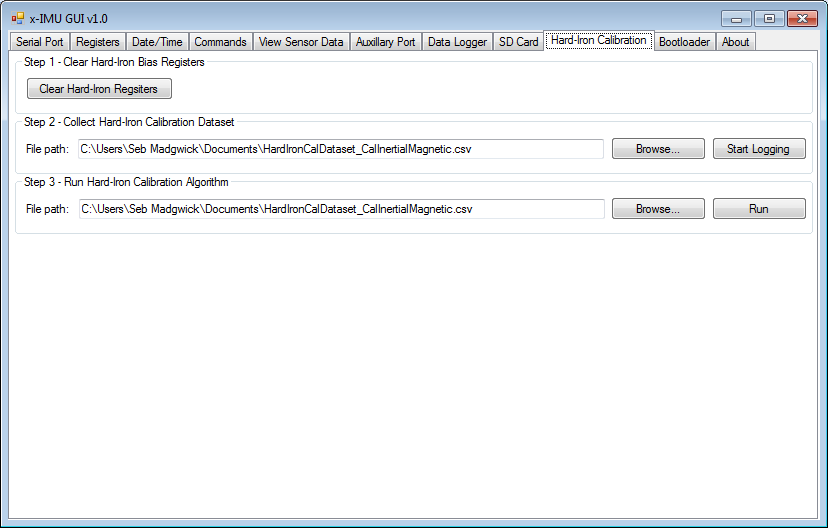
\includegraphics[width=0.8\textwidth]{graphics/GUI_tab_hard_iron_calibration.png}
		\caption{x-IMU GUI{} hard-iron calibration tab page}
	\label{fig:GUI_tab_hard_iron_calibration}
\end{figure}

The SD card socket will have different magnetic characteristics depending if an SD card is secured in the socket or not.  Each x-IMU is calibrated at the factory with a dummy SD card inserted to reduce the need for user calibration.

%- Calibrated sensor requires that the parameters of each sensor calibraiton model are defined.
%- IMU and AHRS algorithms require sensors to be calibrated.
%- For greatest accuracy, each x-IMU should be uniquly calibrated
%- Mechanical stress (e..g in box or fassened to chassis) and temperature affect sensor bahaviour and require differnt calribation parameters... for greatest accuracy user should calibrate each sensor while the x-IMU is in state of final applcaition
%- x-IMU supplied calibrated
%- The x-IMU can be fully calibrated by on-board algorithm access through user via comamnds and the x-IMU GUI without the need for specialist equitpment.
%
%%\sectionComingSoon{}

%%---------------------------------------------------------------------------------------------------
%\subsection{Gyroscope calibration}
%\label{sec:GyroscopeCalibration}
%
%\sectionComingSoon{}
%
%%------------------------------------------------
%\subsubsection{Gyroscope sensitivity calibration}
%\label{sec:GyroscopeSensitivityCalibration}
%
%\sectionComingSoon{}
%
%%------------------------------------------------
%\subsubsection{Gyroscope bias calibration}
%\label{sec:GyroscopeBiasCalibration}
%
%\sectionComingSoon{}
%
%%---------------------------------------------------------------------------------------------------
%\subsection{Accelerometer calibration}
%\label{sec:AccelerometerCalibration}
%
%\sectionComingSoon{}
%
%%---------------------------------------------------------------------------------------------------
%\subsection{Magnetometer calibration}
%\label{sec:MagnetometerCalibration}
%
%\sectionComingSoon{}
%
%%------------------------------------------------
%\subsubsection{Magnetometer bias and sensitivity calibration}
%\label{sec:MagnetometerBiasAndSensitivityCalibration}
%
%\sectionComingSoon{}
%
%%------------------------------------------------
%\subsubsection{Magnetometer hard-iron calibration}
%\label{sec:MagnetometerHardIronCalibration}
%
%\sectionComingSoon{}

%The sensors must be correctly calibrated for the IMU and AHRS algorithms to provide an accurate estimate of orientation.  The battery voltmeter must be correctly calibrated for the low battery voltage detection functionality to work properly.
%
%...save registers when done
%
%... For accurate calibration users should calibrate the x-IMU while it is in its intedned state...
%... all register settings... SD card connected or not...
%
%
%Each x-IMU is supplied pre-calibrated to provide an acceptable level of perfomrance for most user applcaitons.  All calibration parameters are defined in the registers ()
%
%
%%\subsection{When to re-calibrate}
%%\label{sec:WhenToReCalibrate}
%%
%%It is recommended that the user re-calibrated all sensors once the x-IMU is installed within its final application.  Doing so will ensure that any changes to sensor characteristics due to mechanical stresses, operating temperature range, mechanical stresses or magnetic environment, are accounted for by calibration.
%%
%%\paragraph{Changes to temperture:}
%%
%%\paragraph{Changes to mechancial stresses:} Mechcanical stresses to the x-IMU may cause changes to sensor characterstics.  The gyroscope bias is particaully sensitve to mechaicnal stresses.
%%
%%\paragraph{Changes to magnetic characterstics:}
%%
%%SD card.
%
%%------------------------------------------------
%\subsection{Gyroscope calibration}
%\label{sec:GyroscopeCalibration}
%
%
%The gyroscope calibration model used by the x-IMU and described in section \ref{sec:Gyroscope} requires that values for the sensitivities $s_{g_x}$, $s_{g_y}$ and $s_{g_z}$, biases at 25$^{\circ}$C $b_{g_x}$, $b_{g_y}$ and $b_{g_z}$ and bias temperature sensitivities $f_x$, $f_y$ and $f_z$ are defined within the gyroscope calibration registers (\ref{sec:GyroscopeXAxisSensitivity} to \ref{sec:GyroscopeZAxisBiasTemperatureSensitivity}).
%
%\paragraph{Gyroscope sensitivities}
%\label{sec:GyroscopeSensitivities}
%The sensitivities $s_{g_x}$, $s_{g_y}$ and $s_{g_z}$ are pre-calibrated by the gyroscope manufacturer.  The typical values quoted in the gyroscope datasheet are used by all x-IMUs and will provide sufficient accuracy for most user applications.  See the \gyroName{} datasheet for specific details on these parameters.
%
%\paragraph{Gyroscope biases}
%\label{sec:GyroscopeBiases}
%The gyroscope biases at 25$^{\circ}$C $b_{g_x}$, $b_{g_y}$ and $b_{g_z}$ and bias temperature sensitivities $f_x$, $f_y$ and $f_z$ vary between different x-IMUs and are uniquely calibrated for each unit using the on-board gyroscope bias calibration algorithm (\ref{sec:GyroscopeBiasCalibraitonAlgorithm}).  The gyroscope biases parameters are extrmely senstive to mechanical strain affecting the PCB.
%
%%---------------------------------------------------------------------------------------------------
%\subsubsection{Gyroscope bias calibration algorithm}
%\label{sec:GyroscopeBiasCalibraitonAlgorithm}
%
%The
%
%- x-IMU warms up while switched on and its operating temperature may depend of settings and usage.
%
%%---------------------------------------------------------------------------------------------------
%\subsection{Accelerometer calibration}
%\label{sec:AccelerometerCalibration}
%
%The accelerometer calibration model used by the x-IMU and described in section \ref{sec:Accelerometer} requires that values for the sensitivities $s_{a_x}$, $s_{a_y}$ and $s_{a_z}$ and biases $b_{a_x}$, $b_{a_y}$ and $b_{a_z}$ are defined within the accelerometer calibration registers (\ref{sec:AccelerometerXAxisSensitivity} to \ref{sec:AccelerometerZAxisBias}).
%
%\paragraph{Accelerometer sensitivities}
%\label{sec:AccelerometerSensitivities}
%
%
%
%%---------------------------------------------------------------------------------------------------
%\subsection{Magnetometer calibration}
%\label{sec:MagnetometerCalibration}
%
%...
%
%%---------------------------------------------------------------------------------------------------
%\subsubsection{Magnetometer calibration algorithm}
%\label{sec:MagnetometerCalibraitonAlgorithm}
%
%...
%
%%------------------------------------------------
%\subsubsection{Hard-iron calibration}
%\label{sec:MagnetometerHardIronCalibration}
%
%...

%=====================================================================================================
\section{IMU and AHRS algorithms}
\label{sec:IMUAndAHRSAlgorithms}

The x-IMU features an sensor fusion algorithm that use the on-board sensors to compute a measurement of orientation relative to the Earth.  The algorithm can operate in either IMU or AHRS mode.  IMU mode uses only the gyroscope and accelerometer.  In this mode, the head component of the measurement orientation will slowly drift over time.  However, magnetic distortions or interference will have no effect on the sensor as the magnetometer is not used.  IMU mode is of use in application that require only an accurate measurement of the pitch and roll components of an orientation or do not need an absolute measurement of heading.  AHRS mode uses all of the on-board sensors so that the measurement of orientation is free from drift.

The sensor fusion algorithm has a number of associated commands.  The Initialise command will cause the algorithm to reinitialise so that the proportional gain (Kp) governing how quickly the algorithm output converges to the accelerometer and magnetometer measurements, starts at a high value and is ramped down to the operating value.  The Tare command will save the current orientation so that all algorithm becomes relative to this datum.  A Tare operation is saved to non-volatile memory and so will remain in effect even if the device is reset.  A Clear Tare command will cancel this operation and clear the memory.

%- On-board algorithms provde oreitnation relative to Earth
%- Uses gyro, accel, mag
%- Oreintation data provided as quaternion in quaternion packet.  Data output rate set by register
%- API includes class methods for conversion to rotation matrix and Euler angles.
%- Oreintation viewed in GUI with 3D cuboid and Euler angles.
%
%- Algorithm update rate = 256 Hz regardless of data output rate
%- Algorithm performance is dependant on calibration.
%- Performance can be tuned by adjusting algorithm paramters.  See section \ref{sec:OptimisingAlgorithmPerformance} for more information.
%
%
%%---------------------------------------------------------------------------------------------------
%\subsection{Principle of operation}
%\label{sec:PrincipleOfOperation}
%
%- use gyroscope data to estimate oreintaiton.... however gyroscope measeutnts alone cannot work because of drift.
%- this drift is compensated for through meaurments of the Earth's gravitational and magentic feilds, provided by the accelermeter and magnetoemter respectivly.
%- accelerometer measures accelerations and the direction of gravity.... it is used to counter drift relative to the Earth's surface; i.e. the estimated pitch and roll.  As the acceleoemter also measures accelerations as well as gravitry,
%- magnetometer measures direction fo Earth's magentic feild... used to counter drift relative to the magnetic poles of the Earth; i.e. in the estimated heading.
%- the proportional gain governs how much influence
%
%\paragraph{IMU mode:}
%- The IMU algorithm uses only the gyroscope and acceleormeter and so will not compensate for drift in heading.  This is suitable for many applciations where only pitch and roll are required and/or it is possible to `reset' heading periodically.
%- The advantage of excluding the magnetoemter from the algorithm is: magnetic calbration unessary, local magnetic distortion have no effect; e.g. if x-IMU used within a magnetically noisey enviroment
%
%\paragraph{AHRS mode:}
%- The IMU algorithm uses only the gyroscope and acceleormeter and magnetoemer.  Free form drift in all axes.  As magnetoem
%
%
%%---------------------------------------------------------------------------------------------------
%\subsection{Algorithm parameters}
%\label{sec:AlgorithmParameters}
%
%%------------------------------------------------
%\subsubsection{Algorithm mode}
%\label{sec:AlgorithmMode}
%
%%------------------------------------------------
%\subsubsection{Algorithm gains}
%\label{sec:AlgorithmGains}
%
%%------------------------------------------------
%\subsubsection{Algorithm magnetic feild rejection}
%\label{sec:AlgorithmMagneticFeildRejection}
%
%%------------------------------------------------
%\subsubsection{Algorithm tare quaternion}
%\label{sec:AlgorithmTareQuaternion}
%
%
%%---------------------------------------------------------------------------------------------------
%\subsection{Algorithm operations}
%\label{sec:AlgorithmOperations}
%
%%------------------------------------------------
%\subsubsection{Algorithm initialise}
%\label{sec:AlgorithmInitialise}
%
%- init on reset
%
%%------------------------------------------------
%\subsubsection{Algorithm tare}
%\label{sec:AlgorithmTare}
%
%%------------------------------------------------
%\subsubsection{Algorithm clear tare}
%\label{sec:AlgorithmClearTare}
%
%%------------------------------------------------
%\subsubsection{Algorithm initialise then tare}
%\label{sec:AlgorithmInitialiseThenTare}
%
%%---------------------------------------------------------------------------------------------------
%\subsection{Optimising algorithm performance}
%\label{sec:OptimisingAlgorithmPerformance}

%The on-board sensor fusion algorithm uses the gyroscope, accelerometer and magnetometer to provide an optimal, real-time estimate of the devices' orientation relative to the Earth.  The IMU and AHRS algorithms require that the on-board sensors are properly calibrated (\ref{sec:Calibration}).  The estimated orientation is represented as a quaternion and is transmitted in the quaternion data packet \ref{sec:QuaternionData}.  The algorithm internal update rate is fixed at 256 Hz regardless of the quaternion data output rate (\ref{sec:QuaternionDataOutputRate}).
%
%
%%---------------------------------------------------------------------------------------------------
%\subsection{Algorithm modes}
%\label{sec:AlgorithmModes}
%
%The algorithm can run in either IMU (Inertial Measurement Unit) or AHRS (Attitude Heading Reference System) mode (\ref{sec:AlgorithmMode}).
%
%\paragraph{IMU mode}
%\label{sec:IMUMode}
%In IMU mode, only the gyroscope and accelerometer are used.  In this mode, the heading component of the estimated orientation will be subject to integral drift so that only the pitch and roll components may be trusted to be accurate.  The advantage using IMU mode is that magnetic measurements are completely ignored and so cannot corrupt the estimated orientation.  This is of use in applications that only require the pitch and roll components of a measured orientation; for example, camera stabilisation.
%
%\paragraph{AHRS mode}
%\label{sec:AHRSMode}
%In AHRS mode, the gyroscope, accelerometer and magnetometer are all used.  In this mode the estimated orientation is not subject to any integral drift.
%
%
%%---------------------------------------------------------------------------------------------------
%\subsection{Algorithm gains}
%\label{sec:AlgorithmGains}
%
%\paragraph{Proportional gain}
%\label{sec:ProportionalGain}
%The proportional feedback gain governs the rate at which the algorithm output converges to an orientation assumed by the accelerometer (in IMU mode) and magnetometer (in AHRS mode) measurements.  A large gain will mean that the estimated orientation will converge quickly and so will result in a 'shaky' orientation that is corrupted by linear accelerations and temporal magnetic distortions.  A low gain will mean that the estimated orientation 'trust the gyroscopes more' and result in a 'smooth' orientation; however, the algorithm will be less able to compensate for errors in the gyroscope measurements and calibration.  If a proportional gain of zero is used, then accelerometer and magnetometer measurements are completely ignored.
%
%\paragraph{Integral gain}
%\label{sec:IntegralGain}
%...
%
%%---------------------------------------------------------------------------------------------------
%\subsection{Algorithm operations}
%\label{sec:AlgorithmOperations}
%
%%------------------------------------------------
%\subsubsection{Reset algorithm}
%\label{sec:ResetAlgorithm}
%
%%------------------------------------------------
%\subsubsection{Tare}
%\label{sec:Tare}
%
%%------------------------------------------------
%\subsubsection{Clear tare}
%\label{sec:ClearTare}

%%---------------------------------------------------------------------------------------------------
%\subsection{Algorithm operations}
%\label{sec:AlgorithmOperations}
%
% OPTIMISING ALGORITHM PEROFRMANCE!!!


%=====================================================================================================
\section{Power management}
\label{sec:PowerManagement}

The x-IMU may be powered via \hyperref[sec:USB]{USB}, an \hyperref[sec:ExternalSupply]{external power supply} or a single cell lithium polymer (LiPo) \hyperref[sec:BatteryAndCharging]{battery} cell which will be \hyperref[sec:BatteryAndCharging]{charged} automatically while the x-IMU is connected to a \hyperref[sec:USB]{USB} port.

%---------------------------------------------------------------------------------------------------
\subsection{External supply}
\label{sec:ExternalSupply}

The x-IMU may be powered by a 3.5 to 6.3 V external supply via the \hyperref[sec:AuxiliaryPort]{auxiliary port}.  The supply should be connected to the \textit{GND} and \textit{EXT} pins of the \hyperref[sec:AuxiliaryPort]{auxiliary port}.  This power supply is only enabled while the \hyperref[sec:PowerSwitch]{power switch} is in the \textit{off} position.  In this situation, the \hyperref[sec:BatteryVoltmeter]{battery voltmeter} will measure the voltage of the external supply.

%---------------------------------------------------------------------------------------------------
\subsection{Battery and charging}
\label{sec:BatteryAndCharging}

The x-IMU has a standard connector for a 3.7 V single cell Lithium Polymer (LiPo) battery cell.  These batteries are widely available in range of capacities, for example \href{http://www.sparkfun.com/products/339}{1000 mAh} and \href{http://www.sparkfun.com/products/8483}{2000 mAh}.  The battery life is dependent on user settings and usage.  See the \hyperref[sec:TipsForMinimisingPowerConsumption]{tips on minimising power consumption} section.

The x-IMU has an on-board battery charger specially designed for LiPo battery cells.  The battery is charged automatically while the x-IMU is connected to a USB port.  The \hyperref[sec:ChargingLEDRed]{red charging LED} will remain lit while the battery is charging.  Charging stops automatically once complete.  The x-IMU may be used as normal while the battery is charging.  It is not necessary for the connected computer to have the USB drivers installed for charging, however the charging process will be faster if the drivers are installed.

%---------------------------------------------------------------------------------------------------
\subsection{Sleep mode}
\label{sec:SleepMode}

In sleep mode, the x-IMU remains powered but all on-board components are shutdown.  This allows the device to be powered down without removing power from essential components; for example, the \hyperref[sec:RealTimeClockAndCalendar]{real time clock and calendar}.  The \hyperref[sec:StatusLEDGreen]{green status LED} will blink once every 3 seconds to indicate that the device is in sleep mode.  Sleep mode is enabled through the sources listed below.  The x-IMU will reset upon wake up so that the same behaviour may be expected when the devices is powered on, reset or awakened.  The wake up sources are listed below.

\paragraph{Sleep mode enable sources:}
\label{sec:SleepModeEnableSources}

\begin{itemize}
	\item \hyperref[sec:CommandButton]{Command button} in sleep/wake mode
	\item \hyperref[sec:Sleep]{Sleep} command via \hyperref[sec:USB]{USB}, \hyperref[sec:Bluetooth]{Bluetooth} or \hyperref[sec:UART]{UART}
	\item \hyperref[sec:LowBatteryVoltageDetection]{Low battery voltage detection}
	\item \hyperref[sec:SleepTimer]{Sleep timer}
    \item \hyperref[sec:sleepWakeMode]{Sleep/wake mode}
\end{itemize}

\paragraph{Wake up sources}
\label{sec:WakeUpSources}

\begin{itemize}
	\item \hyperref[sec:CommandButton]{Command button} in sleep/wake mode
	\item \hyperref[sec:MotionTriggeredWakeUp]{Motion trigger wake up}
\end{itemize}

%---------------------------------------------------------------------------------------------------
\subsection{Low battery voltage detection}
\label{sec:LowBatteryVoltageDetection}

The calibrated \hyperref[sec:BatteryVoltmeter]{battery voltmeter} is used to trigger \hyperref[sec:SleepMode]{sleep mode} when the battery voltage falls below a specific level defined in the \textit{\hyperref[sec:BatteryShotdownVoltage]{battery shutdown voltage}} register.  This allows the x-IMU to execute critical tasks prior to power failure; for example closing the file on the \hyperref[sec:SDCard]{SD card} and notifying the user or host software with a \textit{\hyperref[sec:LowBattery]{low battery}} error.  By entering \hyperref[sec:SleepMode]{sleep mode} prior to power failure the x-IMU also ensures that the date and time of the \hyperref[sec:RealTimeClockAndCalendar]{real-time clock and calendar} are not lost.  The low battery voltage detection is disabled while \hyperref[sec:USB]{USB} is connected.

%---------------------------------------------------------------------------------------------------
\subsection{Sleep timer}
\label{sec:SleepTimer}

The sleep timer will trigger \hyperref[sec:SleepMode]{sleep mode} after the period of time defined in the \textit{\hyperref[sec:SleepTimerReg]{sleep timer}} register has elapsed.  The sleep timer countdown starts when the x-IMU starts up and may be reset by the sources listed below.  These sources enable the detection of motion, the user or the host software to prevent the x-IMU from entering \hyperref[sec:SleepMode]{sleep mode}.  The sleep timer is disabled by specifying a \textit{\hyperref[sec:SleepTimerReg]{sleep timer}} register value of 0 seconds.  The sleep timer is disabled while \hyperref[sec:USB]{USB} is connected.

\paragraph{Sleep timer reset sources}
\label{sec:SleepTimerResetSources}

\begin{itemize}
	\item \textit{\hyperref[sec:ResetSleepTimer]{reset sleep timer}} command
	\item \hyperref[sec:MotionTriggeredWakeUp]{Motion trigger wake up}
\end{itemize}

%---------------------------------------------------------------------------------------------------
\subsection{Motion triggered wake up}
\label{sec:MotionTriggeredWakeUp}

The motion trigger wake up is enabled via the \textit{\hyperref[sec:MotionTriggerWakeUpReg]{motion trigger wake up}} register and may be either \textit{disabled} or set to a \textit{low} or \textit{high} sensitivity.  Motion is detected using accelerometer.  If motion is detected while the x-IMU is in \hyperref[sec:SleepMode]{sleep mode} then the x-IMU will wake up.  While the x-IMU is not in \hyperref[sec:SleepMode]{sleep mode} the motion trigger wake up is used to reset the \hyperref[sec:SleepTimer]{sleep timer} and thus postpone sleep while motion persists.

For example, if the sleep timer is set to 20 seconds and there is motion is detected at least once every 20 seconds the motion trigger wake up will prevent the sleep timer from expiring and the x-IMU will not enter \hyperref[sec:SleepMode]{sleep mode}.  However, if no motion is detected for 20 seconds the x-IMU will enter \hyperref[sec:SleepMode]{sleep mode}.  If motion is then detected while in \hyperref[sec:SleepMode]{sleep mode}, the x-IMU will wake up.

%---------------------------------------------------------------------------------------------------
\subsection{Tips for minimising power consumption}
\label{sec:TipsForMinimisingPowerConsumption}

Battery powered applications require that power consumption is minimised in order to extend the battery life.  The x-IMU is designed to optimise power consumption according to user settings.  The user may therefore expect a considerable reduction in power consumption and extended battery life simply by using register settings appropriate to their application.

\paragraph{Tips}
\label{sec:Tips}

\begin{itemize}
	\item Set \hyperref[sec:BatteryAndThermometerDataOutputRate]{data output rates} of unused data to \textit{disabled}.
	\item Use the minimum \hyperref[sec:BatteryAndThermometerDataOutputRate]{data output rates} required by application.
	\item Set \hyperref[sec:AlgorithmMode]{algorithm mode} to \textit{disabled} if the \hyperref[sec:IMUAndAHRSAlgorithms]{IMU and AHRS algorithms} are not required.
	\item Disable \hyperref[sec:BluetoothPower]{Bluetooth power} if not Bluetooth is unused.
	\item Use the \hyperref[sec:SleepTimer]{sleep timer} and \hyperref[sec:MotionTriggeredWakeUp]{motion trigger wake up} to automatically enter \hyperref[sec:SleepMode]{sleep mode} during periods of inactivity.
\end{itemize}

%=====================================================================================================
\section{Auxiliary port}
\label{sec:AuxiliaryPort}

%\sectionComingSoon{}

The x-IMU features an auxiliary port that can be configured to one of many modes.  The auxiliary port connector is a $2\times6$, 2.54 mm pitch female header socket.  The socket pins include: ground, an external power input, 3.3 V power output, hard reset and 8 I/O channels.  The pins are annotated in Figure \ref{fig:auxiliaryPortPins} and summarised in table \ref{tab:auxiliaryPortPins}.

\begin{figure}[H]
	\centering
		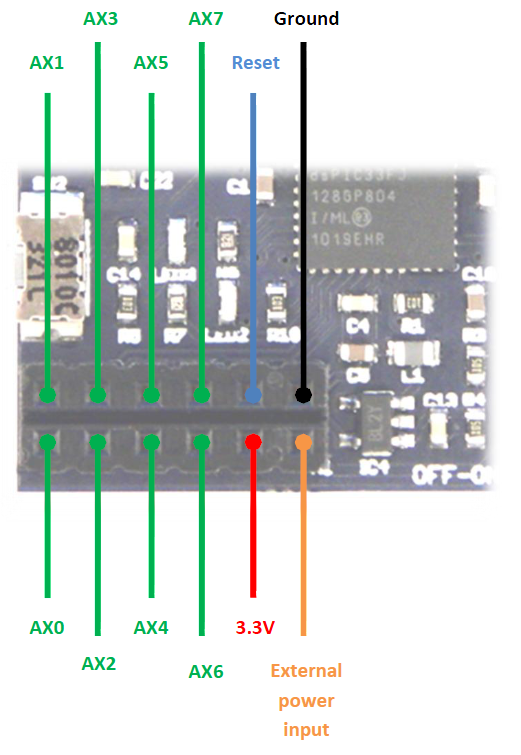
\includegraphics[width=0.5\textwidth]{graphics/auxiliaryPortPins.png}
		\caption{Auxiliary port pins}
	\label{fig:auxiliaryPortPins}
\end{figure}

\begin{table}[H]
	\centering
		\begin{tabular}{l l l}
		\hline
		Pin         &   Description             & Min/Max\\
		\hline
        GND         &   Common ground           & N/A\\
        EXT         &   External power input    & 3.5 V to 6.3 V\\
        RST         &   Hard reset (active low) & 0 V to 3.3 V\\
        3V3         &   3.3 V power output      & 100 mA\\
        AX0 to AX7  &   I/O channels            & 0 V to 3.3 V, 4 mA source/sink\\
		\hline
		\end{tabular}
		\caption{Auxiliary port pins}
	\label{tab:auxiliaryPortPins}
\end{table}

The mode of the auxiliary port is set by the \textit{\hyperref[sec:AuxiliaryPortMode]{auxiliary port mode}} register.  If the x-IMU receives a packet associated with a specific axillary port mode while the axillary port is not in that mode the x-IMU will respond with an \textit{\hyperref[sec:IncorrectAuxiliaryPortMode]{incorrect auxiliary port mode}} error.  For example, this will happen if the x-IMU receives a \textit{digital I/O packet} to change a digital output channel while the axillary port mode is \textit{disabled}.

\paragraph{Auxiliary port modes}
\begin{itemize}
  \item \hyperref[sec:Disabled]{Disabled}
  \item \hyperref[sec:DigitalIOMode]{Digital I/O}
  \item \hyperref[sec:AnalogueInput]{Analogue input}
  \item \hyperref[sec:PWMOutput]{PWM output}
  \item \hyperref[sec:ADXL345BusMode]{ADXL345 bus}
  \item \hyperref[sec:UART]{UART}
  \item \hyperref[sec:sleepWakeMode]{Sleep/wake mode}
\end{itemize}

\subsection{Disabled}
\label{sec:Disabled}

When \textit{disabled}, all auxiliary port channels are configured as high-impedance inputs.  The auxiliary port in \textit{disabled} when the x-IMU is in \hyperref[sec:SleepMode]{sleep mode}. Table \ref{tab:AuxiliaryPortPinAssignmentsWhenDisabled} summarises the auxiliary port pin assignments when disabled.

\begin{table}[H]
	\centering
		\begin{tabular}{l l l}
		\hline
		Pin       &   I/O     & Description\\
		\hline
        AX0       &   Input   & Unused\\
        AX1       &   Input   & Unused\\
        AX2       &   Input   & Unused\\
        AX3       &   Input   & Unused\\
        AX4       &   Input   & Unused\\
        AX5       &   Input   & Unused\\
        AX6       &   Input   & Unused\\
        AX7       &   Input   & Unused\\
		\hline
		\end{tabular}
		\caption{Auxiliary port pin assignments when disabled}
	\label{tab:AuxiliaryPortPinAssignmentsWhenDisabled}
\end{table}

\subsection{Digital I/O mode}
\label{sec:DigitalIOMode}

In \textit{digital I/O mode} each pin of the auxiliary port functions as either a digital input or output.  The direction of each pin is defined within the \textit{\hyperref[sec:DigitalIODirection]{digital I/O direction}} register.  Digital input data is provided in either the \textit{digital I/O data} packets received from the x-IMU.  The data output rate of these packets may be set to \textit{on change only}, 1 Hz, 2 Hz, 4 Hz, 8 Hz, 16 Hz, 32 Hz, 64 Hz, 128 Hz, 256 Hz or 512 Hz in the \textit{\hyperref[sec:DigitalIODataOutputRate]{digital I/O data output rate}} register.  Digital outputs are set by sending a \textit{digital I/O data} packet to the x-IMU.

\begin{table}[H]
	\centering
		\begin{tabular}{l l l}
		\hline
		Pin       &   I/O           & Description\\
		\hline
        AX0       &   Input/Output  & Digital I/O\\
        AX1       &   Input/Output  & Digital I/O\\
        AX2       &   Input/Output  & Digital I/O\\
        AX3       &   Input/Output  & Digital I/O\\
        AX4       &   Input/Output  & Digital I/O\\
        AX5       &   Input/Output  & Digital I/O\\
        AX6       &   Input/Output  & Digital I/O\\
        AX7       &   Input/Output  & Digital I/O\\
		\hline
		\end{tabular}
		\caption{Auxiliary port pin assignments in digital I/O mode}
	\label{tab:AuxiliaryPortPinAssignmentsInDigitalIOmode}
\end{table}

\subsection{Analogue input}
\label{sec:AnalogueInput}

In \textit{analogue input mode} all 8 pins of the auxiliary port function as analogue inputs.  Each analogue input channel sas a 12-bit resolution and a range of 0 V to 3.3 V.  The user may access analogue input data as either \textit{raw un-calibrated ADC results} or as \textit{calibrated units} by specifying the mode in the \textit{\hyperref[sec:AnalogueInputDataMode]{analogue input data mode}} register.  Analogue input data is provided in either the \textit{raw analogue input data} or \textit{calibrated analogue input data} packets.  The data output rate of these packets may be set to \textit{disabled}, 1 Hz, 2 Hz, 4 Hz, 8 Hz, 16 Hz, 32 Hz, 64 Hz, 128 Hz, 256 Hz or 512 Hz in the \textit{\hyperref[sec:AnalogueInputDataOutputRate]{analogue input data output rate}} register.

\paragraph{Raw ADC data:}
In raw data mode the analogue input data is the ADC integer value between 0 and 4096 corresponding to a voltage between 0 V and 3.3 V.  This data is provided in the \textit{raw analogue input data} packets.

\paragraph{Calibrated data:}
In calibrated data mode the analogue data is the calibrated measurement in Volts.  This data is provided in the \textit{calibrate analogue data} packets.  The calibrated measurement $a_n$ is calculated from the raw ADC measurements $\tilde{v}$ according to a sensitivity $s_{a_n}$ and bias $b_{a_n}$ as described by equation \eqref{analogueInputCal}.  Parameters $s_{a_n}$ and $b_{a_n}$ are defined in the analogue input \textit{\hyperref[sec:AnalogueInputSensitivity]{sensitivity}} and \textit{\hyperref[sec:AnalogueInputBias]{bias}} registers.

\begin{equation}
	a_n = \frac{1}{s_{a_n}} ( \tilde{a_n} - b_{a_n} )
	\label{analogueInputCal}
\end{equation}

\begin{table}[H]
	\centering
		\begin{tabular}{l  l l}
		\hline
		Pin       &   I/O     & Description\\
		\hline
        AX0       &   Input   & Analogue input channel AX0\\
        AX1       &   Input   & Analogue input channel AX1\\
        AX2       &   Input   & Analogue input channel AX2\\
        AX3       &   Input   & Analogue input channel AX3\\
        AX4       &   Input   & Analogue input channel AX4\\
        AX5       &   Input   & Analogue input channel AX5\\
        AX6       &   Input   & Analogue input channel AX6\\
        AX7       &   Input   & Analogue input channel AX7\\
		\hline
		\end{tabular}
		\caption{Auxiliary port pin assignments for analogue input mode}
	\label{tab:AuxPortPinAsignForAnalogueInputMode}
\end{table}

\subsection{PWM output mode}
\label{sec:PWMOutput}

In \textit{PWM output mode} four pins of the auxiliary port function as digital PWM outputs.  Unused pins are configured as high-impedance inputs.  The PWM frequency may be set from 3 Hz to 65,535 Hz in the \textit{\hyperref[sec:PWMFrequency]{PWM frequency}} register.  The duty cycle of each of the four PWM output channels are set by sending a \textit{PWM data} packet to the x-IMU.  The x-IMU echo back the packet as confirmation after the duty cycles have been set.

\begin{table}[H]
	\centering
		\begin{tabular}{l  l l}
		\hline
		Pin       &   I/O         & Description\\
		\hline
        AX0       &   Output    & PWM output channel AX0\\
        AX1       &   Input     & Unused\\
        AX2       &   Output    & PWM output channel AX2\\
        AX3       &   Input     & Unused\\
        AX4       &   Output    & PWM output channel AX4\\
        AX5       &   Input     & Unused\\
        AX6       &   Output    & PWM output channel AX6\\
        AX7       &   Input     & Unused\\
		\hline
		\end{tabular}
		\caption{Auxiliary port pin assignments for PWM output mode}
	\label{tab:AuxPortPinAsignForPWMoutputMode}
\end{table}

\subsection{ADXL345 bus mode}
\label{sec:ADXL345BusMode}

\sectionComingSoon{}

%- sensors need to init, this only happen when auxilary port mode changed or device start up... so if plug in sensor while x-IMU already in mdoe qnd running, the sensor will noot have been initilised and will not provde data.

\begin{table}[H]
	\centering
		\begin{tabular}{l  l l}
		\hline
		Pin       &   I/O         & Description\\
		\hline
        AX0       &   Output    & ADXL345 A SPI CS\\
        AX1       &   Input     & SPI CLK\\
        AX2       &   Output    & ADXL345 B SPI CS\\
        AX3       &   Input     & SPI DIN\\
        AX4       &   Output    & ADXL345 C SPI CS\\
        AX5       &   Input     & SPI DOUT\\
        AX6       &   Output    & ADXL345 D SPI CS\\
        AX7       &   Input     & Power enable\\
		\hline
		\end{tabular}
		\caption{Auxiliary port pin assignments for ADXL345 bus mode}
	\label{tab:AuxPortPinAsignForADXL345busMode}
\end{table}

\subsection{UART mode}
\label{sec:UART}

In \textit{UART mode} four pins of the auxiliary port function as a configurable UART with hardware flow control.  The \textit{\hyperref[sec:BluetoothPower]{Bluetooth power}} will automatically be disabled when \textit{UART mode} is enabled.  Commination via the auxiliary port UART is identical to that via the virtual serial ports enabled by the Bluetooth or USB connection.  The UART baud rate may be set to 2400, 4800, 7200, 9600, 14400, 19200, 38400, 57600, 115200, 230400, 460800 or 921600 baud in the \textit{\hyperref[sec:UARTBaudRate]{UART baud rate}} register.  The UART hardware flow control can be enabled or disabled in the \textit{\hyperref[sec:UARTHardwareFlowControl]{UART hardware flow control}} register.

\begin{table}[H]
	\centering
		\begin{tabular}{l  l l}
		\hline
		Pin       &   I/O         & Description\\
		\hline
        AX0       &   Output    & RX\\
        AX1       &   Input     & Unused\\
        AX2       &   Output    & TX\\
        AX3       &   Input     & Unused\\
        AX4       &   Output    & CTS\\
        AX5       &   Input     & Unused\\
        AX6       &   Output    & RTS\\
        AX7       &   Input     & Unused\\
		\hline
		\end{tabular}
		\caption{Auxiliary port pin assignments for UART mode}
	\label{tab:AuxPortPinAsignForUARTmode}
\end{table}

\subsubsection{UART bandwidth}
\label{sec:UARTBandwidth}

It is possible for the user to define \hyperref[sec:BatteryAndThermometerDataOutputRate]{data output rates} so that the amount of data being generated by the x-IMU exceeds the bandwidth of a communication channel.  If the UART bandwidth is exceed, the UART transmit buffer will overrun and some data will be lost.  When this happens a \textit{\hyperref[sec:UARTTransmitBufferOverrun]{UART transmit buffer overrun}} error will be generated.  As this error is sent immediately after the buffer has overrun, the error will be successfully transmitted.  This error can be avoided by reducing the \hyperref[sec:BatteryAndThermometerDataOutputRate]{data output rates} or increasing the \textit{\hyperref[sec:UARTBaudRate]{UART baud rate}} register.

All data sent to the x-IMU via UART is buffered in the UART receive buffer before being processed.  The time required to process the received data is dependent on the data.  If data is sent to the x-IMU via UART at a rate at a rate greater than it can be processed then the receive buffer will overflow and some data will be lost.  When this happens a \textit{\hyperref[sec:UARTReceiveBufferOverrun]{UART receive buffer overrun}} error will be generated.


\subsection{Sleep/wake mode}
\label{sec:sleepWakeMode}

In \textit{Sleep/wake mode} three pins of the auxiliary port function as an interface to control the sleep/wake state of the x-IMU remotely.  This may be useful in logging applications where access to the command button.  Separate inputs are assigned for sleep and wake signals to prevent accidental double triggering reverting an intended action.  An output signal indicates the sleep state of the x-IMU and can be used to drive an LED.

\begin{table}[H]
	\centering
		\begin{tabular}{l  l l}
		\hline
		Pin       &   I/O         & Description\\
		\hline
        AX0       &   Output    & Sleep (active low, with internal pull-up)\\
        AX1       &   Input     & Unused\\
        AX2       &   Output    & Wake (active low, with internal pull-up)\\
        AX3       &   Input     & Unused\\
        AX4       &   Output    & Sleep state (wake = driven low, sleep = pull-up)\\
        AX5       &   Input     & Unused\\
        AX6       &   Output    & Unused\\
        AX7       &   Input     & Unused\\
		\hline
		\end{tabular}
		\caption{Auxiliary port pin assignments for Sleep/Wake mode}
	\label{tab:AuxPortPinAsignForSLeepWakemode}
\end{table}

%=====================================================================================================
% Communication protocol
%=====================================================================================================
\section{Communication protocol}
\label{sec:CommunicationProtocol}

Documentation for the communication protocol used to interface to the x-IMU via serial is not provided.  However, an example generic C++ library is available on the x-IMU webpage and the \hyperref[sec:xIMUAPI]{x-IMU API} source code written in C\# provides a compressive library for all functionally of the x-IMU.

%%---------------------------------------------------------------------------------------------------
%\subsection{Packet encoding}
%\label{sec:PacketEncoding}
%
%This section is incomplete.  Please contact \verb=www.x-io.co.uk= for the document to be updated.
%
%%---------------------------------------------------------------------------------------------------
%\subsection{Checksum}
%\label{sec:Checksum}
%
%This section is incomplete.  Please contact \verb=www.x-io.co.uk= for the document to be updated.
%
%%---------------------------------------------------------------------------------------------------
%\subsection{Packet types}
%\label{sec:PacketTypes}
%
%%------------------------------------------------
%\subsubsection{Error message}
%\label{sec:ErrorMessage}
%
%This section is incomplete.  Please contact \verb=www.x-io.co.uk= for the document to be updated.
%
%%------------------------------------------------
%\subsubsection{Command message}
%\label{sec:CommandMessage}
%
%This section is incomplete.  Please contact \verb=www.x-io.co.uk= for the document to be updated.
%
%%------------------------------------------------
%\subsubsection{Read register}
%\label{sec:ReadRegister}
%
%This section is incomplete.  Please contact \verb=www.x-io.co.uk= for the document to be updated.
%
%%------------------------------------------------
%\subsubsection{Write register}
%\label{sec:WriteRegister}
%
%This section is incomplete.  Please contact \verb=www.x-io.co.uk= for the document to be updated.
%
%%------------------------------------------------
%\subsubsection{Raw battery and thermometer data}
%\label{sec:RawBatteryAndThermometerData}
%
%This section is incomplete.  Please contact \verb=www.x-io.co.uk= for the document to be updated.
%
%%------------------------------------------------
%\subsubsection{Calibrated battery and thermometer data}
%\label{sec:CalibratedBatteryAndThermometerData}
%
%This section is incomplete.  Please contact \verb=www.x-io.co.uk= for the document to be updated.
%
%%------------------------------------------------
%\subsubsection{Raw inertial and magnetic data}
%\label{sec:RawInertialAndMagneticData}
%
%This section is incomplete.  Please contact \verb=www.x-io.co.uk= for the document to be updated.
%
%%------------------------------------------------
%\subsubsection{Calibrated inertial and magnetic data}
%\label{sec:CalibratedInertialAndMagneticData}
%
%This section is incomplete.  Please contact \verb=www.x-io.co.uk= for the document to be updated.
%
%%------------------------------------------------
%\subsubsection{Quaternion data}
%\label{sec:QuaternionData}
%
%This section is incomplete.  Please contact \verb=www.x-io.co.uk= for the document to be updated.

%=====================================================================================================
% Commands
%=====================================================================================================
\section{Commands}
\label{sec:Commands}

Commands are executed by either sending a \textit{command} packet to the x-IMU \hyperref[sec:USB]{USB} or \hyperref[sec:Bluetooth]{Bluetooth} or by pressing the \hyperref[sec:CommandButton]{command button} which may be configured to execute a specific command.  Commands are sent using the x-IMU GUI{} via the \textit{\hyperref[sec:TabPageCommands]{commands}} tab page.  Once a command has been executed, the x-IMU will echo the \textit{command} packet back to the host as confirmation.  As all communication from the x-IMU to the host computer is logged to the \hyperref[sec:SDCard]{SD card}, all command confirmations will be logged on the \hyperref[sec:SDCard]{SD card}.  If a \textit{command} packet is sent containing an invalid command code the x-IMU will respond with an \textit{\hyperref[sec:InvalidCommand]{invalid command}} error.

Sending a \textit{command} packet to the x-IMU will cause the x-IMU to momentarily pause sensor sampling and processing while the received data is processed.  This may cause discrepancies in the otherwise fixed data output rates.

% And data will not be processed while packet being dealt with.  This may cause receive buffer overrun errors.

%---------------------------------------------------------------------------------------------------
\subsection{Individual commands}
\label{sec:IndividualCommands}

%------------------------------------------------
\subsubsection{Null command}
\label{sec:NullCommand}

\begin{tabular*}{1.0\textwidth}{lp{0.815\textwidth} l}
	\textit{Command code:}	& \verb=0x0000=\\
	\textit{Description:}	& A \textit{null command} is a valid command code but will result in no action.  As all commands sent to the x-IMU are echoed back to the sender, a null command may be used by the host software to confirm communication with the x-IMU.
\end{tabular*}

%------------------------------------------------
\subsubsection{Factory reset}
\label{sec:FactoryReset}

\begin{tabular*}{1.0\textwidth}{lp{0.815\textwidth} l}
	\textit{Command code:}	& \verb=0x0001=\\
	\textit{Description:}	& A \textit{factory reset} command code is used to reset the x-IMU to its original state prior to factory calibration so that all registers return to their default values.  The user must press the \hyperref[sec:CommandButton]{command button} within 3 seconds of sending a \textit{factory reset} command in order to confirm the request else the x-IMU will respond with a \textit{\hyperref[sec:FactoryResetFailed]{factory reset failed}} error.  The x-IMU requires several seconds to reconfigure on-board components during the execution of a factory reset.
\end{tabular*}

%------------------------------------------------
\subsubsection{Reset}
\label{sec:Reset}

\begin{tabular*}{1.0\textwidth}{lp{0.815\textwidth} l}
	\textit{Command code:}	& \verb=0x0002=\\
	\textit{Description:}	& A \textit{reset} command causes a software reset of the x-IMU.  The x-IMU will close any open files on the SD card before reset, in this way the reset command may be of use to users wishing to break up a logging session into multiple files.  The reset command is used to put the x-IMU into bootloader mode in order to upload new firmware.  A \textit{reset} command is sent by the x-IMU to the host computer as confirmation of reset, power on and wake up.
\end{tabular*}

%------------------------------------------------
\subsubsection{Sleep}
\label{sec:Sleep}

\begin{tabular*}{1.0\textwidth}{lp{0.815\textwidth} l}
	\textit{Command code:}	& \verb=0x0003=\\
	\textit{Description:}	& A \textit{sleep} command will put the device into \hyperref[sec:SleepMode]{sleep mode}.  The x-IMU will close any open files on the \hyperref[sec:SDCard]{SD card} before entering \hyperref[sec:SleepMode]{sleep mode}.  The x-IMU may be taken out of \hyperref[sec:SleepMode]{sleep mode} by using the \hyperref[sec:CommandButton]{command button} configured in \textit{sleep/wake} mode or using the \hyperref[sec:MotionTriggeredWakeUp]{motion triggered wake up} functionality.
\end{tabular*}

%------------------------------------------------
\subsubsection{Reset sleep timer}
\label{sec:ResetSleepTimer}

\begin{tabular*}{1.0\textwidth}{lp{0.815\textwidth} l}
	\textit{Command code:}	& \verb=0x0004=\\
	\textit{Description:}	& The \textit{reset sleep timer} command will reset the \hyperref[sec:SleepTimer]{sleep timer} countdown and so postpone sleep.  An example usage of this command is to create behaviour where the x-IMU will automatically enter \hyperref[sec:SleepMode]{sleep mode} when communication with the host software ends or connection is lost.
\end{tabular*}

%------------------------------------------------
\subsubsection{Sample gyroscope axis at 200 dps}
\label{sec:SampleGyroscopeAxisAtPm200CircS}

\begin{tabular*}{1.0\textwidth}{lp{0.815\textwidth} l}
	\textit{Command code:}	& \verb=0x0005=\\
	\textit{Description:}	& The \textit{sample gyroscope axis at 200 dps} command is used to calibrate the gyroscope sensitivity parameters.  This command should be sent while the x-IMU rotating at either $+200^\circ$/s or $-200^\circ$/s around either its \textit{x}, \textit{y} or \textit{z} axis.  The x-IMU will automatically detect the axis and direction of rotation.  The mean gyroscope output will then be measured over approximately 8 seconds before being stored to the \hyperref[sec:GyroscopeSampledXAxisAtp200Dps]{corresponding register}.  A \textit{\hyperref[sec:CalculateGyroscopeSensitivity]{calculate gyroscope sensitivity}} command will then be executed.  The execution of the \textit{sample gyroscope axis at 200 dps} command will be aborted if a gyroscope axis is detected as not being at approximately $\pm200^\circ$/s and a \textit{\hyperref[sec:GyroscopeAxisNotAt200Dps]{gyroscope axis not at 200 dps}} error will be generated.  See the \hyperref[sec:GyroscopeSensitivityCalibration]{gyroscope sensitivity calibration} section for more information.
\end{tabular*}

%------------------------------------------------
\subsubsection{Calculate gyroscope sensitivity}
\label{sec:CalculateGyroscopeSensitivity}

\begin{tabular*}{1.0\textwidth}{lp{0.815\textwidth} l}
	\textit{Command code:}	& \verb=0x0006=\\
	\textit{Description:}	& The \textit{calculate gyroscope sensitivity} command is used to execute the on-board gyroscope sensitivity calibration algorithm.  The algorithm uses the \hyperref[sec:GyroscopeSampledXAxisAtp200Dps]{sampled gyroscope bias} register values previously obtained by the \textit{\hyperref[sec:SampleGyroscopeAxisAtPm200CircS]{sample gyroscope axis at 200 dps}} command to update the \hyperref[sec:GyroscopeXAxisSensitivity]{gyroscope sensitivity parameters registers}.  See the \hyperref[sec:GyroscopeSensitivityCalibration]{gyroscope sensitivity calibration} section for more information.
\end{tabular*}

%------------------------------------------------
\subsubsection{Sample gyroscope bias at temperature 1}
\label{sec:SampleGyroscopeBiasAtTemperature1}

\begin{tabular*}{1.0\textwidth}{lp{0.815\textwidth} l}
	\textit{Command code:}	& \verb=0x0007=\\
	\textit{Description:}	& The \textit{sample gyroscope bias at temperature 1} command is used to calibrate the gyroscope bias parameters.  This command should be sent while the x-IMU is stationary and at the lowest temperature the device is required to operate at.  The x-IMU will measure the mean temperature and gyroscope output over approximately  16 seconds, store the results to the \hyperref[sec:GyroscopeSample1Temperature]{sampled temperature 1} registers and then trigger a \textit{\hyperref[sec:CalculateGyroscopeBiasParameters]{calculate gyroscope bias parameters}} command.  The execution of the \textit{sample gyroscope bias at temperature 1} command will be aborted if the gyroscope is detected as not being stationary and a \textit{\hyperref[sec:GyroscopeNotStationary]{gyroscope not stationary}} error will be generated.  See the \hyperref[sec:GyroscopeBiasCalibration]{gyroscope bias calibration} section for more information.
\end{tabular*}

%------------------------------------------------
\subsubsection{Sample gyroscope bias at temperature 2}
\label{sec:SampleGyroscopeBiasAtTemperature2}

\begin{tabular*}{1.0\textwidth}{lp{0.815\textwidth} l}
	\textit{Command code:}	& \verb=0x0008=\\
	\textit{Description:}	& The \textit{sample gyroscope bias at temperature 2} command is used to calibrate the gyroscope bias parameters.  This command should be sent while the x-IMU is stationary and at the lowest temperature the device is required to operate at.  The x-IMU will measure the mean temperature and gyroscope output over approximately  16 seconds, store the results to the \hyperref[sec:GyroscopeSample2Temperature]{sampled temperature 2} registers and then trigger a \textit{\hyperref[sec:CalculateGyroscopeBiasParameters]{calculate gyroscope bias parameters}} command.  The execution of the \textit{sample gyroscope bias at temperature 2} command will be aborted if the gyroscope is detected as not being stationary and a \textit{\hyperref[sec:GyroscopeNotStationary]{gyroscope not stationary}} error will be generated.  See the \hyperref[sec:GyroscopeBiasCalibration]{gyroscope bias calibration} section for more information.
\end{tabular*}

%------------------------------------------------
\subsubsection{Calculate gyroscope bias parameters}
\label{sec:CalculateGyroscopeBiasParameters}

\begin{tabular*}{1.0\textwidth}{lp{0.815\textwidth} l}
	\textit{Command code:}	& \verb=0x0009=\\
	\textit{Description:}	& The \textit{calculate gyroscope bias parameters} command is used to execute the on-board gyroscope bias calibration algorithm.  The algorithm uses the \hyperref[sec:GyroscopeSample1Temperature]{sampled gyroscope bias} register values previously sampled by the \textit{\hyperref[sec:SampleGyroscopeBiasAtTemperature1]{sample gyroscope bias at temperature 1}} and \textit{\hyperref[sec:SampleGyroscopeBiasAtTemperature2]{sample gyroscope bias at temperature 2}} commands to calculate the gyroscope bias parameters and update the \hyperref[sec:GyroscopeXAxisBias]{gyroscope bias parameters} registers.  See the \hyperref[sec:GyroscopeBiasCalibration]{gyroscope bias calibration} section for more information.
\end{tabular*}

%------------------------------------------------
\subsubsection{Sample accelerometer axis at 1 g}
\label{sec:SampleAccelerometerAxisAt1G}

\begin{tabular*}{1.0\textwidth}{lp{0.815\textwidth} l}
	\textit{Command code:}	& \verb=0x000A=\\
	\textit{Description:}	& The \textit{sample accelerometer axis at 1 g} command is used to calibrate the accelerometer bias and sensitivity parameters.  This command should be sent while the x-IMU stationary and orientated with either its \textit{x}, \textit{y} or \textit{z} axis at either $+1$ g or $-1$ g.  The x-IMU will automatically detect the axis and direction of gravity.  The mean accelerometer output will then be measured over approximately 8 seconds before being stored to the \hyperref[sec:AccelerometerSampledXAxisAtp1G]{sampled accelerometer axis} registers.  A \textit{\hyperref[sec:CalculateAccelerometerBiasAndSensitivity]{calculate accelerometer bias and sensitivity}} command will then be executed.  The execution of the \textit{sample accelerometer axis at 1 g} command will be aborted if a accelerometer axis is detected as not being at approximately $\pm1$ g and a \textit{\hyperref[sec:AccelerometerAxisNotAt1g]{accelerometer axis not at 1 g}} error will be generated.  See the \hyperref[sec:AccelerometerCalibration]{accelerometer calibration} section for more information.
\end{tabular*}

%------------------------------------------------
\subsubsection{Calculate accelerometer bias and sensitivity}
\label{sec:CalculateAccelerometerBiasAndSensitivity}

\begin{tabular*}{1.0\textwidth}{lp{0.815\textwidth} l}
	\textit{Command code:}	& \verb=0x000B=\\
	\textit{Description:}	& The \textit{calculate accelerometer bias and sensitivity} command is used to execute the on-board accelerometer bias and sensitivity calibration algorithm.  The algorithm uses the \hyperref[sec:AccelerometerSampledXAxisAtp1G]{sampled accelerometer axes} register values previously obtained by the \textit{\hyperref[sec:SampleAccelerometerAxisAt1G]{sample accelerometer axis at 1 g}} command to calculate the accelerometer bias and sensitivity and update the \hyperref[sec:AccelerometerXAxisSensitivity]{accelerometer calibration parameters} registers.  See the \hyperref[sec:AccelerometerCalibration]{accelerometer calibration} section for more information.
\end{tabular*}

%------------------------------------------------
\subsubsection{Measure magnetometer bias and sensitivity}
\label{sec:MeasureMagnetometerBiasAndSensitivity}

\begin{tabular*}{1.0\textwidth}{lp{0.815\textwidth} l}
	\textit{Command code:}	& \verb=0x000C=\\
	\textit{Description:}	& The \textit{measure magnetometer bias and sensitivity} command is used to run an on-board magnetometer calibration algorithm.  The x-IMU uses the magnetometer's internal field generator to measure the mean magnetometer bias and sensitivity over approximately 16 seconds independent of external magnetic interference.  The magnetometer \hyperref[sec:MagnetometerXAxisSensitivity]{sensitivity} and \hyperref[sec:MagnetometerXAxisBias]{bias} registers and then automatically updated.  This command should be used each time the \hyperref[sec:MagnetometerFullScale]{magnetometer full-scale range} is changed.  The execution of this command will be aborted if a magnetometer axis saturates and a \textit{\hyperref[sec:MagnetometerSaturation]{magnetometer saturation}} error will be generated.  See the \hyperref[sec:MagnetometerCalibration]{magnetometer calibration} section for more information.
\end{tabular*}

%------------------------------------------------
\subsubsection{Algorithm initialise}
\label{sec:AlgorithmInitialise}

\begin{tabular*}{1.0\textwidth}{lp{0.815\textwidth} l}
	\textit{Command code:}	& \verb=0x000D=\\
	\textit{Description:}	& The \textit{algorithm initialise} command will re-start the algorithm from initial conditions.  This command can be used to 'force' the algorithm to converge to steady state conditions if previous distortions to magnetic or other extreme sensor measurements have left the IMU or AHRS algorithm output at an erroneous orientation.  See the \hyperref[sec:IMUAndAHRSAlgorithms]{IMU and AHRS algorithms} section for more information.
\end{tabular*}

%------------------------------------------------
\subsubsection{Algorithm tare}
\label{sec:AlgorithmTare}

\begin{tabular*}{1.0\textwidth}{lp{0.815\textwidth} l}
	\textit{Command code:}	& \verb=0x000E=\\
	\textit{Description:}	& The \textit{algorithm tare} command is used to set the algorithm datum orientation and store the reference quaternion to the \textit{\hyperref[sec:TareQuaternionElement0]{tare quaternion}} registers.  These registers may be then be cleared using the \textit{\hyperref[sec:AlgorithmClearTare]{algorithm clear tare}} command.  See the \hyperref[sec:IMUAndAHRSAlgorithms]{IMU and AHRS algorithms} section for more information.
\end{tabular*}

%------------------------------------------------
\subsubsection{Algorithm clear tare}
\label{sec:AlgorithmClearTare}

\begin{tabular*}{1.0\textwidth}{lp{0.815\textwidth} l}
	\textit{Command code:}	& \verb=0x000F=\\
	\textit{Description:}	& The \textit{algorithm clear tare} command is used to clear the \textit{\hyperref[sec:TareQuaternionElement0]{tare quaternion}} registers and return the datum orientation to alignment with the Earth coordinate frame.  See the \hyperref[sec:IMUAndAHRSAlgorithms]{IMU and AHRS algorithms} section for more information.
\end{tabular*}

%------------------------------------------------
\subsubsection{Algorithm initialise then tare}
\label{sec:AlgorithmInitialiseThenTare}

\begin{tabular*}{1.0\textwidth}{lp{0.815\textwidth} l}
	\textit{Command code:}	& \verb=0x0010=\\
	\textit{Description:}	& The \textit{algorithm initialise then tare} command will perform an \textit{\hyperref[sec:AlgorithmInitialise]{algorithm initialise}} and then \textit{\hyperref[sec:AlgorithmTare]{algorithm tare}}  once the initialisation is complete.  See the \hyperref[sec:IMUAndAHRSAlgorithms]{IMU and AHRS algorithms} section for more information.
\end{tabular*}

%=====================================================================================================
% Errors
%=====================================================================================================
\section{Errors}
\label{sec:Errors}

Error are sent by the x-IMU to warn the user or host software of any internal errors that have occurred.  Error data is sent in \textit{error} packets.  The \hyperref[sec:xIMUGUI]{x-IMU GUI} will display these errors in message boxes for user acknowledgment.  As all data packets generated by the x-IMU are logged to the \hyperref[sec:SDCard]{SD card}, the \hyperref[sec:SDCard]{SD card} will contain a record off errors.

%---------------------------------------------------------------------------------------------------
\subsection{Individual errors}
\label{sec:IndividualErrorMessages}

%------------------------------------------------
\subsubsection{No error}
\label{sec:NoError}

\begin{tabular*}{1.0\textwidth}{lp{0.845\textwidth} l}
	\textit{Error code:}	& \verb=0x0000=\\
	\textit{Description:}	& No error.  This error code is used within internal processes and will never appear to the user.
\end{tabular*}

%------------------------------------------------
\subsubsection{Factory reset failed}
\label{sec:FactoryResetFailed}

\begin{tabular*}{1.0\textwidth}{lp{0.845\textwidth} l}
	\textit{Error code:}	& \verb=0x0001=\\
	\textit{Description:}	& A \textit{factory reset failed} error is sent if the user fails to press the \hyperref[sec:CommandButton]{command button} within 3 seconds of sending a \textit{\hyperref[sec:FactoryReset]{factory reset}} command and the execution of the command was aborted.
\end{tabular*}

%------------------------------------------------
\subsubsection{Low battery}
\label{sec:LowBattery}

\begin{tabular*}{1.0\textwidth}{lp{0.845\textwidth} l}
	\textit{Error code:}	& \verb=0x0002=\\
	\textit{Description:}	& A \textit{low battery} error is sent when the low \hyperref[sec:LowBatteryVoltageDetection]{battery voltage detection} detects that the battery voltage has fallen below the specific level defined in the \textit{\hyperref[sec:BatteryShotdownVoltage]{battery shutdown voltage}} register.  This message is sent immediately before the x-IMU enters \hyperref[sec:SleepMode]{sleep mode}.  See the \hyperref[sec:LowBatteryVoltageDetection]{low battery voltage detection} section for more information.
\end{tabular*}

%------------------------------------------------
\subsubsection{USB receive buffer overrun}
\label{sec:USBReceiveBufferOverrun}

\begin{tabular*}{1.0\textwidth}{lp{0.845\textwidth} l}
	\textit{Error code:}	& \verb=0x0003=\\
	\textit{Description:}	& A \textit{USB receive buffer over} error will be sent if the \hyperref[sec:USB]{USB} receive buffer overruns and data to be received was lost.  This occurs when data is transmitted to the x-IMU at a rate greater than the rate it can be processed.  Consider reducing the rate at which data is sent to the x-IMU if this error occurs repeatedly.  See the \hyperref[sec:USBBandwidth]{USB bandwidth} section for more information.
\end{tabular*}

%------------------------------------------------
\subsubsection{USB transmit buffer overrun}
\label{sec:USBTransmitBufferOverrun}

\begin{tabular*}{1.0\textwidth}{lp{0.845\textwidth} l}
	\textit{Error code:}	& \verb=0x0004=\\
	\textit{Description:}	& A \textit{USB transmit buffer overrun} error will be sent if the USB transmit buffer overruns and data due to be transmitted was lost.  This will occur when the communication channel bandwidth is unable to cope with the amount of data being transmitted.  Consider using lower data output rates if this error occurs repeatedly.  This error may be ignored in applications where USB data is not essential and the SD card is the intended data output.  In such applications, the user need only be concerned with \textit{\hyperref[sec:SDCardWriteBufferOverrun]{SD card write buffer overrun}} errors.  The x-IMU will attempt to transmit data via \hyperref[sec:USB]{USB} while the \hyperref[sec:USB]{USB} is detected as connected, if the \hyperref[sec:USB]{USB} is connect but the associated serial port not open then the \hyperref[sec:USB]{USB} transmit buffer will continue to overrun until the port is opened or the \hyperref[sec:USB]{USB} disconnected.  See the \hyperref[sec:USBBandwidth]{USB bandwidth} section for more information.
\end{tabular*}

%------------------------------------------------
\subsubsection{Bluetooth receive buffer overrun}
\label{sec:BluetoothReceiveBufferOverrun}

\begin{tabular*}{1.0\textwidth}{lp{0.845\textwidth} l}
	\textit{Error code:}	& \verb=0x0005=\\
	\textit{Description:}	& A \textit{Bluetooth receive buffer over} error will be sent if the Bluetooth receive buffer overruns and data to be received was lost.  This occurs when data is transmitted to the x-IMU at a rate greater than the rate it can be processed.  Consider reducing the rate at which data is sent to the x-IMU if this error occurs repeatedly.
\end{tabular*}

%------------------------------------------------
\subsubsection{Bluetooth transmit buffer overrun}
\label{sec:BluetoothTransmitBufferOverrun}

\begin{tabular*}{1.0\textwidth}{lp{0.845\textwidth} l}
	\textit{Error code:}	& \verb=0x0006=\\
	\textit{Description:}	& A \textit{Bluetooth transmit buffer overrun} error will be sent if the Bluetooth transmit buffer overruns and data due to be transmitted was lost.  This will occur when the communication channel bandwidth is unable to cope with the amount of data being transmitted.  Consider using lower data output rates if this error occurs repeatedly.  \textit{Transmit buffer overrun} errors may be expected in the Bluetooth communication channel quality deteriorates; for example, if out of range.  This error may be ignored in applications where USB data is not essential and the SD card is the intended data output.  In such applications, the user need only be concerned with \textit{\hyperref[sec:SDCardWriteBufferOverrun]{SD card write buffer overrun}} errors.
\end{tabular*}

%------------------------------------------------
\subsubsection{SD card write buffer overrun}
\label{sec:SDCardWriteBufferOverrun}

\begin{tabular*}{1.0\textwidth}{lp{0.845\textwidth} l}
	\textit{Error code:}	& \verb=0x0007=\\
	\textit{Description:}	& An \textit{SD card buffer over} error will be sent if the SD card buffer is overrun and data to be written to the SD was lost.  Consider using lower data output rates if this error occurs repeatedly.  An occurrence of this error may go unnoticed while the USB and Bluetooth are not used.  The \hyperref[sec:ChargingLEDRed]{red SD card LED} indicates SD card activity, if this LED behaviour approaches that of being solidly on then it is likely that the this error is occurring.
\end{tabular*}

%------------------------------------------------
\subsubsection{Too few bytes in packet}
\label{sec:TooFewBytesInPacket}

\begin{tabular*}{1.0\textwidth}{lp{0.845\textwidth} l}
	\textit{Error code:}	& \verb=0x0008=\\
	\textit{Description:}	& A \textit{too few bytes in packet} error will be sent if the received packet does not contain enough bytes to be valid.  This error is only relevant to users developing their own communication software and not using the \hyperref[sec:xIMUAPI]{x-IMU API} or \hyperref[sec:xIMUGUI]{x-IMU GUI}.
\end{tabular*}

%------------------------------------------------
\subsubsection{Too many bytes in packet}
\label{sec:TooManyBytesInPacket}

\begin{tabular*}{1.0\textwidth}{lp{0.845\textwidth} l}
	\textit{Error code:}	& \verb=0x0009=\\
	\textit{Description:}	& A \textit{too many bytes in packet} error will be sent if the received packet does not contains too many bytes to be valid.  This error is only relevant to users developing their own communication software and not using the \hyperref[sec:xIMUAPI]{x-IMU API} or \hyperref[sec:xIMUGUI]{x-IMU GUI}.
\end{tabular*}

%------------------------------------------------
\subsubsection{Invalid checksum}
\label{sec:InvalidChecksum}

\begin{tabular*}{1.0\textwidth}{lp{0.845\textwidth} l}
	\textit{Error code:}	& \verb=0x000A=\\
	\textit{Description:}	& An \textit{invalid checksum} error will be sent if the received packet contains a valid number of bytes but contains an invalid checksum.  This error is only relevant to users developing their own communication software and not using the \hyperref[sec:xIMUAPI]{x-IMU API} or \hyperref[sec:xIMUGUI]{x-IMU GUI}.
\end{tabular*}

%------------------------------------------------
\subsubsection{Unknown packet header}
\label{sec:UnknownPacketHeader}

\begin{tabular*}{1.0\textwidth}{lp{0.845\textwidth} l}
	\textit{Error code:}	& \verb=0x000B=\\
	\textit{Description:}	& An \textit{Unknown packet header} error will be sent if the received packet contains a valid number of bytes and checksum but the header is not recognised.  This error is only relevant to users developing their own communication software and not using the \hyperref[sec:xIMUAPI]{x-IMU API} or \hyperref[sec:xIMUGUI]{x-IMU GUI}.
\end{tabular*}

%------------------------------------------------
\subsubsection{Invalid number of bytes for packet header}
\label{sec:InvalidNumberOfBytesForPacketHeader}

\begin{tabular*}{1.0\textwidth}{lp{0.845\textwidth} l}
	\textit{Error code:}	& \verb=0x000C=\\
	\textit{Description:}	& An \textit{invalid number of bytes for packet header} error will be sent if the received packet contains a valid number of bytes, checksum and packet header but the number of bytes does not match that expected for the specific packet header.  This error is only relevant to users developing their own communication software and not using the \hyperref[sec:xIMUAPI]{x-IMU API} or \hyperref[sec:xIMUGUI]{x-IMU GUI}.
\end{tabular*}

%------------------------------------------------
\subsubsection{Invalid register address}
\label{sec:InvalidRegisterAddress}

\begin{tabular*}{1.0\textwidth}{lp{0.845\textwidth} l}
	\textit{Error code:}	& \verb=0x000D=\\
	\textit{Description:}	& An \textit{invalid register address} error will be sent if the read or write register packet contains an invalid register address.  This error is only relevant to users developing their own communication software and not using the \hyperref[sec:xIMUAPI]{x-IMU API} or \hyperref[sec:xIMUGUI]{x-IMU GUI}.
\end{tabular*}

%------------------------------------------------
\subsubsection{Register read-only}
\label{sec:RegisterReadOnly}

\begin{tabular*}{1.0\textwidth}{lp{0.845\textwidth} l}
	\textit{Error code:}	& \verb=0x000E=\\
	\textit{Description:}	& A \textit{register read-only} error will be sent if the write register packet represents an attempt to write a read-only register.
\end{tabular*}

%------------------------------------------------
\subsubsection{Invalid register value}
\label{sec:InvalidRegisterValue}

\begin{tabular*}{1.0\textwidth}{lp{0.845\textwidth} l}
	\textit{Error code:}	& \verb=0x000F=\\
	\textit{Description:}	& An \textit{invalid register value} error will be sent if the write register packet contains an invalid register value for the specific address.  This error is only relevant to users developing their own communication software and not using the \hyperref[sec:xIMUAPI]{x-IMU API} or \hyperref[sec:xIMUGUI]{x-IMU GUI}.
\end{tabular*}

%------------------------------------------------
\subsubsection{Invalid command}
\label{sec:InvalidCommand}

\begin{tabular*}{1.0\textwidth}{lp{0.845\textwidth} l}
	\textit{Error code:}	& \verb=0x0010=\\
	\textit{Description:}	& An \textit{invalid command} error will be sent if the command code within the command packet is not valid.  This error is only relevant to users developing their own communication software and not using the \hyperref[sec:xIMUAPI]{x-IMU API} or \hyperref[sec:xIMUGUI]{x-IMU GUI}.
\end{tabular*}

%------------------------------------------------
\subsubsection{Gyroscope axis not at 200 dps}
\label{sec:GyroscopeAxisNotAt200Dps}

\begin{tabular*}{1.0\textwidth}{lp{0.845\textwidth} l}
	\textit{Error code:}	& \verb=0x0011=\\
	\textit{Description:}	& A \textit{gyroscope axis not at 200 dps} error will be sent if an axis is detected as not being at approximately $\pm200^\circ$/s during the execution of a \textit{\hyperref[sec:SampleGyroscopeAxisAtPm200CircS]{sample gyroscope axis at 200 dps}} command and the execution of the command was aborted.  See the \hyperref[sec:GyroscopeSensitivityCalibration]{gyroscope sensitivity calibration} section for more information.
\end{tabular*}

%------------------------------------------------
\subsubsection{Gyroscope not stationary}
\label{sec:GyroscopeNotStationary}

\begin{tabular*}{1.0\textwidth}{lp{0.845\textwidth} l}
	\textit{Error code:}	& \verb=0x0012=\\
	\textit{Description:}	& A \textit{gyroscope not stationary} error will be sent if the gyroscope was detected as not being stationary during the execution of a \textit{\hyperref[sec:SampleGyroscopeBiasAtTemperature1]{sample gyroscope bias}} commands and the execution of the command was aborted.  See the \hyperref[sec:GyroscopeBiasCalibration]{gyroscope bias calibration} section for more information.
\end{tabular*}

%------------------------------------------------
\subsubsection{Accelerometer axis not at 1g}
\label{sec:AccelerometerAxisNotAt1g}

\begin{tabular*}{1.0\textwidth}{lp{0.845\textwidth} l}
	\textit{Error code:}	& \verb=0x0013=\\
	\textit{Description:}	& A \textit{accelerometer axis not at 1g} error will be sent if an axis is detected as not being at approximately $\pm1$ g during the execution of a \textit{\hyperref[sec:SampleAccelerometerAxisAt1G]{sample accelerometer axis at 1 g}} command and the execution of the command was aborted.  See the \hyperref[sec:AccelerometerCalibration]{accelerometer calibration} section for more information.
\end{tabular*}

%------------------------------------------------
\subsubsection{Magnetometer saturation}
\label{sec:MagnetometerSaturation}

\begin{tabular*}{1.0\textwidth}{lp{0.845\textwidth} l}
	\textit{Error code:}	& \verb=0x0014=\\
	\textit{Description:}	& A \textit{magnetometer saturation} error will be sent if the measurements taken during the execution of the \textit{\hyperref[sec:MeasureMagnetometerBiasAndSensitivity]{measure magnetometer bias and sensitivity}} command were detected as having saturated and the execution of the command was aborted.  See the \hyperref[sec:MagnetometerCalibration]{magnetometer calibration} section for more information.
\end{tabular*}

%------------------------------------------------
\subsubsection{Incorrect auxiliary port mode}
\label{sec:IncorrectAuxiliaryPortMode}

\begin{tabular*}{1.0\textwidth}{lp{0.845\textwidth} l}
	\textit{Error code:}	& \verb=0x0015=\\
	\textit{Description:}	& An \textit{incorrect auxiliary port mode} error will be sent if an auxiliary port action is requested while the \hyperref[sec:AuxiliaryPort]{auxiliary port} is not in the correct \hyperref[sec:AuxiliaryPortMode]{mode} for that action.  For example, an \textit{incorrect auxiliary port mode} error will be sent if a \textit{digital IO data} packet is received while the auxiliary port mode is \textit{disabled}.  See the \hyperref[sec:AuxiliaryPort]{auxiliary port} section for more information.
\end{tabular*}

%------------------------------------------------
\subsubsection{UART receive buffer overrun}
\label{sec:UARTReceiveBufferOverrun}

\begin{tabular*}{1.0\textwidth}{lp{0.845\textwidth} l}
	\textit{Error code:}	& \verb=0x0016=\\
	\textit{Description:}	& A \textit{UART receive buffer over} error will be sent if the \hyperref[sec:UART]{UART} receive buffer overruns and data to be received was lost.  This occurs when data is transmitted to the x-IMU at a rate greater than the rate it can be processed.  Consider reducing the rate at which data is sent to the x-IMU if this error occurs repeatedly.  See the \hyperref[sec:UARTBandwidth]{UART bandwidth} section for more information.
\end{tabular*}

%------------------------------------------------
\subsubsection{UART transmit buffer overrun}
\label{sec:UARTTransmitBufferOverrun}

\begin{tabular*}{1.0\textwidth}{lp{0.845\textwidth} l}
	\textit{Error code:}	& \verb=0x0017=\\
	\textit{Description:}	& A \textit{UART transmit buffer overrun} error will be sent if the UART transmit buffer overruns and data due to be transmitted was lost.  This will occur when the communication channel bandwidth is unable to cope with the amount of data being transmitted.  Consider using lower data output rates if this error occurs repeatedly.  This error may be ignored in applications where UART data is not essential and the SD card is the intended data output.  In such applications, the user need only be concerned with \textit{\hyperref[sec:SDCardWriteBufferOverrun]{SD card write buffer overrun}} errors.  See the \hyperref[sec:UARTBandwidth]{UART bandwidth} section for more information.
\end{tabular*}

%=====================================================================================================
\section{Registers}
\label{sec:Registers}

All x-IMU settings are stored within a bank of registers in non-volatile flash memory and loaded each time the x-IMU starts up.  Each register has a 16-bit address and 16-bit value.  These values may be viewed, modified, read, written and backed up to file using the \hyperref[sec:xIMUGUI]{x-IMU GUI} via the \textit{\hyperref[sec:TabPageRegisters]{Registers}} tab page.

%---------------------------------------------------------------------------------------------------
\subsection{Reading registers}
\label{sec:ReadingRegisters}

Any register may be read by sending a \textit{read register } packet containing register address to be read.  The x-IMU will respond with a \textit{register write} packet containing the register address and value.  If the \textit{read register} packet contains an invalid register address then the x-IMU will respond with an \textit{\hyperref[sec:InvalidRegisterAddress]{invalid register address}} error.  The x-IMU will automatically send all register values on start up so that settings are stored as the first packets written to the \hyperref[sec:SDCard]{SD card}.

%---------------------------------------------------------------------------------------------------
\subsection{Writing registers}
\label{sec:WritingRegisters}

A register may be written by sending a \textit{register write} packet containing the register address to be written to and the new register value.  The x-IMU will respond with a \textit{register write} packet containing the register address and confirmed value.  If the value written is different from the current register value then the x-IMU will save the new value to the flash memory and perform any required actions (e.g. reconfigure the \gyroName{} for a different \textit{\hyperref[sec:GyroscopeFullScale]{gyroscope full-scale}} range.  If the \textit{write register} packet contains an invalid register address then the x-IMU will respond with an \textit{\hyperref[sec:InvalidRegisterAddress]{invalid register address}} error.  If the \textit{register write} packet contains a register value that is invalid for the specified address then the x-IMU will respond with an \textit{\hyperref[sec:InvalidRegisterValue]{invalid register value}} error.  If a \textit{register write} packet contains a register address that is read-only then the x-IMU will respond with a \textit{\hyperref[sec:RegisterReadOnly]{register read-only}} error.

%Sending a \textit{read register} or \textit{register write} packet to the x-IMU will cause the x-IMU to momentarily pause sensor sampling and processing while the packet is processed.  This may cause discrepancies in the otherwise fixed data output rates.

% And data will not be processed while packet being dealt with.  THis may cause recieve buffer overrun errors.

%---------------------------------------------------------------------------------------------------
\subsection{Individual registers}
\label{sec:IndividualRegisters}

%------------------------------------------------
\subsubsection{Firmware version major number}
\label{sec:FirmwareVersionMajorNumber}

\begin{tabular*}{1.0\textwidth}{lp{0.845\textwidth} l}
	\textit{Address:}			& \verb=0x0000=\\
	\textit{Value:}				& 0 to 65534.  Read-only.\\
	\textit{Description:}	& The major number of the current firmware version loaded on the x-IMU.\\
\end{tabular*}

%------------------------------------------------
\subsubsection{Firmware version minor number}
\label{sec:FirmwareVersionMinorNumber}

\begin{tabular*}{1.0\textwidth}{lp{0.845\textwidth} l}
	\textit{Address:}			& \verb=0x0001=\\
	\textit{Value:}				& 0 to 65534.  Read-only.\\
	\textit{Description:}	& The minor number of the current firmware version loaded on the x-IMU.\\
\end{tabular*}

%------------------------------------------------
\subsubsection{Device ID}
\label{sec:DeviceID}

\begin{tabular*}{1.0\textwidth}{lp{0.845\textwidth} l}
	\textit{Address:}			& \verb=0x0002=\\
	\textit{Value:}				& \verb=0x0000= to \verb=0xFFFF=.  Read-only.\\
	\textit{Description:}	& The 4 digit hexadecimal ID of the x-IMU taken as the last 2 bytes of the Bluetooth MAC address.\\
\end{tabular*}

%------------------------------------------------
\subsubsection{Button mode}
\label{sec:ButtonMode}

\begin{tabular*}{1.0\textwidth}{lp{0.845\textwidth} l}
	\textit{Address:}			& \verb=0x0003=\\
	\textit{Value:}				& \verb=0x0000= = Disabled\\
												& \verb=0x0001= = \textit{\hyperref[sec:Reset]{Reset}} command\\
												& \verb=0x0002= = \textit{\hyperref[sec:Sleep]{Sleep}/wake up}\\
												& \verb=0x0003= = \textit{\hyperref[sec:AlgorithmInitialise]{Algorithm initialise}} command\\
												& \verb=0x0004= = \textit{\hyperref[sec:AlgorithmTare]{Algorithm tare}} command\\
												& \verb=0x0005= = \textit{\hyperref[sec:AlgorithmInitialiseThenTare]{Algorithm initialise then tare}} command\\
	\textit{Description:}	& The command to be executed when the \hyperref[sec:CommandButton]{command button} is pressed.  See the \hyperref[sec:Commands]{commands} section for more information and details of \hyperref[sec:IndividualCommands]{individual commands}.\\
\end{tabular*}

%------------------------------------------------
\subsubsection{Battery voltmeter sensitivity}
\label{sec:BatteryVoltmeterSensitivity}

\begin{tabular*}{1.0\textwidth}{lp{0.845\textwidth} l}
	\textit{Address:}			& \verb=0x0004=\\
	\textit{Value:}				& Q11.5 signed fixed point value between $-1024$ and $+1023.969$.\\
	\textit{Description:}	& Calibrated sensitivity of the battery ADC in lsb/V.  See parameter $s_v$ in the \hyperref[sec:BatteryVoltmeter]{battery voltmeter} section.  The typical calibrated value is $621$ lsb/V.\\
\end{tabular*}

%------------------------------------------------
\subsubsection{Battery voltmeter bias}
\label{sec:BatteryVoltmeterBias}

\begin{tabular*}{1.0\textwidth}{lp{0.845\textwidth} l}
	\textit{Address:}			& \verb=0x0005=\\
	\textit{Value:}				& Q8.8 signed fixed point value between $-128$ and $+127.9961$.\\
	\textit{Description:}	& Calibrated bias of the battery ADC in lsb.  See parameter $b_v$ in the \hyperref[sec:BatteryVoltmeter]{battery voltmeter} section.  The typical calibrated value is 0 lsb.\\
\end{tabular*}

%------------------------------------------------
\subsubsection{Thermometer sensitivity}
\label{sec:ThermometerSensitivity}

\begin{tabular*}{1.0\textwidth}{lp{0.845\textwidth} l}
	\textit{Address:}			& \verb=0x0006=\\
	\textit{Value:}				& Q10.6 signed fixed point value between $-512$ and $+511.9844$.\\
	\textit{Description:}	& Calibrated sensitivity of the thermometer in lsb/$^{\circ}$C.  See parameter $s_\tau$ in the \hyperref[sec:Thermometer]{thermometer} section. The typical calibrated value is provided as 280 lsb/$^{\circ}$C in the \gyroName{} datasheet.\\
\end{tabular*}

%------------------------------------------------
\subsubsection{Thermometer bias}
\label{sec:ThermometerBias}

\begin{tabular*}{1.0\textwidth}{lp{0.845\textwidth} l}
	\textit{Address:}			& \verb=0x0007=\\
	\textit{Value:}				& Q16.0 signed fixed point value between $-32768$ and $+32677$.\\
	\textit{Description:}	& Calibrated bias of the thermometer in lsb.  See parameter $b_\tau$ in the \hyperref[sec:Thermometer]{thermometer} section.  The typical calibrated value is provided as $-23,000$ lsb in the \gyroName{} datasheet.\\
\end{tabular*}

%------------------------------------------------
\subsubsection{Gyroscope full-scale}
\label{sec:GyroscopeFullScale}

\begin{tabular*}{1.0\textwidth}{lp{0.845\textwidth} l}
	\textit{Address:}			& \verb=0x0008=\\
	\textit{Value:}				& \verb=0x0000= = $\pm250 ^\circ$/s\\
												& \verb=0x0001= = $\pm500 ^\circ$/s\\
												& \verb=0x0002= = $\pm1000 ^\circ$/s\\
												& \verb=0x0003= = $\pm2000 ^\circ$/s\\
	\textit{Description:}	& Full-scale range of the gyroscope.  Each full-scale range will have different associated \hyperref[sec:GyroscopeXAxisSensitivity]{sensitivity} and \hyperref[sec:GyroscopeXAxisBias]{bias} values.  The gyroscope should therefore be recalibrated when the full-scale range is changed.  See the \hyperref[sec:GyroscopeCalibration]{gyroscope calibration} section for more information.\\
\end{tabular*}

%------------------------------------------------
\subsubsection{Gyroscope x-axis sensitivity}
\label{sec:GyroscopeXAxisSensitivity}

\begin{tabular*}{1.0\textwidth}{lp{0.845\textwidth} l}
	\textit{Address:}			& \verb=0x0009=\\
	\textit{Value:}				& Q9.7 signed fixed point value between $-256$ and $+255.9922$.\\
	\textit{Description:}	& Calibrated sensitivity of the gyroscope x-axis in lsb/$^{\circ}$/s.  See parameter $s_{g_x}$ in the \hyperref[sec:Gyroscope]{gyroscope} section.  The value of the parameter can be accurately evaluated through calibration using the \textit{\hyperref[sec:CalculateGyroscopeSensitivity]{calculate gyroscope sensitivity}} command.  See the \hyperref[sec:GyroscopeSensitivityCalibration]{gyroscope sensitivity calibration} section for more information.\\
\end{tabular*}

%------------------------------------------------
\subsubsection{Gyroscope y-axis sensitivity}
\label{sec:GyroscopeYAxisSensitivity}

\begin{tabular*}{1.0\textwidth}{lp{0.845\textwidth} l}
	\textit{Address:}			& \verb=0x000A=\\
	\textit{Value:}				& Q9.7 signed fixed point value between $-256$ and $+255.9922$.\\
	\textit{Description:}	& Calibrated sensitivity of the gyroscope y-axis in lsb/$^{\circ}$/s.  See parameter $s_{g_y}$ in the \hyperref[sec:Gyroscope]{gyroscope} section.  The value of the parameter can be accurately evaluated through calibration using the \textit{\hyperref[sec:CalculateGyroscopeSensitivity]{calculate gyroscope sensitivity}} command.  See the \hyperref[sec:GyroscopeSensitivityCalibration]{gyroscope sensitivity calibration} section for more information.\\
\end{tabular*}

%------------------------------------------------
\subsubsection{Gyroscope z-axis sensitivity}
\label{sec:GyroscopeZAxisSensitivity}

\begin{tabular*}{1.0\textwidth}{lp{0.845\textwidth} l}
	\textit{Address:}			& \verb=0x000B=\\
	\textit{Value:}				& Q9.7 signed fixed point value between $-256$ and $+255.9922$.\\
	\textit{Description:}	& Calibrated sensitivity of the gyroscope z-axis in lsb/$^{\circ}$/s.  See parameter $s_{g_z}$ in the \hyperref[sec:Gyroscope]{gyroscope} section.  The value of the parameter can be accurately evaluated through calibration using the \textit{\hyperref[sec:CalculateGyroscopeSensitivity]{calculate gyroscope sensitivity}} command.  See the \hyperref[sec:GyroscopeSensitivityCalibration]{gyroscope sensitivity calibration} section for more information.\\
\end{tabular*}

%------------------------------------------------
\subsubsection{Gyroscope sampled x-axis at +200 dps}
\label{sec:GyroscopeSampledXAxisAtp200Dps}

\begin{tabular*}{1.0\textwidth}{lp{0.845\textwidth} l}
	\textit{Address:}			& \verb=0x000C=\\
	\textit{Value:}				& Q16.0 signed fixed point value between $-32,768$ and $+32,767$.\\
	\textit{Description:}	& Sampled gyroscope x-axis output in lsb when rotating at $+200^{\circ}$/s, obtained through the execution of the \textit{\hyperref[sec:SampleGyroscopeAxisAtPm200CircS]{sample gyroscope axis at 200 dps}} command.  This value is used by the \hyperref[sec:GyroscopeSensitivityCalibration]{gyroscope sensitivity calibration} algorithm to calculate the \textit{\hyperref[sec:GyroscopeXAxisSensitivity]{gyroscope x-axis sensitivity}}.  See the \hyperref[sec:GyroscopeSensitivityCalibration]{gyroscope sensitivity calibration} section for more information.\\
\end{tabular*}

%------------------------------------------------
\subsubsection{Gyroscope sampled y-axis at +200 dps}
\label{sec:GyroscopeSampledYAxisAtp200Dps}

\begin{tabular*}{1.0\textwidth}{lp{0.845\textwidth} l}
	\textit{Address:}			& \verb=0x000D=\\
	\textit{Value:}				& Q16.0 signed fixed point value between $-32,768$ and $+32,767$.\\
	\textit{Description:}	& Sampled gyroscope y-axis output in lsb when rotating at $+200^{\circ}$/s, obtained through the execution of the \textit{\hyperref[sec:SampleGyroscopeAxisAtPm200CircS]{sample gyroscope axis at 200 dps}} command.   This value is used by the \hyperref[sec:GyroscopeSensitivityCalibration]{gyroscope sensitivity calibration} algorithm to calculate the \textit{\hyperref[sec:GyroscopeYAxisSensitivity]{gyroscope y-axis sensitivity}}.  See the \hyperref[sec:GyroscopeSensitivityCalibration]{gyroscope sensitivity calibration} section for more information.\\
\end{tabular*}

%------------------------------------------------
\subsubsection{Gyroscope sampled z-axis at +200 dps}
\label{sec:GyroscopeSampledZAxisAtp200Dps}

\begin{tabular*}{1.0\textwidth}{lp{0.845\textwidth} l}
	\textit{Address:}			& \verb=0x000E=\\
	\textit{Value:}				& Q16.0 signed fixed point value between $-32,768$ and $+32,767$.\\
	\textit{Description:}	& Sampled gyroscope z-axis output in lsb when rotating at $+200^{\circ}$/s, obtained through the execution of the \textit{\hyperref[sec:SampleGyroscopeAxisAtPm200CircS]{sample gyroscope axis at 200 dps}} command.  This value is used by the \hyperref[sec:GyroscopeSensitivityCalibration]{gyroscope sensitivity calibration} algorithm to calculate the \textit{\hyperref[sec:GyroscopeZAxisSensitivity]{gyroscope z-axis sensitivity}}.  See the \hyperref[sec:GyroscopeSensitivityCalibration]{gyroscope sensitivity calibration} section for more information.\\
\end{tabular*}

%------------------------------------------------
\subsubsection{Gyroscope sampled x-axis at -200 dps}
\label{sec:GyroscopeSampledXAxisAtm200Dps}

\begin{tabular*}{1.0\textwidth}{lp{0.845\textwidth} l}
	\textit{Address:}			& \verb=0x000F=\\
	\textit{Value:}				& Q16.0 signed fixed point value between $-32,768$ and $+32,767$.\\
	\textit{Description:}	& Sampled gyroscope x-axis output in lsb when rotating at $-200^{\circ}$/s, obtained through the execution of the \textit{\hyperref[sec:SampleGyroscopeAxisAtPm200CircS]{sample gyroscope axis at 200 dps}} command.  This value is used by the \hyperref[sec:GyroscopeSensitivityCalibration]{gyroscope sensitivity calibration} algorithm to calculate the \textit{\hyperref[sec:GyroscopeXAxisSensitivity]{gyroscope x-axis sensitivity}}.  See the \hyperref[sec:GyroscopeSensitivityCalibration]{gyroscope sensitivity calibration} section for more information.\\
\end{tabular*}

%------------------------------------------------
\subsubsection{Gyroscope sampled y-axis at -200 dps}
\label{sec:GyroscopeSampledYAxisAtm200Dps}

\begin{tabular*}{1.0\textwidth}{lp{0.845\textwidth} l}
	\textit{Address:}			& \verb=0x0010=\\
	\textit{Value:}				& Q16.0 signed fixed point value between $-32,768$ and $+32,767$.\\
	\textit{Description:}	& Sampled gyroscope y-axis output in lsb when rotating at $-200^{\circ}$/s, obtained through the execution of the \textit{\hyperref[sec:SampleGyroscopeAxisAtPm200CircS]{sample gyroscope axis at 200 dps}} command.  This value is used by the \hyperref[sec:GyroscopeSensitivityCalibration]{gyroscope sensitivity calibration} algorithm to calculate the \textit{\hyperref[sec:GyroscopeYAxisSensitivity]{gyroscope y-axis sensitivity}}.  See the \hyperref[sec:GyroscopeSensitivityCalibration]{gyroscope sensitivity calibration} section for more information.\\
\end{tabular*}

%------------------------------------------------
\subsubsection{Gyroscope sampled z-axis at -200 dps}
\label{sec:GyroscopeSampledZAxisAtm200Dps}

\begin{tabular*}{1.0\textwidth}{lp{0.845\textwidth} l}
	\textit{Address:}			& \verb=0x0011=\\
	\textit{Value:}				& Q16.0 signed fixed point value between $-32,768$ and $+32,767$.\\
	\textit{Description:}	& Sampled gyroscope z-axis output in lsb when rotating at $-200^{\circ}$/s, obtained through the execution of the \textit{\hyperref[sec:SampleGyroscopeAxisAtPm200CircS]{sample gyroscope axis at 200 dps}} command.  This value is used by the \hyperref[sec:GyroscopeSensitivityCalibration]{gyroscope sensitivity calibration} algorithm to calculate the \textit{\hyperref[sec:GyroscopeZAxisSensitivity]{gyroscope z-axis sensitivity}}.  See the \hyperref[sec:GyroscopeSensitivityCalibration]{gyroscope sensitivity calibration} section for more information.\\
\end{tabular*}

%------------------------------------------------
\subsubsection{Gyroscope x-axis bias at 25 degrees Celsius}
\label{sec:GyroscopeXAxisBias}

\begin{tabular*}{1.0\textwidth}{lp{0.845\textwidth} l}
	\textit{Address:}			& \verb=0x0012=\\
	\textit{Value:}				& Q13.3 signed fixed point value between $-4096$ and $+4095.875$.\\
	\textit{Description:}	& Calibrated bias of the gyroscope x-axis at 25 $^{\circ}$C in lsb.  See parameter $b_{g_x}$ in the \hyperref[sec:Gyroscope]{gyroscope} section.  The value of the parameter can be accurately evaluated through calibration using the \textit{\hyperref[sec:CalculateGyroscopeBiasParameters]{Calculate gyroscope bias parameters}} command.  See the \hyperref[sec:GyroscopeBiasCalibration]{gyroscope bias calibration} section for more information.\\
\end{tabular*}

%------------------------------------------------
\subsubsection{Gyroscope y-axis bias at 25 degrees Celsius}
\label{sec:GyroscopeYAxisBias}

\begin{tabular*}{1.0\textwidth}{lp{0.845\textwidth} l}
	\textit{Address:}			& \verb=0x0013=\\
	\textit{Value:}				& Q13.3 signed fixed point value between $-4096$ and $+4095.875$.\\
	\textit{Description:}	& Calibrated bias of the gyroscope y-axis at 25 $^{\circ}$C in lsb.  See parameter $b_{g_y}$ in the \hyperref[sec:Gyroscope]{gyroscope} section.  The value of the parameter can be accurately evaluated through calibration using the \textit{\hyperref[sec:CalculateGyroscopeBiasParameters]{Calculate gyroscope bias parameters}} command.  See the \hyperref[sec:GyroscopeBiasCalibration]{gyroscope bias calibration} section for more information.\\
\end{tabular*}

%------------------------------------------------
\subsubsection{Gyroscope z-axis bias at 25 degrees Celsius}
\label{sec:GyroscopeZAxisBias}

\begin{tabular*}{1.0\textwidth}{lp{0.845\textwidth} l}
	\textit{Address:}			& \verb=0x0014=\\
	\textit{Value:}				& Q13.3 signed fixed point value between $-4096$ and $+4095.875$.\\
	\textit{Description:}	& Calibrated bias of the gyroscope z-axis at 25 $^{\circ}$C in lsb.  See parameter $b_{g_z}$ in the \hyperref[sec:Gyroscope]{gyroscope} section.  The value of the parameter can be accurately evaluated through calibration using the \textit{\hyperref[sec:CalculateGyroscopeBiasParameters]{Calculate gyroscope bias parameters}} command.  See the \hyperref[sec:GyroscopeBiasCalibration]{gyroscope bias calibration} section for more information.\\
\end{tabular*}

%------------------------------------------------
\subsubsection{Gyroscope x-axis bias temperature sensitivity}
\label{sec:GyroscopeXAxisBiasTemperatureSensitivity}

\begin{tabular*}{1.0\textwidth}{lp{0.845\textwidth} l}
	\textit{Address:}			& \verb=0x0015=\\
	\textit{Value:}				& Q5.11 signed fixed point value between $-16$ and $+15.99951$.\\
	\textit{Description:}	& Calibrated bias temperature sensitivity of the gyroscope x-axis in lsb/$^{\circ}$C.  See parameter $f_x$ in the \hyperref[sec:Gyroscope]{gyroscope} section.  The value of the parameter can be accurately evaluated through calibration using the \textit{\hyperref[sec:CalculateGyroscopeBiasParameters]{Calculate gyroscope bias parameters}} command.  See the \hyperref[sec:GyroscopeBiasCalibration]{gyroscope bias calibration} section for more information.\\
\end{tabular*}

%------------------------------------------------
\subsubsection{Gyroscope y-axis bias temperature sensitivity}
\label{sec:GyroscopeYAxisBiasTemperatureSensitivity}

\begin{tabular*}{1.0\textwidth}{lp{0.845\textwidth} l}
	\textit{Address:}			& \verb=0x0016=\\
	\textit{Value:}				& Q5.11 signed fixed point value between $-16$ and $+15.99951$.\\
	\textit{Description:}	& Calibrated bias temperature sensitivity of the gyroscope y-axis in lsb/$^{\circ}$C.  See parameter $f_y$ in the \hyperref[sec:Gyroscope]{gyroscope} section.  The value of the parameter can be accurately evaluated through calibration using the \textit{\hyperref[sec:CalculateGyroscopeBiasParameters]{Calculate gyroscope bias parameters}} command.  See the \hyperref[sec:GyroscopeBiasCalibration]{gyroscope bias calibration} section for more information.\\
\end{tabular*}

%------------------------------------------------
\subsubsection{Gyroscope z-axis bias temperature sensitivity}
\label{sec:GyroscopeZAxisBiasTemperatureSensitivity}

\begin{tabular*}{1.0\textwidth}{lp{0.845\textwidth} l}
	\textit{Address:}			& \verb=0x0017=\\
	\textit{Value:}				& Q5.11 signed fixed point value between $-16$ and $+15.99951$.\\
	\textit{Description:}	& Calibrated bias temperature sensitivity of the gyroscope z-axis in lsb/$^{\circ}$C.  See parameter $f_z$ in the \hyperref[sec:Gyroscope]{gyroscope} section.  The value of the parameter can be accurately evaluated through calibration using the \textit{\hyperref[sec:CalculateGyroscopeBiasParameters]{Calculate gyroscope bias parameters}} command.  See the \hyperref[sec:GyroscopeBiasCalibration]{gyroscope bias calibration} section for more information.\\
\end{tabular*}

%------------------------------------------------
\subsubsection{Gyroscope sample 1 - Temperature}
\label{sec:GyroscopeSample1Temperature}

\begin{tabular*}{1.0\textwidth}{lp{0.845\textwidth} l}
	\textit{Address:}			& \verb=0x0018=\\
	\textit{Value:}				& Q8.8 signed fixed point value between $-128$ and $+127.9961$.\\
\textit{Description:}	& Sampled temperature of gyroscope in $^{\circ}$C, obtained through the execution of the \textit{\hyperref[sec:SampleGyroscopeBiasAtTemperature1]{Sample gyroscope bias at temperature 1}} command.  This value is used by the gyroscope bias calibration algorithm in the calculation the \hyperref[sec:GyroscopeXAxisBias]{gyroscope bias parameters}.  See the \hyperref[sec:GyroscopeBiasCalibration]{gyroscope bias calibration} section for more information.\\
\end{tabular*}

%------------------------------------------------
\subsubsection{Gyroscope sample 1 - x-axis bias}
\label{sec:GyroscopeSample1XAxisBias}

\begin{tabular*}{1.0\textwidth}{lp{0.845\textwidth} l}
	\textit{Address:}			& \verb=0x0019=\\
	\textit{Value:}				& Q13.3 signed fixed point value between $-4096$ and $+4095.875$.\\
	\textit{Description:}	& Sampled gyroscope x-axis output in lsb, obtained through the execution of the \textit{\hyperref[sec:SampleGyroscopeBiasAtTemperature1]{Sample gyroscope bias at temperature 1}} command.  This value is used by the gyroscope bias calibration algorithm in the calculation the \hyperref[sec:GyroscopeXAxisBias]{gyroscope bias parameters}.  See the \hyperref[sec:GyroscopeBiasCalibration]{gyroscope bias calibration} section for more information.\\
\end{tabular*}

%------------------------------------------------
\subsubsection{Gyroscope sample 1 - y-axis bias}
\label{sec:GyroscopeSample1YAxisBias}

\begin{tabular*}{1.0\textwidth}{lp{0.845\textwidth} l}
	\textit{Address:}			& \verb=0x001A=\\
	\textit{Value:}				& Q13.3 signed fixed point value between $-4096$ and $+4095.875$.\\
	\textit{Description:}	& Sampled gyroscope y-axis output in lsb, obtained through the execution of the \textit{\hyperref[sec:SampleGyroscopeBiasAtTemperature1]{Sample gyroscope bias at temperature 1}} command.  This value is used by the gyroscope bias calibration algorithm in the calculation the \hyperref[sec:GyroscopeXAxisBias]{gyroscope bias parameters}.  See the \hyperref[sec:GyroscopeBiasCalibration]{gyroscope bias calibration} section for more information.\\
\end{tabular*}

%------------------------------------------------
\subsubsection{Gyroscope sample 1 - z-axis bias}
\label{sec:GyroscopeSample1ZAxisBias}

\begin{tabular*}{1.0\textwidth}{lp{0.845\textwidth} l}
	\textit{Address:}			& \verb=0x001B=\\
	\textit{Value:}				& Q13.3 signed fixed point value between $-4096$ and $+4095.875$.\\
	\textit{Description:}	& Sampled gyroscope z-axis output in lsb, obtained through the execution of the \textit{\hyperref[sec:SampleGyroscopeBiasAtTemperature1]{Sample gyroscope bias at temperature 1}} command.  This value is used by the gyroscope bias calibration algorithm in the calculation the \hyperref[sec:GyroscopeXAxisBias]{gyroscope bias parameters}.  See the \hyperref[sec:GyroscopeBiasCalibration]{gyroscope bias calibration} section for more information.\\
\end{tabular*}

%------------------------------------------------
\subsubsection{Gyroscope sample 2 - Temperature}
\label{sec:GyroscopeSample2Temperature}

\begin{tabular*}{1.0\textwidth}{lp{0.845\textwidth} l}
	\textit{Address:}			& \verb=0x001C=\\
	\textit{Value:}				& Q8.8 signed fixed point value between $-128$ and $+127.9961$.\\
\textit{Description:}	& Sampled temperature of gyroscope in $^{\circ}$C, obtained through the execution of the \textit{\hyperref[sec:SampleGyroscopeBiasAtTemperature2]{Sample gyroscope bias at temperature 2}} command.  This value is used by the gyroscope bias calibration algorithm in the calculation the \hyperref[sec:GyroscopeXAxisBias]{gyroscope bias parameters}.  See the \hyperref[sec:GyroscopeBiasCalibration]{gyroscope bias calibration} section for more information.\\
\end{tabular*}

%------------------------------------------------
\subsubsection{Gyroscope sample 2 - x-axis bias}
\label{sec:GyroscopeSample2XAxisBias}

\begin{tabular*}{1.0\textwidth}{lp{0.845\textwidth} l}
	\textit{Address:}			& \verb=0x001D=\\
	\textit{Value:}				& Q13.3 signed fixed point value between $-4096$ and $+4095.875$.\\
	\textit{Description:}	& Sampled gyroscope x-axis output in lsb, obtained through the execution of the \textit{\hyperref[sec:SampleGyroscopeBiasAtTemperature2]{Sample gyroscope bias at temperature 2}} command.  This value is used by the gyroscope bias calibration algorithm in the calculation the \hyperref[sec:GyroscopeXAxisBias]{gyroscope bias parameters}.  See the \hyperref[sec:GyroscopeBiasCalibration]{gyroscope bias calibration} section for more information.\\
\end{tabular*}

%------------------------------------------------
\subsubsection{Gyroscope sample 2 - y-axis bias}
\label{sec:GyroscopeSample2YAxisBias}

\begin{tabular*}{1.0\textwidth}{lp{0.845\textwidth} l}
	\textit{Address:}			& \verb=0x001E=\\
	\textit{Value:}				& Q13.3 signed fixed point value between $-4096$ and $+4095.875$.\\
	\textit{Description:}	& Sampled gyroscope y-axis output in lsb, obtained through the execution of the \textit{\hyperref[sec:SampleGyroscopeBiasAtTemperature2]{Sample gyroscope bias at temperature 2}} command.  This value is used by the gyroscope bias calibration algorithm in the calculation the \hyperref[sec:GyroscopeXAxisBias]{gyroscope bias parameters}.  See the \hyperref[sec:GyroscopeBiasCalibration]{gyroscope bias calibration} section for more information.\\
\end{tabular*}

%------------------------------------------------
\subsubsection{Gyroscope sample 2 - z-axis bias}
\label{sec:GyroscopeSample2ZAxisBias}

\begin{tabular*}{1.0\textwidth}{lp{0.845\textwidth} l}
	\textit{Address:}			& \verb=0x001F=\\
	\textit{Value:}				& Q13.3 signed fixed point value between $-4096$ and $+4095.875$.\\
	\textit{Description:}	& Sampled gyroscope y-axis output in lsb, obtained through the execution of the \textit{\hyperref[sec:SampleGyroscopeBiasAtTemperature2]{Sample gyroscope bias at temperature 2}} command.  This value is used by the gyroscope bias calibration algorithm in the calculation the \hyperref[sec:GyroscopeXAxisBias]{gyroscope bias parameters}.  See the \hyperref[sec:GyroscopeBiasCalibration]{gyroscope bias calibration} section for more information.\\
\end{tabular*}

%------------------------------------------------
\subsubsection{Accelerometer full-scale}
\label{sec:AccelerometerFullScale}

\begin{tabular*}{1.0\textwidth}{lp{0.845\textwidth} l}
	\textit{Address:}			& \verb=0x0020=\\
	\textit{Value:}				& \verb=0x0000= = $\pm2$ g\\
												& \verb=0x0001= = $\pm4$ g\\
												& \verb=0x0002= = $\pm8$ g\\
	\textit{Description:}	& Full-scale range of the accelerometer.  Each full-scale range will have different associated \hyperref[sec:AccelerometerXAxisSensitivity]{sensitivity} and \hyperref[sec:AccelerometerXAxisBias]{bias} values.  The accelerometer must therefore be recalibrated when the full-scale range is changed.  See the accelerometer \hyperref[sec:AccelerometerCalibration]{calibration section} for more information.\\
\end{tabular*}

%------------------------------------------------
\subsubsection{Accelerometer x-axis sensitivity}
\label{sec:AccelerometerXAxisSensitivity}

\begin{tabular*}{1.0\textwidth}{lp{0.845\textwidth} l}
	\textit{Address:}			& \verb=0x0021=\\
	\textit{Value:}				& Q12.4 signed fixed point value between $-2048$ and $+2047.938$.\\
	\textit{Description:}	& Calibrated sensitivity of the accelerometer x-axis in lsb/g.  See parameter $s_{a_x}$ in the \hyperref[sec:Accelerometer]{accelerometer} section.  The value of the parameter can be accurately evaluated through calibration using the \textit{\hyperref[sec:CalculateAccelerometerBiasAndSensitivity]{calculate accelerometer bias and sensitivity}}command.  See the accelerometer \hyperref[sec:AccelerometerCalibration]{calibration section} for more information.\\
\end{tabular*}

%------------------------------------------------
\subsubsection{Accelerometer y-axis sensitivity}
\label{sec:AccelerometerYAxisSensitivity}

\begin{tabular*}{1.0\textwidth}{lp{0.845\textwidth} l}
	\textit{Address:}			& \verb=0x0022=\\
	\textit{Value:}				& Q12.4 signed fixed point value between $-2048$ and $+2047.938$.\\
	\textit{Description:}	& Calibrated sensitivity of the accelerometer y-axis in lsb/g.  See parameter $s_{a_y}$ in the \hyperref[sec:Accelerometer]{accelerometer} section.  The value of the parameter can be accurately evaluated through calibration using the \textit{\hyperref[sec:CalculateAccelerometerBiasAndSensitivity]{calculate accelerometer bias and sensitivity}}command.  See the accelerometer \hyperref[sec:AccelerometerCalibration]{calibration section} for more information.\\
\end{tabular*}

%------------------------------------------------
\subsubsection{Accelerometer z-axis sensitivity}
\label{sec:AccelerometerZAxisSensitivity}

\begin{tabular*}{1.0\textwidth}{lp{0.845\textwidth} l}
	\textit{Address:}			& \verb=0x0023=\\
	\textit{Value:}				& Q12.4 signed fixed point value between $-2048$ and $+2047.938$.\\
	\textit{Description:}	& Calibrated sensitivity of the accelerometer z-axis in lsb/g.  See parameter $s_{a_z}$ in the \hyperref[sec:Accelerometer]{accelerometer} section.  The value of the parameter can be accurately evaluated through calibration using the \textit{\hyperref[sec:CalculateAccelerometerBiasAndSensitivity]{calculate accelerometer bias and sensitivity}}command.  See the accelerometer \hyperref[sec:AccelerometerCalibration]{calibration section} for more information.\\
\end{tabular*}

%------------------------------------------------
\subsubsection{Accelerometer x-axis bias}
\label{sec:AccelerometerXAxisBias}

\begin{tabular*}{1.0\textwidth}{lp{0.845\textwidth} l}
	\textit{Address:}			& \verb=0x0024=\\
	\textit{Value:}				& Q8.8 signed fixed point value between $-128$ and $+127.9961$.\\
	\textit{Description:}	& Calibrated bias of the accelerometer x-axis in lsb.  See parameter $b_{a_x}$ in the \hyperref[sec:Accelerometer]{accelerometer} section.  The value of the parameter can be accurately evaluated through calibration using the \textit{\hyperref[sec:CalculateAccelerometerBiasAndSensitivity]{calculate accelerometer bias and sensitivity}}command.  See the accelerometer \hyperref[sec:AccelerometerCalibration]{calibration section} for more information.\\
\end{tabular*}

%------------------------------------------------
\subsubsection{Accelerometer y-axis bias}
\label{sec:AccelerometerYAxisBias}

\begin{tabular*}{1.0\textwidth}{lp{0.845\textwidth} l}
	\textit{Address:}			& \verb=0x0025=\\
	\textit{Value:}				& Q8.8 signed fixed point value between $-128$ and $+127.9961$.\\
	\textit{Description:}	& Calibrated bias of the accelerometer y-axis in lsb.  See parameter $b_{a_y}$ in the \hyperref[sec:Accelerometer]{accelerometer} section.  The value of the parameter can be accurately evaluated through calibration using the \textit{\hyperref[sec:CalculateAccelerometerBiasAndSensitivity]{calculate accelerometer bias and sensitivity}}command.  See the accelerometer \hyperref[sec:AccelerometerCalibration]{calibration section} for more information.\\
\end{tabular*}

%------------------------------------------------
\subsubsection{Accelerometer z-axis bias}
\label{sec:AccelerometerZAxisBias}

\begin{tabular*}{1.0\textwidth}{lp{0.845\textwidth} l}
	\textit{Address:}			& \verb=0x0026=\\
	\textit{Value:}				& Q8.8 signed fixed point value between $-128$ and $+127.9961$.\\
	\textit{Description:}	& Calibrated bias of the accelerometer z-axis in lsb.  See parameter $b_{a_z}$ in the \hyperref[sec:Accelerometer]{accelerometer} section.  The value of the parameter can be accurately evaluated through calibration using the \textit{\hyperref[sec:CalculateAccelerometerBiasAndSensitivity]{calculate accelerometer bias and sensitivity}}command.  See the accelerometer \hyperref[sec:AccelerometerCalibration]{calibration section} for more information.\\
\end{tabular*}

%------------------------------------------------
\subsubsection{Accelerometer sampled x-axis at +1 g}
\label{sec:AccelerometerSampledXAxisAtp1G}

\begin{tabular*}{1.0\textwidth}{lp{0.845\textwidth} l}
	\textit{Address:}			& \verb=0x0027=\\
	\textit{Value:}				& Q12.4 signed fixed point value between $-2048$ and $+2047.938$.\\
	\textit{Description:}	& Sampled accelerometer x-axis output in lsb when orientated to measure +1g, obtained through the execution of the \textit{\hyperref[sec:SampleAccelerometerAxisAt1G]{sample accelerometer axis at 1 g}} command.  This value is used by the \hyperref[sec:AccelerometerCalibration]{accelerometer calibration} algorithm to calculate the value of the \textit{\hyperref[sec:AccelerometerXAxisSensitivity]{accelerometer x-axis sensitivity}} and \textit{\hyperref[sec:AccelerometerXAxisBias]{accelerometer x-axis bias}}.  See the accelerometer \hyperref[sec:AccelerometerCalibration]{calibration section} for more information.\\
\end{tabular*}

%------------------------------------------------
\subsubsection{Accelerometer sampled y-axis at +1 g}
\label{sec:AccelerometerSampledYAxisAtp1G}

\begin{tabular*}{1.0\textwidth}{lp{0.845\textwidth} l}
	\textit{Address:}			& \verb=0x0028=\\
	\textit{Value:}				& Q12.4 signed fixed point value between $-2048$ and $+2047.938$.\\
	\textit{Description:}	& Sampled accelerometer y-axis output in lsb when orientated to measure +1g, obtained through the execution of the \textit{\hyperref[sec:SampleAccelerometerAxisAt1G]{sample accelerometer axis at 1 g}} command.  This value is used by the \hyperref[sec:AccelerometerCalibration]{accelerometer calibration} algorithm to calculate the value of the \textit{\hyperref[sec:AccelerometerYAxisSensitivity]{accelerometer y-axis sensitivity}} and \textit{\hyperref[sec:AccelerometerYAxisBias]{accelerometer y-axis bias}}.  See the accelerometer \hyperref[sec:AccelerometerCalibration]{calibration section} for more information.\\
\end{tabular*}

%------------------------------------------------
\subsubsection{Accelerometer sampled z-axis at +1 g}
\label{sec:AccelerometerSampledZAxisAtp1G}

\begin{tabular*}{1.0\textwidth}{lp{0.845\textwidth} l}
	\textit{Address:}			& \verb=0x0029=\\
	\textit{Value:}				& Q12.4 signed fixed point value between $-2048$ and $+2047.938$.\\
	\textit{Description:}	& Sampled accelerometer z-axis output in lsb when orientated to measure +1g, obtained through the execution of the \textit{\hyperref[sec:SampleAccelerometerAxisAt1G]{sample accelerometer axis at 1 g}} command.  This value is used by the \hyperref[sec:AccelerometerCalibration]{accelerometer calibration} algorithm to calculate the value of the \textit{\hyperref[sec:AccelerometerZAxisSensitivity]{accelerometer z-axis sensitivity}} and \textit{\hyperref[sec:AccelerometerZAxisBias]{accelerometer z-axis bias}}.  See the accelerometer \hyperref[sec:AccelerometerCalibration]{calibration section} for more information.\\
\end{tabular*}

%------------------------------------------------
\subsubsection{Accelerometer sampled x-axis at -1 g}
\label{sec:AccelerometerSampledXAxisAtm1G}

\begin{tabular*}{1.0\textwidth}{lp{0.845\textwidth} l}
	\textit{Address:}			& \verb=0x002A=\\
	\textit{Value:}				& Q12.4 signed fixed point value between $-2048$ and $+2047.938$.\\
	\textit{Description:}	& Sampled accelerometer x-axis output in lsb when orientated to measure -1g, obtained through the execution of the \textit{\hyperref[sec:SampleAccelerometerAxisAt1G]{sample accelerometer axis at 1 g}} command.  This value is used by the \hyperref[sec:AccelerometerCalibration]{accelerometer calibration} algorithm to calculate the value of the \textit{\hyperref[sec:AccelerometerXAxisSensitivity]{accelerometer x-axis sensitivity}} and \textit{\hyperref[sec:AccelerometerXAxisBias]{accelerometer x-axis bias}}.  See the accelerometer \hyperref[sec:AccelerometerCalibration]{calibration section} for more information.\\
\end{tabular*}

%------------------------------------------------
\subsubsection{Accelerometer sampled y-axis at -1 g}
\label{sec:AccelerometerSampledYAxisAtm1G}

\begin{tabular*}{1.0\textwidth}{lp{0.845\textwidth} l}
	\textit{Address:}			& \verb=0x002B=\\
	\textit{Value:}				& Q12.4 signed fixed point value between $-2048$ and $+2047.938$.\\
	\textit{Description:}	& Sampled accelerometer y-axis output in lsb when orientated to measure -1g, obtained through the execution of the \textit{\hyperref[sec:SampleAccelerometerAxisAt1G]{sample accelerometer axis at 1 g}} command.  This value is used by the \hyperref[sec:AccelerometerCalibration]{accelerometer calibration} algorithm to calculate the value of the \textit{\hyperref[sec:AccelerometerYAxisSensitivity]{accelerometer y-axis sensitivity}} and \textit{\hyperref[sec:AccelerometerYAxisBias]{accelerometer y-axis bias}}.  See the accelerometer \hyperref[sec:AccelerometerCalibration]{calibration section} for more information.\\
\end{tabular*}

%------------------------------------------------
\subsubsection{Accelerometer sampled z-axis at -1 g}
\label{sec:AccelerometerSampledZAxisAtm1G}

\begin{tabular*}{1.0\textwidth}{lp{0.845\textwidth} l}
	\textit{Address:}			& \verb=0x002C=\\
	\textit{Value:}				& Q12.4 signed fixed point value between $-2048$ and $+2047.938$.\\
	\textit{Description:}	& Sampled accelerometer z-axis output in lsb when orientated to measure -1g, obtained through the execution of the \textit{\hyperref[sec:SampleAccelerometerAxisAt1G]{sample accelerometer axis at 1 g}} command.  This value is used by the \hyperref[sec:AccelerometerCalibration]{accelerometer calibration} algorithm to calculate the value of the \textit{\hyperref[sec:AccelerometerZAxisSensitivity]{accelerometer z-axis sensitivity}} and \textit{\hyperref[sec:AccelerometerZAxisBias]{accelerometer z-axis bias}}.  See the accelerometer \hyperref[sec:AccelerometerCalibration]{calibration section} for more information.\\
\end{tabular*}

%------------------------------------------------
\subsubsection{Magnetometer full-scale}
\label{sec:MagnetometerFullScale}

\begin{tabular*}{1.0\textwidth}{lp{0.845\textwidth} l}
	\textit{Address:}			& \verb=0x002D=\\
	\textit{Value:}				& \verb=0x0000= = $\pm1.3$ G\\
												& \verb=0x0001= = $\pm1.9$ G\\
												& \verb=0x0002= = $\pm2.5$ G\\
												& \verb=0x0003= = $\pm4.0$ G\\
												& \verb=0x0004= = $\pm4.7$ G\\
												& \verb=0x0005= = $\pm5.6$ G\\
												& \verb=0x0006= = $\pm8.1$ G\\
	\textit{Description:}	& Full-scale range of the magnetometer.  Each full-scale range will have different associated \hyperref[sec:MagnetometerXAxisSensitivity]{sensitivity} and \hyperref[sec:MagnetometerZAxisBias]{bias} values.  The magnetometer therefore must be recalibrated when the full-scale range is changed.  See the \hyperref[sec:MagnetometerBiasAndSensitivityCalibration]{magnetometer bias and sensitivity calibration} section for more information.\\
\end{tabular*}

%------------------------------------------------
\subsubsection{Magnetometer x-axis sensitivity}
\label{sec:MagnetometerXAxisSensitivity}

\begin{tabular*}{1.0\textwidth}{lp{0.845\textwidth} l}
	\textit{Address:}			& \verb=0x002E=\\
	\textit{Value:}				& Q12.4 signed fixed point value between $-2048$ and $+2047.938$.\\
	\textit{Description:}	& Calibrated sensitivity of the magnetometer x-axis in lsb/G.  See parameter $s_{m_x}$ in the \hyperref[sec:Magnetometer]{magnetometer section}.  The value of the parameter can be accurately evaluated through calibration using the \textit{\hyperref[sec:MeasureMagnetometerBiasAndSensitivity]{Measure magnetometer bias and sensitivity}} command.  See the \hyperref[sec:MagnetometerBiasAndSensitivityCalibration]{magnetometer bias and sensitivity calibration} section for more information.\\
\end{tabular*}

%------------------------------------------------
\subsubsection{Magnetometer y-axis sensitivity}
\label{sec:MagnetometerYAxisSensitivity}

\begin{tabular*}{1.0\textwidth}{lp{0.845\textwidth} l}
	\textit{Address:}			& \verb=0x002F=\\
	\textit{Value:}				& Q12.4 signed fixed point value between $-2048$ and $+2047.938$.\\
	\textit{Description:}	& Calibrated sensitivity of the magnetometer y-axis in lsb/G.  See parameter $s_{m_y}$ in the \hyperref[sec:Magnetometer]{magnetometer section}.  The value of the parameter can be accurately evaluated through calibration using the \textit{\hyperref[sec:MeasureMagnetometerBiasAndSensitivity]{Measure magnetometer bias and sensitivity}} command.  See the \hyperref[sec:MagnetometerBiasAndSensitivityCalibration]{magnetometer bias and sensitivity calibration} section for more information.\\
\end{tabular*}

%------------------------------------------------
\subsubsection{Magnetometer z-axis sensitivity}
\label{sec:MagnetometerZAxisSensitivity}

\begin{tabular*}{1.0\textwidth}{lp{0.845\textwidth} l}
	\textit{Address:}			& \verb=0x0030=\\
	\textit{Value:}				& Q12.4 signed fixed point value between $-2048$ and $+2047.938$.\\
	\textit{Description:}	& Calibrated sensitivity of the magnetometer z-axis in lsb/G.  See parameter $s_{m_z}$ in the \hyperref[sec:Magnetometer]{magnetometer} section.  The value of the parameter can be accurately evaluated through calibration using the \textit{\hyperref[sec:MeasureMagnetometerBiasAndSensitivity]{Measure magnetometer bias and sensitivity}} command.  See the \hyperref[sec:MagnetometerBiasAndSensitivityCalibration]{magnetometer bias and sensitivity calibration} section for more information.\\
\end{tabular*}

%------------------------------------------------
\subsubsection{Magnetometer x-axis bias}
\label{sec:MagnetometerXAxisBias}

\begin{tabular*}{1.0\textwidth}{lp{0.845\textwidth} l}
	\textit{Address:}			& \verb=0x0031=\\
	\textit{Value:}				& Q8.8 signed fixed point value between $-128$ and $+127.9961$.\\
	\textit{Description:}	& Calibrated bias of the magnetometer x-axis in lsb.  See parameter $b_{m_x}$ in the \hyperref[sec:Magnetometer]{magnetometer} section.  The value of the parameter can be accurately evaluated through calibration using the \textit{\hyperref[sec:MeasureMagnetometerBiasAndSensitivity]{Measure magnetometer bias and sensitivity}} command.  See the \hyperref[sec:MagnetometerBiasAndSensitivityCalibration]{magnetometer bias and sensitivity calibration} section for more information.\\
\end{tabular*}

%------------------------------------------------
\subsubsection{Magnetometer y-axis bias}
\label{sec:MagnetometerYAxisBias}

\begin{tabular*}{1.0\textwidth}{lp{0.845\textwidth} l}
	\textit{Address:}			& \verb=0x0032=\\
	\textit{Value:}				& Q8.8 signed fixed point value between $-128$ and $+127.9961$.\\
	\textit{Description:}	& Calibrated bias of the magnetometer y-axis in lsb.  See parameter $b_{m_y}$ in the \hyperref[sec:Magnetometer]{magnetometer} section.  The value of the parameter can be accurately evaluated through calibration using the \textit{\hyperref[sec:MeasureMagnetometerBiasAndSensitivity]{Measure magnetometer bias and sensitivity}} command.  See the \hyperref[sec:MagnetometerBiasAndSensitivityCalibration]{magnetometer bias and sensitivity calibration} section for more information.\\
\end{tabular*}

%------------------------------------------------
\subsubsection{Magnetometer z-axis bias}
\label{sec:MagnetometerZAxisBias}

\begin{tabular*}{1.0\textwidth}{lp{0.845\textwidth} l}
	\textit{Address:}			& \verb=0x0033=\\
	\textit{Value:}				& Q8.8 signed fixed point value between $-128$ and $+127.9961$.\\
	\textit{Description:}	& Calibrated bias of the magnetometer z-axis in lsb.  See parameter $b_{m_z}$ in the \hyperref[sec:Magnetometer]{magnetometer} section.  The value of the parameter can be accurately evaluated through calibration using the \textit{\hyperref[sec:MeasureMagnetometerBiasAndSensitivity]{Measure magnetometer bias and sensitivity}} command.  See the \hyperref[sec:MagnetometerBiasAndSensitivityCalibration]{magnetometer bias and sensitivity calibration} section for more information.\\
\end{tabular*}

%------------------------------------------------
\subsubsection{Magnetometer x-axis hard-iron bias}
\label{sec:MagnetometerXAxisHardIronBias}

\begin{tabular*}{1.0\textwidth}{lp{0.845\textwidth} l}
	\textit{Address:}			& \verb=0x0034=\\
	\textit{Value:}				& Q5.11 signed fixed point value between $-16$ and $+15.99951$.\\
	\textit{Description:}	& Calibrated hard-iron bias affecting the magnetometer x-axis in G.  See parameter $h_x$ in the \hyperref[sec:Magnetometer]{magnetometer section}.  The hard-iron bias parameters will change when the x-IMU's local magnetic environment is altered; for example, when the x-IMU is fixed to the battery.  See the \hyperref[sec:MagnetometerHardIronCalibration]{magnetometer hard-iron calibrations} section for more information.\\
\end{tabular*}

%------------------------------------------------
\subsubsection{Magnetometer y-axis hard-iron bias}
\label{sec:MagnetometerYAxisHardIronBias}

\begin{tabular*}{1.0\textwidth}{lp{0.845\textwidth} l}
	\textit{Address:}			& \verb=0x0035=\\
	\textit{Value:}				& Q5.11 signed fixed point value between $-16$ and $+15.99951$.\\
	\textit{Description:}	& Calibrated hard-iron bias affecting the magnetometer y-axis in G.  See parameter $h_x$ in the \hyperref[sec:Magnetometer]{magnetometer section}.  The hard-iron bias parameters will change when the x-IMU's local magnetic environment is altered; for example, when the x-IMU is fixed to the battery.  See the \hyperref[sec:MagnetometerHardIronCalibration]{magnetometer hard-iron calibrations} section for more information.\\
\end{tabular*}

%------------------------------------------------
\subsubsection{Magnetometer z-axis hard-iron bias}
\label{sec:MagnetometerZAxisHardIronBias}

\begin{tabular*}{1.0\textwidth}{lp{0.845\textwidth} l}
	\textit{Address:}			& \verb=0x0036=\\
	\textit{Value:}				& Q5.11 signed fixed point value between $-16$ and $+15.99951$.\\
	\textit{Description:}	& Calibrated hard-iron bias affecting the magnetometer z-axis in G.  See parameter $h_x$ in the \hyperref[sec:Magnetometer]{magnetometer section}.  The hard-iron bias parameters will change when the x-IMU's local magnetic environment is altered; for example, when the x-IMU is fixed to the battery.  See the \hyperref[sec:MagnetometerHardIronCalibration]{magnetometer hard-iron calibrations} section for more information.\\
\end{tabular*}

%------------------------------------------------
\subsubsection{Algorithm mode}
\label{sec:AlgorithmMode}

\begin{tabular*}{1.0\textwidth}{lp{0.845\textwidth} l}
	\textit{Address:}			& \verb=0x0037=\\
	\textit{Value:}				& \verb=0x0000= = Disabled\\
												& \verb=0x0000= = IMU\\
												& \verb=0x0001= = AHRS\\
	\textit{Description:}	& IMU and AHRS algorithm mode.  See the \hyperref[sec:IMUAndAHRSAlgorithms]{IMU and AHRS algorithms} section for more information.  The algorithm will automatically re-initialise when the value of this register is changed.  If the algorithm is not required then the \textit{algorithm mode} can be set to \textit{Disabled} to \hyperref[sec:TipsForMinimisingPowerConsumption]{reduce power consumption}.\\
\end{tabular*}

%------------------------------------------------
\subsubsection{Algorithm gain Kp}
\label{sec:AlgorithmProportionalGain}

\begin{tabular*}{1.0\textwidth}{lp{0.845\textwidth} l}
	\textit{Address:}			& \verb=0x0038=\\
	\textit{Value:}				& Q5.11 signed fixed point value between $0$ and $+15.99951$.\\
	\textit{Description:}	& Algorithm proportional feedback gain.  The proportional gain governs the rate at which the algorithm output converges to an orientation assumed by the accelerometer and magnetometer; lower values `trust' the gyroscope data more and the accelerometer and magnetometer less and higher values will 'trust' the gyroscope less and the accelerometer and magnetometer more.  See the \hyperref[sec:IMUAndAHRSAlgorithms]{IMU and AHRS algorithms} section for more information.\\
\end{tabular*}

%------------------------------------------------
\subsubsection{Algorithm gain Ki}
\label{sec:AlgorithmIntegralGain}

\begin{tabular*}{1.0\textwidth}{lp{0.845\textwidth} l}
	\textit{Address:}			& \verb=0x0039=\\
	\textit{Value:}				& Q1.15 signed fixed point value between $0$ and $+0.9999695$.\\
	\textit{Description:}	& Algorithm integral feedback gain in units of $1/1000$.  The integral gain governs the rate at which the algorithm compensates for gyroscope bias drift.  In most situations it is recommended that users ensure accurate gyroscope bias temperature sensitivity calibration and use an integral feedback gain of 0 to avoid algorithm output oscillations and instabilities.  See the \hyperref[sec:IMUAndAHRSAlgorithms]{IMU and AHRS algorithms} section for more information.\\
\end{tabular*}

%------------------------------------------------
\subsubsection{Algorithm initial proportional gain}
\label{sec:AlgorithmInitialProportionalGain}

\begin{tabular*}{1.0\textwidth}{lp{0.845\textwidth} l}
	\textit{Address:}			& \verb=0x003A=\\
	\textit{Value:}				& Q5.11 signed fixed point value between $0$ and $+15.99951$.\\
	\textit{Description:}	& Initial algorithm proportional feedback gain used during algorithm initialisation.  The effective proportional gain will ramp down from the \textit{algorithm initial proportional gain} to the \textit{\hyperref[sec:AlgorithmProportionalGain]{algorithm proportional gain}} over the \textit{\hyperref[sec:AlgorithmInitilasationPeriod]{algorithm initialisation period}}.  See the \hyperref[sec:IMUAndAHRSAlgorithms]{IMU and AHRS algorithms} section for more information.\\
\end{tabular*}

%------------------------------------------------
\subsubsection{Algorithm initialisation period}
\label{sec:AlgorithmInitilasationPeriod}

\begin{tabular*}{1.0\textwidth}{lp{0.845\textwidth} l}
	\textit{Address:}			& \verb=0x003B=\\
	\textit{Value:}				& Q5.11 signed fixed point value between $0$ and $+15.99951$.\\
	\textit{Description:}	& Algorithm initialisation period in seconds. The effective proportional gain will ramp down from the \textit{\hyperref[sec:AlgorithmInitialProportionalGain]{algorithm initial proportional gain}} to the \textit{\hyperref[sec:AlgorithmProportionalGain]{algorithm proportional gain}} over the \textit{algorithm initialisation period}.  See the \hyperref[sec:IMUAndAHRSAlgorithms]{IMU and AHRS algorithms} section for more information.\\
\end{tabular*}

%------------------------------------------------
\subsubsection{Algorithm minimum valid magnetic field magnitude}
\label{sec:AlgorithmMinimumValidMagneticFieldMagnitude}

\begin{tabular*}{1.0\textwidth}{lp{0.845\textwidth} l}
	\textit{Address:}			& \verb=0x003C=\\
	\textit{Value:}				& Q5.11 signed fixed point value between $0$ and $+15.99951$.\\
	\textit{Description:}	& The minimum valid magnetic field magnitude (in G) that may be used by the algorithm in the estimation of heading.  Magnetic fields of an invalid magnitude will be ignored by the AHRS algorithm so that heading is determined from gyroscope measurements alone.  See the \hyperref[sec:IMUAndAHRSAlgorithms]{IMU and AHRS algorithms} section for more information.\\
\end{tabular*}

%------------------------------------------------
\subsubsection{Algorithm maximum valid magnetic field magnitude}
\label{sec:AlgorithmMaximumValidMagneticFieldMagnitude}

\begin{tabular*}{1.0\textwidth}{lp{0.845\textwidth} l}
	\textit{Address:}			& \verb=0x003D=\\
	\textit{Value:}				& Q5.11 signed fixed point value between $0$ and $+15.99951$.\\
	\textit{Description:}	& The maximum valid magnetic field magnitude (in G) that may be used by the algorithm in the estimation of heading.   Magnetic fields of an invalid magnitude will be ignored by the AHRS algorithm so that heading is determined from gyroscope measurements alone.  See the \hyperref[sec:IMUAndAHRSAlgorithms]{IMU and AHRS algorithms} section for more information.\\
\end{tabular*}

%------------------------------------------------
\subsubsection{Tare quaternion (element 0)}
\label{sec:TareQuaternionElement0}

\begin{tabular*}{1.0\textwidth}{lp{0.845\textwidth} l}
	\textit{Address:}			& \verb=0x003E=\\
	\textit{Value:}				& Q1.15 signed fixed point value between $-1$ and $+0.9999695$.\\
	\textit{Description:}	& Quaternion stored to compute the algorithm output after a tare operation has been preformed.  The tare quaternion can be set using the \textit{\hyperref[sec:AlgorithmTare]{algorithm tare}} command and cleared using the \textit{\hyperref[sec:AlgorithmClearTare]{clear tare}} command.  See the \hyperref[sec:IMUAndAHRSAlgorithms]{IMU and AHRS algorithms} section for more information.\\
\end{tabular*}

%------------------------------------------------
\subsubsection{Tare quaternion (element 1)}
\label{sec:TareQuaternionElement1}

\begin{tabular*}{1.0\textwidth}{lp{0.845\textwidth} l}
	\textit{Address:}			& \verb=0x003F=\\
	\textit{Value:}				& Q1.15 signed fixed point value between $-1$ and $+0.9999695$.\\
	\textit{Description:}	& Quaternion stored to compute the algorithm output after a tare operation has been preformed.  The tare quaternion can be set using the \textit{\hyperref[sec:AlgorithmTare]{algorithm tare}} command and cleared using the \textit{\hyperref[sec:AlgorithmClearTare]{clear tare}} command.  See the \hyperref[sec:IMUAndAHRSAlgorithms]{IMU and AHRS algorithms} section for more information.\\
\end{tabular*}

%------------------------------------------------
\subsubsection{Tare quaternion (element 2)}
\label{sec:TareQuaternionElement2}

\begin{tabular*}{1.0\textwidth}{lp{0.845\textwidth} l}
	\textit{Address:}			& \verb=0x0040=\\
	\textit{Value:}				& Q1.15 signed fixed point value between $-1$ and $+0.9999695$.\\
	\textit{Description:}	& Quaternion stored to compute the algorithm output after a tare operation has been preformed.  The tare quaternion can be set using the \textit{\hyperref[sec:AlgorithmTare]{algorithm tare}} command and cleared using the \textit{\hyperref[sec:AlgorithmClearTare]{clear tare}} command.  See the \hyperref[sec:IMUAndAHRSAlgorithms]{IMU and AHRS algorithms} section for more information.\\
\end{tabular*}

%------------------------------------------------
\subsubsection{Tare quaternion (element 3)}
\label{sec:TareQuaternionElement3}

\begin{tabular*}{1.0\textwidth}{lp{0.845\textwidth} l}
	\textit{Address:}			& \verb=0x0041=\\
	\textit{Value:}				& Q1.15 signed fixed point value between $-1$ and $+0.9999695$.\\
	\textit{Description:}	& Quaternion stored to compute the algorithm output after a tare operation has been preformed.  The tare quaternion can be set using the \textit{\hyperref[sec:AlgorithmTare]{algorithm tare}} command and cleared using the \textit{\hyperref[sec:AlgorithmClearTare]{clear tare}} command.  See the \hyperref[sec:IMUAndAHRSAlgorithms]{IMU and AHRS algorithms} section for more information.\\
\end{tabular*}

%------------------------------------------------
\subsubsection{Sensor data mode}
\label{sec:SensorDataMode}

\begin{tabular*}{1.0\textwidth}{lp{0.845\textwidth} l}
	\textit{Address:}			& \verb=0x0042=\\
	\textit{Value:}				& \verb=0x0000= = Raw ADC results\\
												& \verb=0x0001= = Calibrated measurements\\
	\textit{Description:}	& Data output mode of on-board sensors.  See the \hyperref[sec:Sensors]{sensors} section for more details.\\
\end{tabular*}

%------------------------------------------------
\subsubsection{Date/time data output rate}
\label{sec:DateTimeDataOutputRate}

\begin{tabular*}{1.0\textwidth}{lp{0.845\textwidth} l}
	\textit{Address:}			& \verb=0x0043=\\
	\textit{Value:}				& \verb=0x0000= = Disabled (sent on reset/wake only)\\
												& \verb=0x0001= = 1 Hz\\
												& \verb=0x0002= = 2 Hz\\
												& \verb=0x0003= = 4 Hz\\
												& \verb=0x0004= = 8 Hz\\
												& \verb=0x0005= = 16 Hz\\
												& \verb=0x0006= = 32 Hz\\
												& \verb=0x0007= = 64 Hz\\
												& \verb=0x0008= = 128 Hz\\
												& \verb=0x0009= = 256 Hz\\
                                                & \verb=0x000A= = 512 Hz\\
	\textit{Description:}	& Output rate of the \textit{date/time data} packets.  Data rates can be reduced or disabled to \hyperref[sec:TipsForMinimisingPowerConsumption]{reduce power consumption}.\\
\end{tabular*}

%------------------------------------------------
\subsubsection{Battery and thermometer data output rate}
\label{sec:BatteryAndThermometerDataOutputRate}

\begin{tabular*}{1.0\textwidth}{lp{0.845\textwidth} l}
	\textit{Address:}			& \verb=0x0044=\\
	\textit{Value:}				& \verb=0x0000= = Disabled\\
												& \verb=0x0001= = 1 Hz\\
												& \verb=0x0002= = 2 Hz\\
												& \verb=0x0003= = 4 Hz\\
												& \verb=0x0004= = 8 Hz\\
												& \verb=0x0005= = 16 Hz\\
												& \verb=0x0006= = 32 Hz\\
												& \verb=0x0007= = 64 Hz\\
												& \verb=0x0008= = 128 Hz\\
												& \verb=0x0009= = 256 Hz\\
                                                & \verb=0x000A= = 512 Hz\\
	\textit{Description:}	& Output rate of the \textit{battery and thermometer data} packets.  Data rates can be reduced or disabled to \hyperref[sec:TipsForMinimisingPowerConsumption]{reduce power consumption}.\\
\end{tabular*}

%------------------------------------------------
\subsubsection{Inertial and magnetic data output rate}
\label{sec:InertialAndMagneticDataOutputRate}

\begin{tabular*}{1.0\textwidth}{lp{0.845\textwidth} l}
	\textit{Address:}			& \verb=0x0045=\\
	\textit{Value:}				& \verb=0x0000= = Disabled\\
												& \verb=0x0001= = 1 Hz\\
												& \verb=0x0002= = 2 Hz\\
												& \verb=0x0003= = 4 Hz\\
												& \verb=0x0004= = 8 Hz\\
												& \verb=0x0005= = 16 Hz\\
												& \verb=0x0006= = 32 Hz\\
												& \verb=0x0007= = 64 Hz\\
												& \verb=0x0008= = 128 Hz\\
												& \verb=0x0009= = 256 Hz\\
                                                & \verb=0x000A= = 512 Hz\\
	\textit{Description:}	& Output rate of the \textit{inertial and magnetic data} packets.  Data rates can be reduced or disabled to \hyperref[sec:TipsForMinimisingPowerConsumption]{reduce power consumption}.\\
\end{tabular*}

%------------------------------------------------
\subsubsection{Quaternion data output rate}
\label{sec:QuaternionDataOutputRate}

\begin{tabular*}{1.0\textwidth}{lp{0.845\textwidth} l}
	\textit{Address:}			& \verb=0x0046=\\
	\textit{Value:}				& \verb=0x0000= = Disabled\\
												& \verb=0x0001= = 1 Hz\\
												& \verb=0x0002= = 2 Hz\\
												& \verb=0x0003= = 4 Hz\\
												& \verb=0x0004= = 8 Hz\\
												& \verb=0x0005= = 16 Hz\\
												& \verb=0x0006= = 32 Hz\\
												& \verb=0x0007= = 64 Hz\\
												& \verb=0x0008= = 128 Hz\\
												& \verb=0x0009= = 256 Hz\\
                                                & \verb=0x000A= = 512 Hz\\
	\textit{Description:}	& Output rate of the \textit{quaternion data} packets.  Data rates can be reduced or disabled to \hyperref[sec:TipsForMinimisingPowerConsumption]{reduce power consumption}.\\
\end{tabular*}

%------------------------------------------------
\subsubsection{SD card new file name}
\label{sec:SDCardNewFileName}

\begin{tabular*}{1.0\textwidth}{lp{0.845\textwidth} l}
	\textit{Address:}			& \verb=0x0047=\\
	\textit{Value:}				& 00000 to 65535\\
	\textit{Description:}	& The file name used to be used when the next file is created on the SD card.  See the \hyperref[sec:SDCard]{SD card} section for more information.
\end{tabular*}

%------------------------------------------------
\subsubsection{Battery shutdown voltage}
\label{sec:BatteryShotdownVoltage}

\begin{tabular*}{1.0\textwidth}{lp{0.845\textwidth} l}
	\textit{Address:}			& \verb=0x0048=\\
	\textit{Value:}				& Q4.12 signed fixed point value between $3.5$ and $+7.999756$.\\
	\textit{Description:}	& Minimum voltage threshold for the device to shutdown.  See the \hyperref[sec:LowBatteryVoltageDetection]{low battery voltage detection} section for more information.\\
\end{tabular*}

%------------------------------------------------
\subsubsection{Sleep timer}
\label{sec:SleepTimerReg}

\begin{tabular*}{1.0\textwidth}{lp{0.845\textwidth} l}
	\textit{Address:}			& \verb=0x0049=\\
	\textit{Value:}				& 0 to 65535\\
	\textit{Description:}	& Sleep timer value in seconds.  Once this period has elapsed, the x-IMU will enter \hyperref[sec:SleepMode]{sleep mode}.  A value of 0 seconds will disable the sleep timer.  See the \hyperref[sec:SleepTimer]{sleep timer} section for more information.\\
\end{tabular*}

%------------------------------------------------
\subsubsection{Motion trigger wake up}
\label{sec:MotionTriggerWakeUpReg}

\begin{tabular*}{1.0\textwidth}{lp{0.845\textwidth} l}
	\textit{Address:}			& \verb=0x004A=\\
	\textit{Value:}				& \verb=0x0000= = Disabled\\
												& \verb=0x0001= = Low sensitivity\\
												& \verb=0x0001= = High sensitivity\\
	\textit{Description:}	& Enables the sensitivity of the motion trigger wake up.  See the \hyperref[sec:MotionTriggeredWakeUp]{motion trigger wake up} section for more information.\\
\end{tabular*}

%------------------------------------------------
\subsubsection{Bluetooth power}
\label{sec:BluetoothPower}

\begin{tabular*}{1.0\textwidth}{lp{0.845\textwidth} l}
	\textit{Address:}			& \verb=0x004B=\\
	\textit{Value:}				& \verb=0x0000= = Disabled\\
												& \verb=0x0001= = Enabled\\
	\textit{Description:}	& Enables or disables Bluetooth.  The Bluetooth can be disabled to \hyperref[sec:TipsForMinimisingPowerConsumption]{reduce power consumption}.\\
\end{tabular*}

%------------------------------------------------
\subsubsection{Auxiliary port mode}
\label{sec:AuxiliaryPortMode}

\begin{tabular*}{1.0\textwidth}{lp{0.845\textwidth} l}
	\textit{Address:}			& \verb=0x004C=\\
	\textit{Value:}				& \verb=0x0000= = Disabled\\
												& \verb=0x0001= = Digital I/O\\
												& \verb=0x0002= = Analgoue input\\
												& \verb=0x0003= = PWM output\\
												& \verb=0x0004= = ADXL345 bus\\
                                                & \verb=0x0005= = UART\\
                                                & \verb=0x0006= = Sleep/wake\\
	\textit{Description:}	& Sets the auxiliary port mode.  See the \hyperref[sec:AuxiliaryPort]{auxiliary port} section for more information.
\end{tabular*}

%------------------------------------------------
\subsubsection{Digital I/O direction}
\label{sec:DigitalIODirection}

\begin{tabular*}{1.0\textwidth}{lp{0.845\textwidth} l}
	\textit{Address:}			& \verb=0x004D=\\
	\textit{Value:}				& \verb=0x0000= = All channels are inputs\\
												& \verb=0x0001= = Channels 0, 1, 2, 3, 4, 5 and 6 are inputs, 7 is an output\\
												& \verb=0x0002= = Channels 0, 1, 2, 3, 4 and 5 are inputs, 6 and 7 are outputs\\
												& \verb=0x0003= = Channels 0, 1, 2, 3 and 4 are inputs, 5, 6 and 7 are outputs\\
												& \verb=0x0004= = Channels 0, 1, 2 and 3 are inputs, 4, 5, 6 and 7 are outputs\\
												& \verb=0x0005= = Channels 0, 1 and 2 are inputs, 3, 4, 5, 6 and 7 are outputs\\
												& \verb=0x0006= = Channels 0 and 1 are inputs, 2, 3, 4, 5, 6 and 7 are outputs\\
												& \verb=0x0007= = Channel 0 is an input, 1, 2, 3, 4, 5, 6 and 7 are outputs\\
												& \verb=0x0008= = All channels are outputs\\
	\textit{Description:}	& Sets the direction of the auxiliary port channels when in digital I/O mode.\\
\end{tabular*}

%------------------------------------------------
\subsubsection{Digital I/O data output rate}
\label{sec:DigitalIODataOutputRate}

\begin{tabular*}{1.0\textwidth}{lp{0.845\textwidth} l}
	\textit{Address:}			& \verb=0x004E=\\
	\textit{Value:}				& \verb=0x0000= = Disabled (On change only)\\
												& \verb=0x0001= = 1 Hz\\
												& \verb=0x0002= = 2 Hz\\
												& \verb=0x0003= = 4 Hz\\
												& \verb=0x0004= = 8 Hz\\
												& \verb=0x0005= = 16 Hz\\
												& \verb=0x0006= = 32 Hz\\
												& \verb=0x0007= = 64 Hz\\
												& \verb=0x0008= = 128 Hz\\
												& \verb=0x0009= = 256 Hz\\
                                                & \verb=0x000A= = 512 Hz\\
	\textit{Description:}	& Output rate of the \textit{digital I/O data} packets.  Data rates can be reduced or disabled to \hyperref[sec:TipsForMinimisingPowerConsumption]{reduce power consumption}.\\
\end{tabular*}

%------------------------------------------------
\subsubsection{Analogue input data mode}
\label{sec:AnalogueInputDataMode}

\begin{tabular*}{1.0\textwidth}{lp{0.845\textwidth} l}
	\textit{Address:}			& \verb=0x004F=\\
	\textit{Value:}				& \verb=0x0000= = Raw ADC results\\
												& \verb=0x0001= = Calibrated measurements\\
	\textit{Description:}	& Data output mode of analogue input.  See the \hyperref[sec:AnalogueInput]{analogue input} section for more information.\\
\end{tabular*}

%------------------------------------------------
\subsubsection{Analogue input data output rate}
\label{sec:AnalogueInputDataOutputRate}

\begin{tabular*}{1.0\textwidth}{lp{0.845\textwidth} l}
	\textit{Address:}			& \verb=0x0050=\\
	\textit{Value:}				& \verb=0x0000= = On change only\\
												& \verb=0x0001= = 1 Hz\\
												& \verb=0x0002= = 2 Hz\\
												& \verb=0x0003= = 4 Hz\\
												& \verb=0x0004= = 8 Hz\\
												& \verb=0x0005= = 16 Hz\\
												& \verb=0x0006= = 32 Hz\\
												& \verb=0x0007= = 64 Hz\\
												& \verb=0x0008= = 128 Hz\\
												& \verb=0x0009= = 256 Hz\\
                                                & \verb=0x000A= = 512 Hz\\
	\textit{Description:}	& Output rate of the \textit{analogue input} packets.  Data rates can be reduced or disabled to \hyperref[sec:TipsForMinimisingPowerConsumption]{reduce power consumption}.  See the \hyperref[sec:AnalogueInput]{analogue input} section for more information.\\
\end{tabular*}

%------------------------------------------------
\subsubsection{Analogue input sensitivity}
\label{sec:AnalogueInputSensitivity}

\begin{tabular*}{1.0\textwidth}{lp{0.845\textwidth} l}
	\textit{Address:}			& \verb=0x0051=\\
	\textit{Value:}				& Q12.4 signed fixed point value between $-2,048$ and $+2047.938$.\\
	\textit{Description:}	& Calibrated sensitivity of the analogue input ADC in lsb/V.  The typical value is $1241.188$ lsb/V.  See the \hyperref[sec:AnalogueInput]{analogue input} section for more information.\\
\end{tabular*}

%------------------------------------------------
\subsubsection{Analogue input bias}
\label{sec:AnalogueInputBias}

\begin{tabular*}{1.0\textwidth}{lp{0.845\textwidth} l}
	\textit{Address:}			& \verb=0x0052=\\
	\textit{Value:}				& Q8.8 signed fixed point value between $-256$ and $+127.9961$.\\
	\textit{Description:}	& Calibrated bias of the battery ADC in lsb.  The typical value is 0 lsb.  See the \hyperref[sec:AnalogueInput]{analogue input} section for more information.\\
\end{tabular*}

%------------------------------------------------
\subsubsection{PWM frequency}
\label{sec:PWMFrequency}

\begin{tabular*}{1.0\textwidth}{lp{0.845\textwidth} l}
	\textit{Address:}			& \verb=0x0053=\\
	\textit{Value:}				& 3 to 65535\\
	\textit{Description:}	& Frequency of the PWM output in Hz.  See the \hyperref[sec:PWMOutput]{PWM} section for more information.\\
\end{tabular*}

%------------------------------------------------
\subsubsection{ADXL345 bus data mode}
\label{sec:ADXL345BusDataMode}

\begin{tabular*}{1.0\textwidth}{lp{0.845\textwidth} l}
	\textit{Address:}			& \verb=0x0054=\\
	\textit{Value:}				& \verb=0x0000= = Raw ADC results\\
												& \verb=0x0001= = Calibrated measurements\\
	\textit{Description:}	& Data output mode of ADXL345 bus.\\
\end{tabular*}

%------------------------------------------------
\subsubsection{ADXL345 bus data output rate}
\label{sec:ADXL345BusDataOutputRate}

\begin{tabular*}{1.0\textwidth}{lp{0.845\textwidth} l}
	\textit{Address:}			& \verb=0x0055=\\
	\textit{Value:}				& \verb=0x0000= = On change only\\
												& \verb=0x0001= = 1 Hz\\
												& \verb=0x0002= = 2 Hz\\
												& \verb=0x0003= = 4 Hz\\
												& \verb=0x0004= = 8 Hz\\
												& \verb=0x0005= = 16 Hz\\
												& \verb=0x0006= = 32 Hz\\
												& \verb=0x0007= = 64 Hz\\
												& \verb=0x0008= = 128 Hz\\
												& \verb=0x0009= = 256 Hz\\
                                                & \verb=0x000A= = 512 Hz\\
	\textit{Description:}	& Output rate of the \textit{ADXL345 bus data} packets.  Data rates can be reduced or disabled to \hyperref[sec:TipsForMinimisingPowerConsumption]{reduce power consumption}.\\
\end{tabular*}

%------------------------------------------------
\subsubsection{ADXL345 A x-axis sensitivity}
\label{sec:ADXL345AXAxisSensitivity}

\begin{tabular*}{1.0\textwidth}{lp{0.845\textwidth} l}
	\textit{Address:}			& \verb=0x0056=\\
	\textit{Value:}				& Q10.6 signed fixed point value between $-512$ and $+511.9844$.\\
	\textit{Description:}	& Calibrated sensitivity of the ADXL345 A x-axis in lsb/g.  The typical value is $256$ lsb/g.  The typical value is $256$ lsb/V.
\end{tabular*}

%------------------------------------------------
\subsubsection{ADXL345 A y-axis sensitivity}
\label{sec:ADXL345AYAxisSensitivity}

\begin{tabular*}{1.0\textwidth}{lp{0.845\textwidth} l}
	\textit{Address:}			& \verb=0x0057=\\
	\textit{Value:}				& Q10.6 signed fixed point value between $-512$ and $+511.9844$.\\
	\textit{Description:}	& Calibrated sensitivity of the ADXL345 A y-axis in lsb/g.  The typical value is $256$ lsb/g.
\end{tabular*}

%------------------------------------------------
\subsubsection{ADXL345 A z-axis sensitivity}
\label{sec:ADXL345AZAxisSensitivity}

\begin{tabular*}{1.0\textwidth}{lp{0.845\textwidth} l}
	\textit{Address:}			& \verb=0x0058=\\
	\textit{Value:}				& Q10.6 signed fixed point value between $-512$ and $+511.9844$.\\
	\textit{Description:}	& Calibrated sensitivity of the ADXL345 A z-axis in lsb/g.  The typical value is $256$ lsb/g.
\end{tabular*}

%------------------------------------------------
\subsubsection{ADXL345 A x-axis bias}
\label{sec:ADXL345AXAxisBias}

\begin{tabular*}{1.0\textwidth}{lp{0.845\textwidth} l}
	\textit{Address:}			& \verb=0x0059=\\
	\textit{Value:}				& Q8.8 signed fixed point value between $-256$ and $+127.9961$.\\
	\textit{Description:}	& Calibrated bias of the ADXL345 A x-axis in lsb.  The typical value is 0 lsb.\\
\end{tabular*}

%------------------------------------------------
\subsubsection{ADXL345 A y-axis bias}
\label{sec:ADXL345AYAxisBias}

\begin{tabular*}{1.0\textwidth}{lp{0.845\textwidth} l}
	\textit{Address:}			& \verb=0x005A=\\
	\textit{Value:}				& Q8.8 signed fixed point value between $-256$ and $+127.9961$.\\
	\textit{Description:}	& Calibrated bias of the ADXL345 A y-axis in lsb.  The typical value is 0 lsb.\\
\end{tabular*}

%------------------------------------------------
\subsubsection{ADXL345 A z-axis bias}
\label{sec:ADXL345AZAxisBias}

\begin{tabular*}{1.0\textwidth}{lp{0.845\textwidth} l}
	\textit{Address:}			& \verb=0x005B=\\
	\textit{Value:}				& Q8.8 signed fixed point value between $-256$ and $+127.9961$.\\
	\textit{Description:}	& Calibrated bias of the ADXL345 A z-axis in lsb.  The typical value is 0 lsb.\\
\end{tabular*}

%------------------------------------------------
\subsubsection{ADXL345 B x-axis sensitivity}
\label{sec:ADXL345BXAxisSensitivity}

\begin{tabular*}{1.0\textwidth}{lp{0.845\textwidth} l}
	\textit{Address:}			& \verb=0x005C=\\
	\textit{Value:}				& Q10.6 signed fixed point value between $-512$ and $+511.9844$.\\
	\textit{Description:}	& Calibrated sensitivity of the ADXL345 B x-axis in lsb/g.  The typical value is $256$ lsb/g.
\end{tabular*}

%------------------------------------------------
\subsubsection{ADXL345 B y-axis sensitivity}
\label{sec:ADXL345BYAxisSensitivity}

\begin{tabular*}{1.0\textwidth}{lp{0.845\textwidth} l}
	\textit{Address:}			& \verb=0x005D=\\
	\textit{Value:}				& Q10.6 signed fixed point value between $-512$ and $+511.9844$.\\
	\textit{Description:}	& Calibrated sensitivity of the ADXL345 B y-axis in lsb/g.  The typical value is $256$ lsb/g.
\end{tabular*}

%------------------------------------------------
\subsubsection{ADXL345 B z-axis sensitivity}
\label{sec:ADXL345BZAxisSensitivity}

\begin{tabular*}{1.0\textwidth}{lp{0.845\textwidth} l}
	\textit{Address:}			& \verb=0x005E=\\
	\textit{Value:}				& Q10.6 signed fixed point value between $-512$ and $+511.9844$.\\
	\textit{Description:}	& Calibrated sensitivity of the ADXL345 B z-axis in lsb/g.  The typical value is $256$ lsb/g.
\end{tabular*}

%------------------------------------------------
\subsubsection{ADXL345 B x-axis bias}
\label{sec:ADXL345BXAxisBias}

\begin{tabular*}{1.0\textwidth}{lp{0.845\textwidth} l}
	\textit{Address:}			& \verb=0x005F=\\
	\textit{Value:}				& Q8.8 signed fixed point value between $-256$ and $+127.9961$.\\
	\textit{Description:}	& Calibrated bias of the ADXL345 B x-axis in lsb.  The typical value is 0 lsb.\\
\end{tabular*}

%------------------------------------------------
\subsubsection{ADXL345 B y-axis bias}
\label{sec:ADXL345BYAxisBias}

\begin{tabular*}{1.0\textwidth}{lp{0.845\textwidth} l}
	\textit{Address:}			& \verb=0x0060=\\
	\textit{Value:}				& Q8.8 signed fixed point value between $-256$ and $+127.9961$.\\
	\textit{Description:}	& Calibrated bias of the ADXL345 B y-axis in lsb.  The typical value is 0 lsb.\\
\end{tabular*}

%------------------------------------------------
\subsubsection{ADXL345 B z-axis bias}
\label{sec:ADXL345BZAxisBias}

\begin{tabular*}{1.0\textwidth}{lp{0.845\textwidth} l}
	\textit{Address:}			& \verb=0x0061=\\
	\textit{Value:}				& Q8.8 signed fixed point value between $-256$ and $+127.9961$.\\
	\textit{Description:}	& Calibrated bias of the ADXL345 B z-axis in lsb.  The typical value is 0 lsb.\\
\end{tabular*}

%------------------------------------------------
\subsubsection{ADXL345 C x-axis sensitivity}
\label{sec:ADXL345CXAxisSensitivity}

\begin{tabular*}{1.0\textwidth}{lp{0.845\textwidth} l}
	\textit{Address:}			& \verb=0x0062=\\
	\textit{Value:}				& Q10.6 signed fixed point value between $-512$ and $+511.9844$.\\
	\textit{Description:}	& Calibrated sensitivity of the ADXL345 C x-axis in lsb/g.  The typical value is $256$ lsb/g.
\end{tabular*}

%------------------------------------------------
\subsubsection{ADXL345 C y-axis sensitivity}
\label{sec:ADXL345CYAxisSensitivity}

\begin{tabular*}{1.0\textwidth}{lp{0.845\textwidth} l}
	\textit{Address:}			& \verb=0x0063=\\
	\textit{Value:}				& Q10.6 signed fixed point value between $-512$ and $+511.9844$.\\
	\textit{Description:}	& Calibrated sensitivity of the ADXL345 C y-axis in lsb/g.  The typical value is $256$ lsb/g.
\end{tabular*}

%------------------------------------------------
\subsubsection{ADXL345 C z-axis sensitivity}
\label{sec:ADXL345CZAxisSensitivity}

\begin{tabular*}{1.0\textwidth}{lp{0.845\textwidth} l}
	\textit{Address:}			& \verb=0x0064=\\
	\textit{Value:}				& Q10.6 signed fixed point value between $-512$ and $+511.9844$.\\
	\textit{Description:}	& Calibrated sensitivity of the ADXL345 C z-axis in lsb/g.  The typical value is $256$ lsb/g.
\end{tabular*}

%------------------------------------------------
\subsubsection{ADXL345 C x-axis bias}
\label{sec:ADXL345CXAxisBias}

\begin{tabular*}{1.0\textwidth}{lp{0.845\textwidth} l}
	\textit{Address:}			& \verb=0x0065=\\
	\textit{Value:}				& Q8.8 signed fixed point value between $-256$ and $+127.9961$.\\
	\textit{Description:}	& Calibrated bias of the ADXL345 C x-axis in lsb.  The typical value is 0 lsb.\\
\end{tabular*}

%------------------------------------------------
\subsubsection{ADXL345 C y-axis bias}
\label{sec:ADXL345CYAxisBias}

\begin{tabular*}{1.0\textwidth}{lp{0.845\textwidth} l}
	\textit{Address:}			& \verb=0x0066=\\
	\textit{Value:}				& Q8.8 signed fixed point value between $-256$ and $+127.9961$.\\
	\textit{Description:}	& Calibrated bias of the ADXL345 C y-axis in lsb.  The typical value is 0 lsb.\\
\end{tabular*}

%------------------------------------------------
\subsubsection{ADXL345 C z-axis bias}
\label{sec:ADXL345CZAxisBias}

\begin{tabular*}{1.0\textwidth}{lp{0.845\textwidth} l}
	\textit{Address:}			& \verb=0x0067=\\
	\textit{Value:}				& Q8.8 signed fixed point value between $-256$ and $+127.9961$.\\
	\textit{Description:}	& Calibrated bias of the ADXL345 C z-axis in lsb.  The typical value is 0 lsb.\\
\end{tabular*}

%------------------------------------------------
\subsubsection{ADXL345 D x-axis sensitivity}
\label{sec:ADXL345DXAxisSensitivity}

\begin{tabular*}{1.0\textwidth}{lp{0.845\textwidth} l}
	\textit{Address:}			& \verb=0x0068=\\
	\textit{Value:}				& Q10.6 signed fixed point value between $-512$ and $+511.9844$.\\
	\textit{Description:}	& Calibrated sensitivity of the ADXL345 D x-axis in lsb/g.  The typical value is $256$ lsb/g.
\end{tabular*}

%------------------------------------------------
\subsubsection{ADXL345 D y-axis sensitivity}
\label{sec:ADXL345DYAxisSensitivity}

\begin{tabular*}{1.0\textwidth}{lp{0.845\textwidth} l}
	\textit{Address:}			& \verb=0x0069=\\
	\textit{Value:}				& Q10.6 signed fixed point value between $-512$ and $+511.9844$.\\
	\textit{Description:}	& Calibrated sensitivity of the ADXL345 D y-axis in lsb/g.  The typical value is $256$ lsb/g.
\end{tabular*}

%------------------------------------------------
\subsubsection{ADXL345 D z-axis sensitivity}
\label{sec:ADXL345DZAxisSensitivity}

\begin{tabular*}{1.0\textwidth}{lp{0.845\textwidth} l}
	\textit{Address:}			& \verb=0x006A=\\
	\textit{Value:}				& Q10.6 signed fixed point value between $-512$ and $+511.9844$.\\
	\textit{Description:}	& Calibrated sensitivity of the ADXL345 D z-axis in lsb/g.  The typical value is $256$ lsb/g.
\end{tabular*}

%------------------------------------------------
\subsubsection{ADXL345 D x-axis bias}
\label{sec:ADXL345DXAxisBias}

\begin{tabular*}{1.0\textwidth}{lp{0.845\textwidth} l}
	\textit{Address:}			& \verb=0x006B=\\
	\textit{Value:}				& Q8.8 signed fixed point value between $-256$ and $+127.9961$.\\
	\textit{Description:}		& Calibrated bias of the ADXL345 D x-axis in lsb.  The typical value is 0 lsb.\\
\end{tabular*}

%------------------------------------------------
\subsubsection{ADXL345 D y-axis bias}
\label{sec:ADXL345DYAxisBias}

\begin{tabular*}{1.0\textwidth}{lp{0.845\textwidth} l}
	\textit{Address:}			& \verb=0x006C=\\
	\textit{Value:}				& Q8.8 signed fixed point value between $-256$ and $+127.9961$.\\
	\textit{Description:}		& Calibrated bias of the ADXL345 D y-axis in lsb.  The typical value is 0 lsb.\\
\end{tabular*}

%------------------------------------------------
\subsubsection{ADXL345 D z-axis bias}
\label{sec:ADXL345DZAxisBias}

\begin{tabular*}{1.0\textwidth}{lp{0.845\textwidth} l}
	\textit{Address:}			& \verb=0x006D=\\
	\textit{Value:}				& Q8.8 signed fixed point value between $-256$ and $+127.9961$.\\
	\textit{Description:}		& Calibrated bias of the ADXL345 D z-axis in lsb.  The typical value is 0 lsb.\\
\end{tabular*}

%------------------------------------------------
\subsubsection{UART baud rate}
\label{sec:UARTBaudRate}

\begin{tabular*}{1.0\textwidth}{lp{0.845\textwidth} l}
	\textit{Address:}			& \verb=0x006E=\\
	\textit{Value:}				& \verb=0x0000= = 2400 baud\\
                                & \verb=0x0001= = 4800 baud\\
                                & \verb=0x0002= = 7200 baud\\
                                & \verb=0x0003= = 9600 baud\\
                                & \verb=0x0004= = 14400 baud\\
                                & \verb=0x0005= = 19200 baud\\
                                & \verb=0x0006= = 38400 baud\\
                                & \verb=0x0007= = 57600 baud\\
                                & \verb=0x0008= = 115200 baud\\
                                & \verb=0x0009= = 230400 baud\\
                                & \verb=0x000A= = 460800 baud\\
                                & \verb=0x000B= = 921600 baud\\
	\textit{Description:}		& Baud rate of the auxiliary port \hyperref[sec:UART]{UART}.  See the \hyperref[sec:UART]{UART} section for more information.\\
\end{tabular*}

%------------------------------------------------
\subsubsection{UART hardware flow control}
\label{sec:UARTHardwareFlowControl}

\begin{tabular*}{1.0\textwidth}{lp{0.845\textwidth} l}
	\textit{Address:}			& \verb=0x006F=\\
	\textit{Value:}				& \verb=0x0000= = Disabled\\
                                & \verb=0x0001= = Enabled\\
	\textit{Description:}& Hardware flow control enable/disable of the auxiliary port \hyperref[sec:UART]{UART}.  See the \hyperref[sec:UART]{UART} section for more information.\\
\end{tabular*}

%%=====================================================================================================
%\newpage
%\appendix
%
%%=====================================================================================================
%\section{SDHC card compatibility}
%\label{sec:SDHCCardCompatibility}
%
%The x-IMU is compatible with all standard SD cards of capacities up to 2 GB but has known compatibly issues with some SDHC cards of capacities greater than 2 GB.  SDHC cards that are not fully compatible may mean that the x-IMU is unable to create a file or that a file will be abandoned and left empty after a short period of logging.  Table \ref{tab:ConfirmedCompatibleSDHCCards} lists SDHC cards that have been thoroughly tested with the x-IMU and are known to be fully compatible.  Table \ref{tab:ConfirmedIncompatibleSDHCCards}  lists SDHC cards that have been tested with the x-IMU and found to not be fully compatible.  Users that experience compatibility issues with an SDHC card should note the SDHC card details (keeping the original packaging if possible) and \contactUs{} for support.
%
%\begin{table}[H]
%	\centering
%		\begin{tabular}{l l l l}
%		\hline
%		Brand & Capacity & Class & Product ID\\
%		\hline
%        Kingston & 8 GB & 4 & SDC4/8GB\\
%		PNY & 4 GB & 4 & SDU4GBHC4OPTSON-EF\\
%        PNY & 8 GB & 2 & P-MICROSD8GBHC-BX\\
%        SanDisk & 4 GB & 4 & SDSDQM-004G-B35\\
%        SanDisk & 8 GB & 2 & Unknown\\
%        SanDisk & 16 GB & 2 & Unknown\\
%        Transcend & 4 GB & 6 & TS4GUSDHC6\\
%        Transcend & 8 GB & 2 & TS8GUSDC2\\
%		\hline
%		\end{tabular}
%		\caption{Confirmed compatible SDHC cards}
%	\label{tab:ConfirmedCompatibleSDHCCards}
%\end{table}
%
%\begin{table}[H]
%	\centering
%		\begin{tabular}{l l l l}
%		\hline
%		Brand & Capacity & Class & Product ID\\
%		\hline
%        Kingston & 4 GB & 4 & SDC4/4GB\\
%        Kingston & 16 GB & 4 & SDC4/16GB\\
%		SanDisk & 16 GB & 2 & Unknown\\
%        Transcend & 16 GB & 2 & TS16GUSDC2\\
%		\hline
%		\end{tabular}
%		\caption{Confirmed incompatible SDHC cards}
%	\label{tab:ConfirmedIncompatibleSDHCCards}
%\end{table}

%%=====================================================================================================
%% Bootloader
%%=====================================================================================================
%\section{Bootloader}
%\label{sec:Bootloader}
%
%The bootloader allows the user to update the x-IMU firmware via USB using the x-IMU GUI{} (\ref{sec:TabPageBootloader}).  The x-IMU must not be disconnected while new firmware is being uploaded as this may permetnyl damage the x-IMU.  For this reason the bootloader will not work via Bluetooth.  The status LED will flash rapidly while the bootloader is active.
%
%
%
%
%Firmware cannot be updated via Bluetooth
%
%
%
%The bootloader exists on the x-
%
%
%The x-IMU is constantly being provemnted to provide new features and funcitonaiolty.
%
%The user should check the x-IMU webpage for the latest versions of firmware and software.
%
%...register values lost if new firmware major version is different; for example, upgrading from v1.x to 2.x... should save register data to file first.
%
%% If a different firmware version is loaded to the current, the Bluetooth radio will be configured with the alternative settings.  This occurs on imdialty after the bootloading is complete.  The Bluetooth LED (\ref{sec:BluetoothLEDBlue}) will flash rapidly to indicate this process.  Once complete, the device will resume normal operation.
%
%% Reset pin if failure.

%%=====================================================================================================
%% Appendix - Electrical characteristics
%%=====================================================================================================
%
%\newpage
%\appendix
%\section{Technical specifications}
%\label{sec:TechnicalSpecifications}
%
%\subsection{Mechanical characteristics}
%\label{sec:MechanicalCharacteristics}
%
%This section of the user manual is not currently available but can be updated on request.
%
%\subsection{Electrical characteristics}
%\label{sec:ElectricalCharacteristics}
%
%This section of the user manual is not currently available but can be updated on request.
%
%
%%=====================================================================================================
%% Appendix - Schematic
%%=====================================================================================================
%
%\newpage
%\section{x-IMU v1.1 Schematic}
%\label{sec:xIMUV11Schematic}
%
%\begin{figure}[H]
%	\centering
%		\includegraphics[width=0.87\textwidth]{graphics/x_IMU_v1_1_Schematic.png}
%%	\caption{DAQ32 data aquisition board schematic}
%	\label{fig:accelProbeSchematic}
%\end{figure}


%=====================================================================================================
% END OF FILE
%=====================================================================================================
\end{document}